%_____________________________________________________________________________
%=============================================================================
% main.tex v9 (30-11-2015) \ldots dibuat oleh Lionov - Informatika FTIS UNPAR
% 
% Ini adalah file utama (main.tex), berisi perintah-perintah yang khusus 
% dibuat untuk template ini
%
% 			JANGAN MENGUBAH APAPUN DI DALAM FILE INI,
%			KECUALI ANDA TAHU APA YANG ANDA LAKUKAN !!!
%
% Perubahan pada versi 9 (30-11-2015):
%	- bagian untuk menambahkan perintah sendiri dipindahkan ke data.tex
%	- bagian untuk mengatur kemunculan daftar gambar dan daftar tabel, dipindahkan
%	  ke data.tex
%	- penambahan bagian untuk mengatur perbedaan pdfTeX, masalah hfill dgn hfil
%	- bagian pengesahan diatur agar lebih rapi 
%
% Perubahan pada versi sebelumnya dapat dilihat di bagian akhir file ini
%_____________________________________________________________________________
%=============================================================================

%setup.tex
\documentclass[11pt,a4paper,twoside,openright,notitlepage]{report} 

\usepackage[bahasa]{babel} %bahasa indonesia
\usepackage[T1]{fontenc}  %encoding
% \usepackage{mathptmx}
% \usepackage{venturisold}
% \usepackage{helvet}
% \usepackage{fouriernc} 
\usepackage{abstract} %manipulasi abstract
\usepackage{chappg} % format daftar isi 
\usepackage{color} %warna
\usepackage{etoolbox} %untuk programming if-then
\usepackage{fancyhdr} %format header & footer
\usepackage{float} %penempatan gambar di tempat yg seharusnya
\usepackage[inner=2.5cm,outer=2cm,top=2.5cm,bottom=2.5cm]{geometry} %margin
\usepackage{graphicx} %gambar
\usepackage{listings} %source code
\usepackage{lscape} %landscape untuk source code
\usepackage{multicol} %multiple column
\usepackage{ifthen} % if then
\usepackage[pagewise]{lineno} %line numbering
\usepackage{lipsum} % untuk testing
\usepackage{titlesec} %judul header
\usepackage{tocbibind} %daftar isi, gambar, tabel dll
\usepackage{tocloft} % format daftar isi 
\usepackage{setspace} %line spacing
\usepackage{xstring} %manipulasi string
\usepackage[plainpages=false,pdfpagelabels,unicode]{hyperref} %\autoref, \phantomsection & link 
\usepackage{emptypage} %halaman kosong antar bab

\let\abstractname\Abstrak

\titleformat{\chapter}[display] {\Large\bfseries\centering}{\MakeUppercase{\chaptertitlename} \thechapter}{15pt}{\Large\MakeUppercase}

\renewcommand{\cftchapfont}{\scshape \bfseries}

\newcommand{\vdierror}{}
\newcommand{\daftarIsiError}[1]{\renewcommand{\vdierror}{#1}}

\ifdefempty{\vdierror}
	{\renewcommand{\cfttoctitlefont}{\hfill\Large\bfseries\MakeUppercase}}
	{\renewcommand{\cfttoctitlefont}{\hfil\Large\bfseries\MakeUppercase}}
\renewcommand{\cftaftertoctitle}{\hfill}
\renewcommand{\cftloftitlefont}{\hfill\Large\bfseries\MakeUppercase}
\renewcommand{\cftafterloftitle}{\hfill}
\renewcommand{\cftlottitlefont}{\hfill\Large\bfseries\MakeUppercase}
\renewcommand{\cftafterlottitle}{\hfill}

% Tidak perlu ada kata "Bab", "Gambar" atau "Tabel" di daftar 
% \renewcommand{\cftchappresnum}{{\bf \scshape Bab} } 
% \renewcommand{\cftchapnumwidth}{1.5cm}
% \renewcommand{\cftfigpresnum}{{Gambar\ }} 
% \renewcommand{\cftfignumwidth}{2.5cm}
% \renewcommand{\cfttabpresnum}{{Tabel\ }} 
% \renewcommand{\cfttabnumwidth}{2cm}

\newcommand{\apptoc}{
	% Hapus kata "Lampiran" dari daftar isi
	%\addtocontents{toc}{\protect\renewcommand{\protect\cftchappresnum}{\bf \scshape Lampiran\  }}%
	%\addtocontents{toc}{\protect\renewcommand{\protect\cftchapnumwidth}{2.75cm}}
	\addtocontents{toc}{\protect\renewcommand{\protect\cftchappresnum}{\bf \scshape}}%	
}

\newcommand{\vnama}{Jane Doe}
\newcommand{\vlnama}{John Doe}
\newcommand{\vnpm}{1992700001}
\newcommand{\vprodiINA}{SAINS}
\newcommand{\vprodiENG}{SCIENCE}
\newcommand{\vstaINA}{UJIAN}
\newcommand{\vstaENG}{EXAM}
%\newcommand{\vjudul}{Judul Skripsi/Tugas Akhir}
\newcommand{\vpembu}{Plato}
\newcommand{\vpembs}{Euclid}
\newcommand{\vpengi}{Plato}
\newcommand{\vpengii}{Euclid}
\newcommand{\vtanggal}{1}
\newcommand{\vbulan}{Januari}
\newcommand{\vtahun}{1970}
\newcommand{\vmode}{final}
\newcommand{\vspacing}{double}
\newcommand{\vlineno}{yes}
\newcommand{\vkunciina}{Skripsi, Tugas Akhir}
\newcommand{\vkuncieng}{Undergraduate Thesis, Final Project}
\newcommand{\vkajur}{Jack Doe}
\newcommand{\vkajurmat}{Jack Doe}
\newcommand{\vkajurfis}{Jack Doe}
\newcommand{\vkajurtif}{Jack Doe}
\newcommand{\vtabel}{}
\newcommand{\vgambar}{}

\newcommand{\namanpm}[2]{
	\renewcommand{\vstaINA}{<<SKRIPSI/TUGAS AKHIR>>}
	\renewcommand{\vprodiINA}{<<MATEMATIKA/FISIKA/TEKNIK INFORMATIKA>>}
	\renewcommand{\vstaENG}{<<FINAL PROJECT/UNDERGRADUATE THESIS>>}
	\renewcommand{\vprodiENG}{<<MATHEMATICS/PHYSICS/INFORMATICS>>}
	\renewcommand{\vnama}{\uppercase{#1}} \renewcommand{\vlnama}{#1} \hypersetup{pdfauthor={#2 - #1}}
	\renewcommand{\vnpm}{#2} \hypersetup{pdfcreator={#2}} \StrChar{\vnpm}{6}[\vprodiN]
	\ifdefstring{\vprodiN}{1}{
		\renewcommand{\vprodiINA}{MATEMATIKA} \renewcommand{\vprodiENG}{MATHEMATICS} 
		\renewcommand{\vstaINA}{SKRIPSI} \renewcommand{\vstaENG}{FINAL PROJECT} \renewcommand{\vkajur}{\vkajurmat}}{}
	\ifdefstring{\vprodiN}{2}{
		\renewcommand{\vprodiINA}{FISIKA} \renewcommand{\vprodiENG}{PHYSICS} 
		\renewcommand{\vstaINA}{TUGAS AKHIR} \renewcommand{\vstaENG}{FINAL PROJECT} \renewcommand{\vkajur}{\vkajurfis}}{}
	\ifdefstring{\vprodiN}{3}{
		\renewcommand{\vprodiINA}{TEKNIK INFORMATIKA} \renewcommand{\vprodiENG}{INFORMATICS} 
		\renewcommand{\vstaINA}{SKRIPSI} \renewcommand{\vstaENG}{UNDERGRADUATE THESIS} \renewcommand{\vkajur}{\vkajurtif}}{}
	}

%\newcommand{\judul}[1]{\renewcommand{\vjudul}{\uppercase{#1}}\hypersetup{pdftitle={#1}, pdfsubject={#1}}}
\newcommand{\pembimbing}[2]{\renewcommand{\vpembu}{#1}\renewcommand{\vpembs}{#2}}
\newcommand{\penguji}[2]{\renewcommand{\vpengi}{#1}\renewcommand{\vpengii}{#2}}
\newcommand{\kajur}[3]{\renewcommand{\vkajurmat}{#1}\renewcommand{\vkajurfis}{#2}\renewcommand{\vkajurtif}{#3}}
\renewcommand{\vbulan}{<<bulan>>}
\newcommand{\tanggal}[3]{\renewcommand{\vtanggal}{#1}\renewcommand{\vtahun}{#3}
	\newcommand{\vcbulan}{#2}
	\ifdefstring{\vcbulan}{1}{\renewcommand{\vbulan}{Januari}}{}
	\ifdefstring{\vcbulan}{2}{\renewcommand{\vbulan}{Februari}}{}
	\ifdefstring{\vcbulan}{3}{\renewcommand{\vbulan}{Maret}}{}
	\ifdefstring{\vcbulan}{4}{\renewcommand{\vbulan}{April}}{}
	\ifdefstring{\vcbulan}{5}{\renewcommand{\vbulan}{Mei}}{}
	\ifdefstring{\vcbulan}{6}{\renewcommand{\vbulan}{Juni}}{}
	\ifdefstring{\vcbulan}{7}{\renewcommand{\vbulan}{Juli}}{}
	\ifdefstring{\vcbulan}{8}{\renewcommand{\vbulan}{Agustus}}{}
	\ifdefstring{\vcbulan}{9}{\renewcommand{\vbulan}{September}}{}
	\ifdefstring{\vcbulan}{10}{\renewcommand{\vbulan}{Oktober}}{}
	\ifdefstring{\vcbulan}{11}{\renewcommand{\vbulan}{November}}{}
	\ifdefstring{\vcbulan}{12}{\renewcommand{\vbulan}{Desember}}{}	
}

\newcommand{\judulINA}[1]{\newcommand{\vjudulINA}{\uppercase{#1}}\hypersetup{pdftitle={#1},pdfsubject={#1}}}
\newcommand{\judulENG}[1]{\newcommand{\vjudulENG}{\uppercase{#1}}\hypersetup{pdftitle={#1},pdfsubject={#1}}}
\newcommand{\abstrakINA}[1]{\newcommand{\vabstrakina}{#1}}
\newcommand{\abstrakENG}[1]{\newcommand{\vabstrakeng}{#1}}
\newcommand{\kunciINA}[1]{\renewcommand{\vkunciina}{#1} \hypersetup{pdfkeywords={#1}}}
\newcommand{\kunciENG}[1]{\renewcommand{\vkuncieng}{#1}}
\newcommand{\untuk}[1]{\newcommand{\vuntuk}{#1}}
\newcommand{\prakata}[1]{\newcommand{\vprakata}{#1}}
\newcommand{\mode}[1]{\renewcommand{\vmode}{#1}}
\newcommand{\linespacing}[1]{\renewcommand{\vspacing}{#1}}
\newcommand{\linenumber}[1]{\renewcommand{\vlineno}{#1}}

\newcommand{\gambar}[1]{\renewcommand{\vgambar}{#1}}
\newcommand{\tabel}[1]{\renewcommand{\vtabel}{#1}}

\newcommand{\bab}[1]{\newcommand{\vbab}{#1}}
\newcommand{\lampiran}[1]{\renewcommand{\vlmp}{#1}}

\newcommand{\vpilbab}{0}
\newcommand{\vbaba}{0}\newcommand{\vbabb}{0}\newcommand{\vbabc}{0}
\newcommand{\vbabd}{0}\newcommand{\vbabe}{0}\newcommand{\vbabf}{0}
\newcommand{\vbabg}{0}\newcommand{\vbabh}{0}\newcommand{\vbabi}{0}
\newcommand{\vpillmp}{0}
\newcommand{\vlmpa}{0}\newcommand{\vlmpb}{0}\newcommand{\vlmpc}{0}
\newcommand{\vlmpd}{0}\newcommand{\vlmpe}{0}\newcommand{\vlmpf}{0}
\newcommand{\vlmpg}{0}\newcommand{\vlmph}{0}\newcommand{\vlmpi}{0}
\newcommand{\vlmp}{x}

%	\ifdefempty{#1}{\bab{1,2,3,4,5,6,7,8,9} \tampilbab{\vbab}}{
\newcommand{\tampilbab}[1]{
	\ifdefempty{#1}{
		\renewcommand{\vbaba}{1}\renewcommand{\vbabb}{1}\renewcommand{\vbabc}{1}
		\renewcommand{\vbabd}{1}\renewcommand{\vbabe}{1}\renewcommand{\vbabf}{1}
		\renewcommand{\vbabg}{1}\renewcommand{\vbabh}{1}\renewcommand{\vbabi}{1}}{
	\renewcommand{\do}[1]{
		\renewcommand{\vpilbab}{##1}
		\ifdefstring{\vpilbab}{1}{\renewcommand{\vbaba}{1}}{}
		\ifdefstring{\vpilbab}{2}{\renewcommand{\vbabb}{1}}{}
		\ifdefstring{\vpilbab}{3}{\renewcommand{\vbabc}{1}}{}
		\ifdefstring{\vpilbab}{4}{\renewcommand{\vbabd}{1}}{}
		\ifdefstring{\vpilbab}{5}{\renewcommand{\vbabe}{1}}{}
		\ifdefstring{\vpilbab}{6}{\renewcommand{\vbabf}{1}}{}
		\ifdefstring{\vpilbab}{7}{\renewcommand{\vbabg}{1}}{}
		\ifdefstring{\vpilbab}{8}{\renewcommand{\vbabh}{1}}{}
		\ifdefstring{\vpilbab}{9}{\renewcommand{\vbabi}{1}}{}
	}
	\expandafter\docsvlist\expandafter{#1}
	}
}

\newcommand{\tampillmp}[1]{
	\ifdefempty{#1}{
		\renewcommand{\vlmpa}{1}\renewcommand{\vlmpb}{1}\renewcommand{\vlmpc}{1}
		\renewcommand{\vlmpd}{1}\renewcommand{\vlmpe}{1}\renewcommand{\vlmpf}{1}
		\renewcommand{\vlmpg}{1}\renewcommand{\vlmph}{1}\renewcommand{\vlmpi}{1}}{
	\ifdefstring{#1}{-1}{ }{
		\renewcommand{\do}[1]{ 
			\renewcommand{\vpillmp}{##1}
			\ifdefstring{\vpillmp}{A}{\renewcommand{\vlmpa}{1}}{}
			\ifdefstring{\vpillmp}{B}{\renewcommand{\vlmpb}{1}}{}
			\ifdefstring{\vpillmp}{C}{\renewcommand{\vlmpc}{1}}{}
			\ifdefstring{\vpillmp}{D}{\renewcommand{\vlmpd}{1}}{}
			\ifdefstring{\vpillmp}{E}{\renewcommand{\vlmpe}{1}}{}
			\ifdefstring{\vpillmp}{F}{\renewcommand{\vlmpf}{1}}{}
			\ifdefstring{\vpillmp}{G}{\renewcommand{\vlmpg}{1}}{}
			\ifdefstring{\vpillmp}{H}{\renewcommand{\vlmph}{1}}{}
			\ifdefstring{\vpillmp}{I}{\renewcommand{\vlmpi}{1}}{}}
		}
	\expandafter\docsvlist\expandafter{#1}
	}
}

\newcommand{\appspacing}{
	\ifdefstring{\vspacing}{single}{\singlespacing}{}
	\ifdefstring{\vspacing}{onehalf}{\onehalfspacing}{}
	\ifdefstring{\vspacing}{double}{\doublespacing}{}
	\ifdefstring{\vmode}{final}{\onehalfspacing}{}
}

\newcommand{\appline}{
	\ifdefstring{\vmode}{final}{\renewcommand{\vlineno}{no}}{}
	\ifdefstring{\vlineno}{yes}{\linenumbers \def\linenumberfont{\normalfont\tiny\sffamily}}{}
	\ifdefstring{\vlineno}{no}{\lstset{numbers=left, stepnumber=1, numbersep=5pt}}{}
	
}

\newcommand{\appmargin}{
	\ifdefstring{\vmode}{final}{}{\newgeometry{inner=3cm,outer=2.75cm,top=2cm,bottom=2cm}}
}

\renewcommand{\abstractnamefont}{\bf \MakeUppercase}

\makeatletter
\def\headrule{{%
  \if@fancyplain\let\headrulewidth\plainheadrulewidth\fi
  \hrule\@height\footrulewidth\@width\headwidth\vskip2pt%
  \hrule\@height\headrulewidth\@width\headwidth\vskip-\headrulewidth\vskip-4pt
}}
\def\footrule{}

\def\cleardoublepage{
	\clearpage
	\if@twoside \ifodd\c@page
	\else
		\hbox{}
		\vspace{\fill} 
		\thispagestyle{empty}
		\newpage
	\if@twocolumn\hbox{}\newpage\fi\fi\fi}
\makeatother

\renewcommand{\headrulewidth}{1.25pt}
\renewcommand{\footrulewidth}{0.25pt}

\setlength{\headheight}{15pt}
\fancyhead[LE,RO]{\thepage}
\fancyhead[RE]{\small{\textsc{\nouppercase{\leftmark}}}}
\fancyhead[LO]{\small{\textsc{\nouppercase{\rightmark}}}}
\fancyfoot{}

\hypersetup{unicode=true,colorlinks=true,linkcolor=blue,citecolor=green,filecolor=magenta, urlcolor=cyan}

\lstset{basicstyle=\tiny, commentstyle=\color{blue}}
\lstset{frame=leftline, tabsize=4, breaklines=true}

%end setup.tex

%_____________________________________________________________________________
%=============================================================================
% data.tex v6 (13-04-2015) \ldots dibuat oleh Lionov - Informatika FTIS UNPAR
%
% Perubahan pada versi 6 (13-04-2015)
% - Perubahan untuk data-data ``template" menjadi lebih generik dan menggunakan
%	tanda << dan >>
%
% Perubahan pada versi sebelumnya
% 	versi 5 (10-11-2013)
% 	- Perbaikan pada memasukkan bab : tidak perlu menuliskan apapun untuk 
%	  memasukkan seluruh bab (bagian V)
% 	- Perbaikan pada memasukkan lampiran : tidak perlu menuliskan apapun untuk
%	  memasukkan seluruh lampiran atau -1 jika tidak memasukkan apapun
%	versi 4 (21-10-2012)
%	- Data dosen dipindah ke dosen.tex agar jika ada perubahan/update data dosen
%   mahasiswa tidak perlu mengubah data.tex
%	- Perubahan pada keterangan dosen	
% 	versi 3 (06-08-2012)
% 	- Perubahan pada beberapa keterangan 
% 	versi 2 (09-07-2012):
% 	- Menambahkan data judul dalam bahasa inggris
% 	- Membuat bagian khusus untuk judul (bagian VIII)
% 	- Perbaikan pada gelar dosen
%_____________________________________________________________________________
%=============================================================================
% 								BAGIAN -
%=============================================================================
% Ini adalah file data (data.tex)
% Masukkan ke dalam file ini, data-data yang diperlukan oleh template ini
% Cara memasukkan data dijelaskan di setiap bagian
% Data yang WAJIB dan HARUS diisi dengan baik dan benar adalah SELURUHNYA !!
% Hilangkan tanda << dan >> jika anda menemukannya
%=============================================================================
%_____________________________________________________________________________
%=============================================================================
% 								BAGIAN I
%=============================================================================
% Tambahkan package2 lain yang anda butuhkan di sini
%=============================================================================
\usepackage{booktabs}
\usepackage[table]{xcolor}
\usepackage{longtable}
\usepackage{amsmath}
%=============================================================================

%_____________________________________________________________________________
%=============================================================================
% 								BAGIAN II
%=============================================================================
% Mode dokumen: menetukan halaman depan dari dokumen, apakah harus mengandung 
% prakata/pernyataan/abstrak dll (termasuk daftar gambar/tabel/isi) ?
% - kosong : tidak ada halaman depan sama sekali (untuk dokumen yang 
%            dipergunakan pada proses bimbingan)
% - cover : cover saja tanpa daftar isi, gambar dan tabel
% - sidang : cover, daftar isi, gambar, tabel (IT: UTS-UAS Seminar 
%			 dan UTS TA)
% - sidang_akhir : mode sidang + abstrak + abstract
% - final : seluruh halaman awal dokumen (untuk cetak final)
% Jika tidak ingin mencetak daftar tabel/gambar (misalkan karena tidak ada 
% isinya), edit manual di baris 439 dan 440 pada file main.tex
%=============================================================================
% \mode{kosong}
% \mode{cover}
% \mode{sidang}
%\mode{sidang_akhir}
\mode{final} 
%=============================================================================

%_____________________________________________________________________________
%=============================================================================
% 								BAGIAN III
%=============================================================================
% Line numbering: penomoran setiap baris, otomatis di-reset setiap berganti
% halaman
% - yes: setiap baris diberi nomor
% - no : baris tidak diberi nomor, otomatis untuk mode final
%=============================================================================
\linenumber{yes}
%=============================================================================

%_____________________________________________________________________________
%=============================================================================
% 								BAGIAN IV
%=============================================================================
% Linespacing: jarak antara baris 
% - single: opsi yang disediakan untuk bimbingan, jika pembimbing tidak
%            keberatan (untuk menghemat kertas)
% - onehalf: default dan wajib (dan otomatis) jika ingin mencetak dokumen
%            final/untuk sidang.
% - double : jarak yang lebih lebar lagi, jika pembimbing berniat memberi 
%            catatan yg banyak di antara baris (dianjurkan untuk bimbingan)
%=============================================================================
\linespacing{single}
% \linespacing{onehalf}
%\linespacing{double}
%=============================================================================

%_____________________________________________________________________________
%=============================================================================
% 								BAGIAN V
%=============================================================================
% Bab yang akan dicetak: isi dengan angka 1,2,3 s.d 9, sehingga bisa digunakan
% untuk mencetak hanya 1 atau beberapa bab saja
% Jika lebih dari 1 bab, pisahkan dengan ',', bab akan dicetak terurut sesuai 
% urutan bab.
% Untuk mencetak seluruh bab, kosongkan parameter (i.e. \bab{ })  
% Catatan: Jika ingin menambahkan bab ke-10 dan seterusnya, harus dilakukan 
% secara manual
%=============================================================================
\bab{ }
%=============================================================================

%_____________________________________________________________________________
%=============================================================================
% 								BAGIAN VI
%=============================================================================
% Lampiran yang akan dicetak: isi dengan huruf A,B,C s.d I, sehingga bisa 
% digunakan untuk mencetak hanya 1 atau beberapa lampiran saja
% Jika lebih dari 1 lampiran, pisahkan dengan ',', lampiran akan dicetak 
% terurut sesuai urutan lampiran
% Jika tidak ingin mencetak lampiran apapun, isi dengan -1 (i.e. \lampiran{-1})
% Untuk mencetak seluruh mapiran, kosongkan parameter (i.e. \lampiran{ })  
% Catatan: Jika ingin menambahkan lampiran ke-J dan seterusnya, harus 
% dilakukan secara manual
%=============================================================================
\lampiran{ }
%=============================================================================

%_____________________________________________________________________________
%=============================================================================
% 								BAGIAN VII
%=============================================================================
% Data diri dan skripsi/tugas akhir
% - namanpm: Nama dan NPM anda, penggunaan huruf besar untuk nama harus benar
%			 dan gunakan 10 digit npm UNPAR, PASTIKAN BAHWA BENAR !!!
%			 (e.g. \namanpm{Jane Doe}{1992710001}
% - judul : Dalam bahasa Indonesia, perhatikan penggunaan huruf besar, judul
%			tidak menggunakan huruf besar seluruhnya !!! 
% - tanggal : isi dengan {tangga}{bulan}{tahun} dalam angka numerik, jangan 
%			  menuliskan kata (e.g. AGUSTUS) dalam isian bulan
%			  Tanggal ini adalah tanggal dimana anda akan melaksanakan sidang 
%			  ujian akhir skripsi/tugas akhir
% - pembimbing: isi dengan pembimbing anda, lihat daftar dosen di file dosen.tex
%				jika pembimbing hanya 1, kosongkan parameter kedua 
%				(e.g. \pembimbing{\JND}{  } ) , \JND adalah kode dosen
% - penguji : isi dengan para penguji anda, lihat daftar dosen di file dosen.tex
%				(e.g. \penguji{\JHD}{\JCD} ) , \JND dan \JCD adalah kode dosen
%
%=============================================================================
\namanpm{Adriani Sukamto}{2012730045}	%hilangkan tanda << & >>
\tanggal{16}{2}{2016}			%hilangkan tanda << & >>
\pembimbing{\CEN}{<<pembimbing serta /2>>}  
%Lihat singkatan pembimbing anda di file dosen.tex, hilangkan tanda << & >>
\penguji{<<penguji 1>>}{<<penguji 2>>} 		
%Lihat singkatan penguji anda di file dosen.tex, hilangkan tanda << & >>
%=============================================================================

%_____________________________________________________________________________
%=============================================================================
% 								BAGIAN VIII
%=============================================================================
% Judul dan title : judul bhs indonesia dan inggris
% - judulINA: judul dalam bahasa indonesia
% - judulENG: title in english
% PERHATIAN: - langsung mulai setelah '{' awal, jangan mulai menulis di baris 
%			   bawahnya
%			 - Gunakan \texorpdfstring{\\}{} untuk pindah ke baris baru
%			 - Judul TIDAK ditulis dengan menggunakan huruf besar seluruhnya !!
%			 - Gunakan perintah \texorpdfstring{\\}{} untuk baris baru
%=============================================================================

\judulINA{Sistem Pendukung Keputusan Pemilihan Nama Baptis Katolik Menggunakan Metode \textit{Simple Additive Weighting}}

\judulENG{\textit{Decision Support System Baptist Catholic Name Selection Method Using Simple Additive Weighting}}

%_____________________________________________________________________________
%=============================================================================
% 								BAGIAN IX
%=============================================================================
% Abstrak dan abstract : abstrak bhs indonesia dan inggris
% - abstrakINA: abstrak bahasa indonesia
% - abstrakENG: abstract in english
% PERHATIAN: langsung mulai setelah '{' awal, jangan mulai menulis di baris 
%			 bawahnya
%=============================================================================

\abstrakINA{<<Tuliskan abstrak anda di sini, dalam bahasa Indonesia>> \lipsum[5]}

\abstrakENG{<<Tuliskan abstrak anda di sini, dalam bahasa Inggris>> \lipsum[5]} 

%=============================================================================

%_____________________________________________________________________________
%=============================================================================
% 								BAGIAN X
%=============================================================================
% Kata-kata kunci dan keywords : diletakkan di bawah abstrak (ina dan eng)
% - kunciINA: kata-kata kunci dalam bahasa indonesia
% - kunciENG: keywords in english
%=============================================================================
\kunciINA{<<Tuliskan di sini kata-kata kunci yang anda gunakan, dalam bahasa Indonesia>>}

\kunciENG{<<Tuliskan di sini kata-kata kunci yang anda gunakan, dalam bahasa Inggris>>}
%=============================================================================

%_____________________________________________________________________________
%=============================================================================
% 								BAGIAN XI
%=============================================================================
% Persembahan : kepada siapa anda mempersembahkan skripsi ini ...
%=============================================================================
\untuk{<<kepada siapa anda mempersembahkan skripsi ini\ldots?>>}
%=============================================================================

%_____________________________________________________________________________
%=============================================================================
% 								BAGIAN XII
%=============================================================================
% Kata Pengantar: tempat anda menuliskan kata pengantar dan ucapan terima 
% kasih kepada yang telah membantu anda bla bla bla ....  
%=============================================================================
\prakata{\lipsum[3]}
%=============================================================================

%_____________________________________________________________________________
%=============================================================================
% 								BAGIAN XIII
%=============================================================================
% Tambahkan hyphen (pemenggalan kata) yang anda butuhkan di sini 
%=============================================================================
\hyphenation{ma-te-ma-ti-ka}
\hyphenation{fi-si-ka}
\hyphenation{tek-nik}
\hyphenation{in-for-ma-ti-ka}
\hyphenation{sub-bab}
%=============================================================================


%=============================================================================

%_____________________________________________________________________________
%=============================================================================
% dosen.tex v5 (30-11-2015) \ldots dibuat oleh Lionov - Informatika FTIS UNPAR
%
% Perubahan pada versi 5 (30-11-2015)
% 	- Perubahan ketua jurusan matematika menjadi JDL
% 	- Perubahan ketua jurusan teknik informatika menjadi MAR
%	- Penghapusan dosen (Hariman,Farica,Lukcy,Verli,Wahyu)
%	- Penambahan dosen (Risti, Bagoes, Reinard, Haryanto)
%	- Perbaikan gelar (Ferry, Rusli, Fla, Kian Ming, Wono, Gede, Pascal)
%	- Penggunaan thin-space untuk spasi pada nama, agar tidak terpotong
%
% Perubahan pada versi sebelumnya dapat dilihat di bagian akhir file ini
%_____________________________________________________________________________
%=============================================================================

%=============================================================================
% Data dosen dan kajur FTIS - JANGAN MENGUBAH APAPUN DI BAGIAN INI, KECUALI
% untuk mengubah kajur (jika kajur telah berganti orang) atau menambahkan 
% pembimbing anda yang tidak/belum tercantum pada daftar ini atau 
% memperbaiki penulisan gelar jika penguji anda meminta
% perintah: \kajur{1}{2}{3} 1: Matematika 2: Fisika 3: Teknik Informatika
%=============================================================================
% CATATAN UNTUK MAHASISWA TEKNIK INFORMATIKA :
% dosen yang ditandai * :
% - jika menjadi penguji,tetap,hapus komentar (tanda % dan *) agar dapat digunakan
% - jika menjadi pembimbing, harus diganti namanya dengan dosen lain, ikuti
% 	petunjuk dari koordinator Skripsi !
% - khusus untuk MAR, harus diganti juga sesuai petunjuk koordinator
%=============================================================================

\kajur{\JDL}{\PNG}{Mariskha\,Tri\,Adithia,\,P.D.Eng} 

%dummy person
\newcommand{\JND}{Jane\,Doe} 
\newcommand{\JHD}{John\,Doe}
\newcommand{\JCD}{Jack\,Doe}

% Dosen-dosen Program Studi Matematika
\newcommand{\JDL}{Dr.\,Julius\,Dharma\,Lesmono}
\newcommand{\FAR}{Farah\,Kristiani,\,M.Si.}
\newcommand{\ERW}{Erwinna\,Chendra,\,M.Si.}
\newcommand{\FJP}{Dr.\,Ferry\,Jaya\,Permana,\,ASAI}
\newcommand{\AGS}{Agus\,Sukmana,\,M.Sc.}
\newcommand{\WSB}{Prof.\,M.\,Wono\,Setya\,Budhi,\,Ph.D.}
\newcommand{\LIM}{Liem\,Chin,\,M.Si.}
\newcommand{\IWS}{Iwan\,Sugiarto,\,M.Si.}
\newcommand{\IVM}{Ivonne\,Martin,\,M.Sc.}
\newcommand{\OWN}{Livia\,Owen,\,M.Si.}
\newcommand{\BNY}{Benny\,Yong,\,M.Si.}
\newcommand{\TFK}{Taufik\,Limansyah,\,M.T.}
\newcommand{\MRA}{Maria\,Anestasia,\,M.Si.}

% Dosen-dosen Program Studi Fisika
\newcommand{\PCT}{Paulus\,Cahyono\,Tjiang,\,Ph.D.}
\newcommand{\BSB}{Prof.\,B.\,Suprapto\,Brotosiswojo,\,Ph.D.}
\newcommand{\RUS}{Aloysius\,Rusli,\,Ph.D.}
\newcommand{\KMG}{Kian\,Ming,\,M.Si.}
\newcommand{\SHS}{Sylvia\,Hastuti\,Sutanto,\,Ph.D.}
\newcommand{\JVS}{Janto\,Vincent\,Sulungbudi,\,S.Si.}
\newcommand{\FLA}{Flaviana,\,M.T.}
\newcommand{\PNG}{Philips\,Nicolas\,Gunawidjaja,\,Ph.D.}
\newcommand{\ELK}{Elok\,Fidiani,\,M.Sc.}
\newcommand{\RIS}{Risti\,Suryantari,\,M.Sc.}
\newcommand{\HAS}{Haryanto\,Siahaan,\,Ph.D.}
\newcommand{\RND}{Reinard\,Primulando,\,Ph.D.}

% Dosen-dosen Program Studi Teknik Informatika
\newcommand{\CEN}{Dr.rer.nat.\,Cecilia\,Esti\,Nugraheni}
\newcommand{\VSM}{Dr.\,Veronica\,Sri\,Moertini}
\newcommand{\RDL}{Rosa\,De\,Lima,\,M.Kom.}
\newcommand{\TAB}{Dott.\,Thomas\,Anung\,Basuki}
\newcommand{\LNV}{Lionov,\,M.Sc.}
% \newcommand{\OSS}{Dr.\,Oerip\,S.\,Santoso}
% * \newcommand{\MAR}{Mariskha\,Tri\,Adithia,\,P.D.Eng}
\newcommand{\LCA}{Luciana\,Abednego,\,M.T.}
\newcommand{\ELH}{Elisati\,Hulu,\,M.T.}
% * \newcommand{\CAN}{Chandra\,Wijaya,\,M.T.}
\newcommand{\GDK}{Gede\,Karya,\,M.T.,\,CISA}
\newcommand{\NIS}{Nico\,Saputro,\,M.T.}
% * \newcommand{\JNH}{Joanna\,Helga,\,M.Sc.}
% * \newcommand{\PAS}{Pascal\,Alfadian,\,M.Comp.} 
% * \newcommand{\HUS}{Husnul\,Hakim,\,M.T.} 
% * \newcommand{\VAN}{Vania\,Natali,\,M.T.} 
% * \newcommand{\BHR}{Aditya\,Bagoes\,Saputra,\,M.T.} 

%=============================================================================
% Perubahan pada versi 4 (01-03-2014)
% 	- Perubahan ketua jurusan teknik informatika menjadi TAB
%	- Penambahan dosen jurusan informatika (Lucky)
%
% Perubahan pada versi 3 (10-11-2013)
% 	- Perubahan ketua jurusan teknik informatika menjadi MAR
%	- Penambahan dosen jurusan informatika (Joanna, Wahyu)
%	- Penghapusan dosen informatika (Lucky, Dharu)
%
% Perubahan pada versi 2 (25-02-2013)
% 	- Tambahan catatan untuk mhs T. Inf. terkait dosen yg tidak bisa menjadi pemb.
% 	- Update data gelar untuk Taufik (MAT)
% 	- Penambahan baru (Farica-Fisika, Husnul-T.Informatika)
% 	- Dosen keluar atau tidak menjadi pembimbing lagi (Nisa, Ghifary)
%
% Versi 1 (21-10-2012)
% 	- Data dosen dipindah dari data.tex agar jika ada perubahan/update data dosen
%     mahasiswa tidak perlu mengubah data.tex
% 	- Beberapa dosen Informatika yang tidak boleh menjadi pembimbing digantikan OSS
% 	- Update data gelar untuk Maria (MAT)
% 	- Penambahan baru (Flaviana-Fisika, Elok-Fisika)
% 	- Dosen keluar atau tidak menjadi pembimbing lagi (Monika, David)
%=============================================================================

\begin{document}

\raggedbottom

\def\bibname{Daftar Referensi}
\def\abstractname{Abstrak}

\pagestyle{empty}

%depan.tex
\ifdefstring{\vmode}{kosong}{}{

\pagenumbering{roman}

%cover INA
\begin{center}
	{\Large\bf \vstaINA \\} 	\vspace{1.5cm}
	{\Large \bf \vjudulINA \\} \vspace{2.5cm}
	
\includegraphics[scale=0.4]{Gambar/logo-unpar}\\ \vspace{1cm}
	{\Large \bf \vnama \\} \vspace{0.5cm}
	{\Large \bf NPM: \vnpm \\}
	\vfill
	\Large{ \textbf { 
		PROGRAM STUDI \vprodiINA \\
		FAKULTAS TEKNOLOGI INFORMASI DAN SAINS\\
		UNIVERSITAS KATOLIK PARAHYANGAN\\
		\vtahun 
	}}
\end{center}
\cleardoublepage

%cover ENG
\begin{center}
	{\Large\bf \vstaENG \\} 	\vspace{1.5cm}
	{\Large \bf \vjudulENG \\} \vspace{2.5cm}
	
\includegraphics[scale=0.4]{Gambar/logo-unpar}\\ \vspace{1cm}
	{\Large \bf \vnama \\} \vspace{0.5cm}
	{\Large \bf NPM: \vnpm \\}
	\vfill
	\Large{ \textbf { 
		DEPARTMENT OF \vprodiENG \\
		FACULTY OF INFORMATION TECHNOLOGY AND SCIENCES\\
		PARAHYANGAN CATHOLIC UNIVERSITY\\
		\vtahun 
	}}
\end{center}
\cleardoublepage


% Lembar pengesahan
\ifdefstring{\vmode}{final}{
\begin{center}
	{\Large\bf LEMBAR PENGESAHAN \\} 	\vspace{1.5cm}
	{\Large \bf \vjudulINA \\} 			\vspace{1cm}
	{\Large \bf \vnama \\}				\vspace{0.5cm}
	{\Large \bf NPM: \vnpm \\}			\vspace{1.5cm}
	\large{ \bfseries{
		\begin{centering} 
			Bandung, \vtanggal\ \vbulan\ \vtahun \\ \vspace{0.25cm} Menyetujui,\\
			\vspace{0.75cm}
			\ifdefempty{\vpembs}
					{\centering Pembimbing Tunggal\\ \vspace{2.25cm} \vpembu\\}
					{ 	\begin{minipage}[b]{0.46\linewidth}
							\centering Pembimbing Utama \\ \vspace{2.5cm} \vpembu \\
						\end{minipage} \hspace{0.5cm}
						\begin{minipage}[b]{0.46\linewidth}
							\centering Pembimbing Pendamping \\	\vspace{2.5cm} \vpembs \\
						\end{minipage}	
					}
		\end{centering}
		\vspace{1.5cm}
		\begin{centering}	
			\begin{minipage}[b]{0.46\linewidth}
				\centering Ketua Tim Penguji \\ \vspace{2.5cm} \vpengi \\
			\end{minipage} \hspace{0.5cm}
			\begin{minipage}[b]{0.46\linewidth}
				\centering Anggota Tim Penguji \\ \vspace{2.5cm} \vpengii 
			\end{minipage}
		\end{centering}
		\vspace{1.5cm} \\
		\centering Mengetahui,\\ \vspace{0.5cm}	
		Ketua Program Studi \\ \vspace{2.5cm} \vkajur\\
	}}			
\end{center}
\cleardoublepage

% Lembar Pernyataan
\vspace*{4cm}
{\Large\bf \centering PERNYATAAN\\} \vspace{1cm}
\noindent
Dengan ini saya yang bertandatangan di bawah ini menyatakan bahwa \MakeLowercase{\vstaINA} dengan judul:  \vspace{0.5cm}
\begin{center}
	{\large \bf \vjudulINA \\}
\end{center}
\vspace{0.75cm}
adalah benar-benar karya saya sendiri, dan saya tidak melakukan penjiplakan atau pengutipan dengan cara-cara yang tidak sesuai dengan etika keilmuan yang berlaku dalam masyarakat keilmuan.
			
Atas pernyataan ini, saya siap menanggung segala risiko dan sanksi yang dijatuhkan kepada saya, apabila di kemudian hari ditemukan adanya pelanggaran terhadap etika keilmuan dalam karya saya, atau jika ada tuntutan formal atau non-formal dari pihak lain berkaitan dengan keaslian karya saya ini.\\
\vspace{0.25cm}

\begin{flushright}	
	Dinyatakan di Bandung,\\
	Tanggal \vtanggal\ \vbulan\ \vtahun \\ \vspace{0.5cm}
	\begin{tabular}{|p{1.75cm}|}
		\hline
		\\ Meterai \\ \\  
		\hline
	\end{tabular}\\
	\vspace{0.5cm} 
	\vlnama \\
	NPM: \vnpm
\end{flushright}
 \cleardoublepage
}{}

% Abstrak & Abstract
\ifthenelse{{\equal{\vmode}{sidang_akhir}}\or{\equal{\vmode}{final}}}{
\ifdefempty{\vabstrakina}{}
	  { \vspace*{4cm}
		\begin{abstract}
			%\noindent \normalsize{\onehalfspacing{\vabstrakina \vspace*{1cm}\\
			\noindent \normalsize{\vabstrakina \vspace*{1cm} 
			
			{\noindent \bfseries Kata-kata kunci:\ } \vkunciina}
		\end{abstract}
  		\cleardoublepage
	  }
\ifdefempty{\vabstrakeng}{}
	  { \def\abstractname{Abstract}
		\vspace*{4cm}
		\begin{abstract}
			%\noindent \normalsize{\onehalfspacing{\vabstrakeng \vspace*{1cm}\\
			\noindent \normalsize{\vabstrakeng \vspace*{1cm} 
			
			{\noindent \bfseries Keywords:\ } \vkuncieng}
		\end{abstract}			
 		\cleardoublepage
	  }
}{}

% Lembar persembahan
\ifdefstring{\vmode}{final}{
\ifdefempty{\vuntuk}{}
	  { \vspace*{5cm}
		\begin{quote} 
			\em \raggedleft \Large{\vuntuk} 
		\end{quote}
 		\cleardoublepage
	  }

\pagestyle{plain}
	 
% Kata pengantar
\ifdefempty{\vprakata}{}
	  {	\chapter*{Kata Pengantar}
		\label{ch:prakata}
		\addcontentsline{toc}{chapter}{Kata Pengantar}
		\vprakata \vspace{0.25cm}
		\begin{flushright}	
			Bandung,\ \vbulan\ \vtahun \\ \vspace{1cm}
			Penulis \\
		\end{flushright}
		\cleardoublepage		
	  }
}{}

\ifthenelse{{\equal{\vmode}{kosong}}\or{\equal{\vmode}{cover}}}{}
	{ \tableofcontents \newpage 	% Daftar isi
	  \ifdefempty{\vgambar}{\listoffigures \newpage}{} 	% Daftar gambar
	  \ifdefempty{\vtabel}{\listoftables \newpage}{} 		% Daftar tabel
	}
	\cleardoublepage
%	\cleardoublepagewithpagenumber 
}  

%end depan.tex
\clearpage
\pagenumbering{arabic}

\appmargin
\appspacing
\appline

\pagestyle{fancy}

\tampilbab{\vbab}
\ifdefstring{\vbaba}{1}{\chapter{Introduction}
\label{chap:intro}

\section{Motivation}
\label{sec:motivation}

A trajectory is the motion path of a moving object.
Various moving objects such as animals (probably in a wildlife area), hurricanes, or customers in a shopping area have trajectories that can provide valuable information.
For example, trajectory data can be used to predict the movement of the same type of object in similar situation in the future. 

During a tracking procedure, the location of these moving objects can be obtained using various location detection devices (e.g: RFID, GPS devices and mobile phones).
Later, this information will be sent to a database using any communication network (usually a wireless network).
Because typical trajectory data is obtained during a specific interval, then trajectory data also has a temporal component, besides its spatial component.

\begin{figure}
\centering
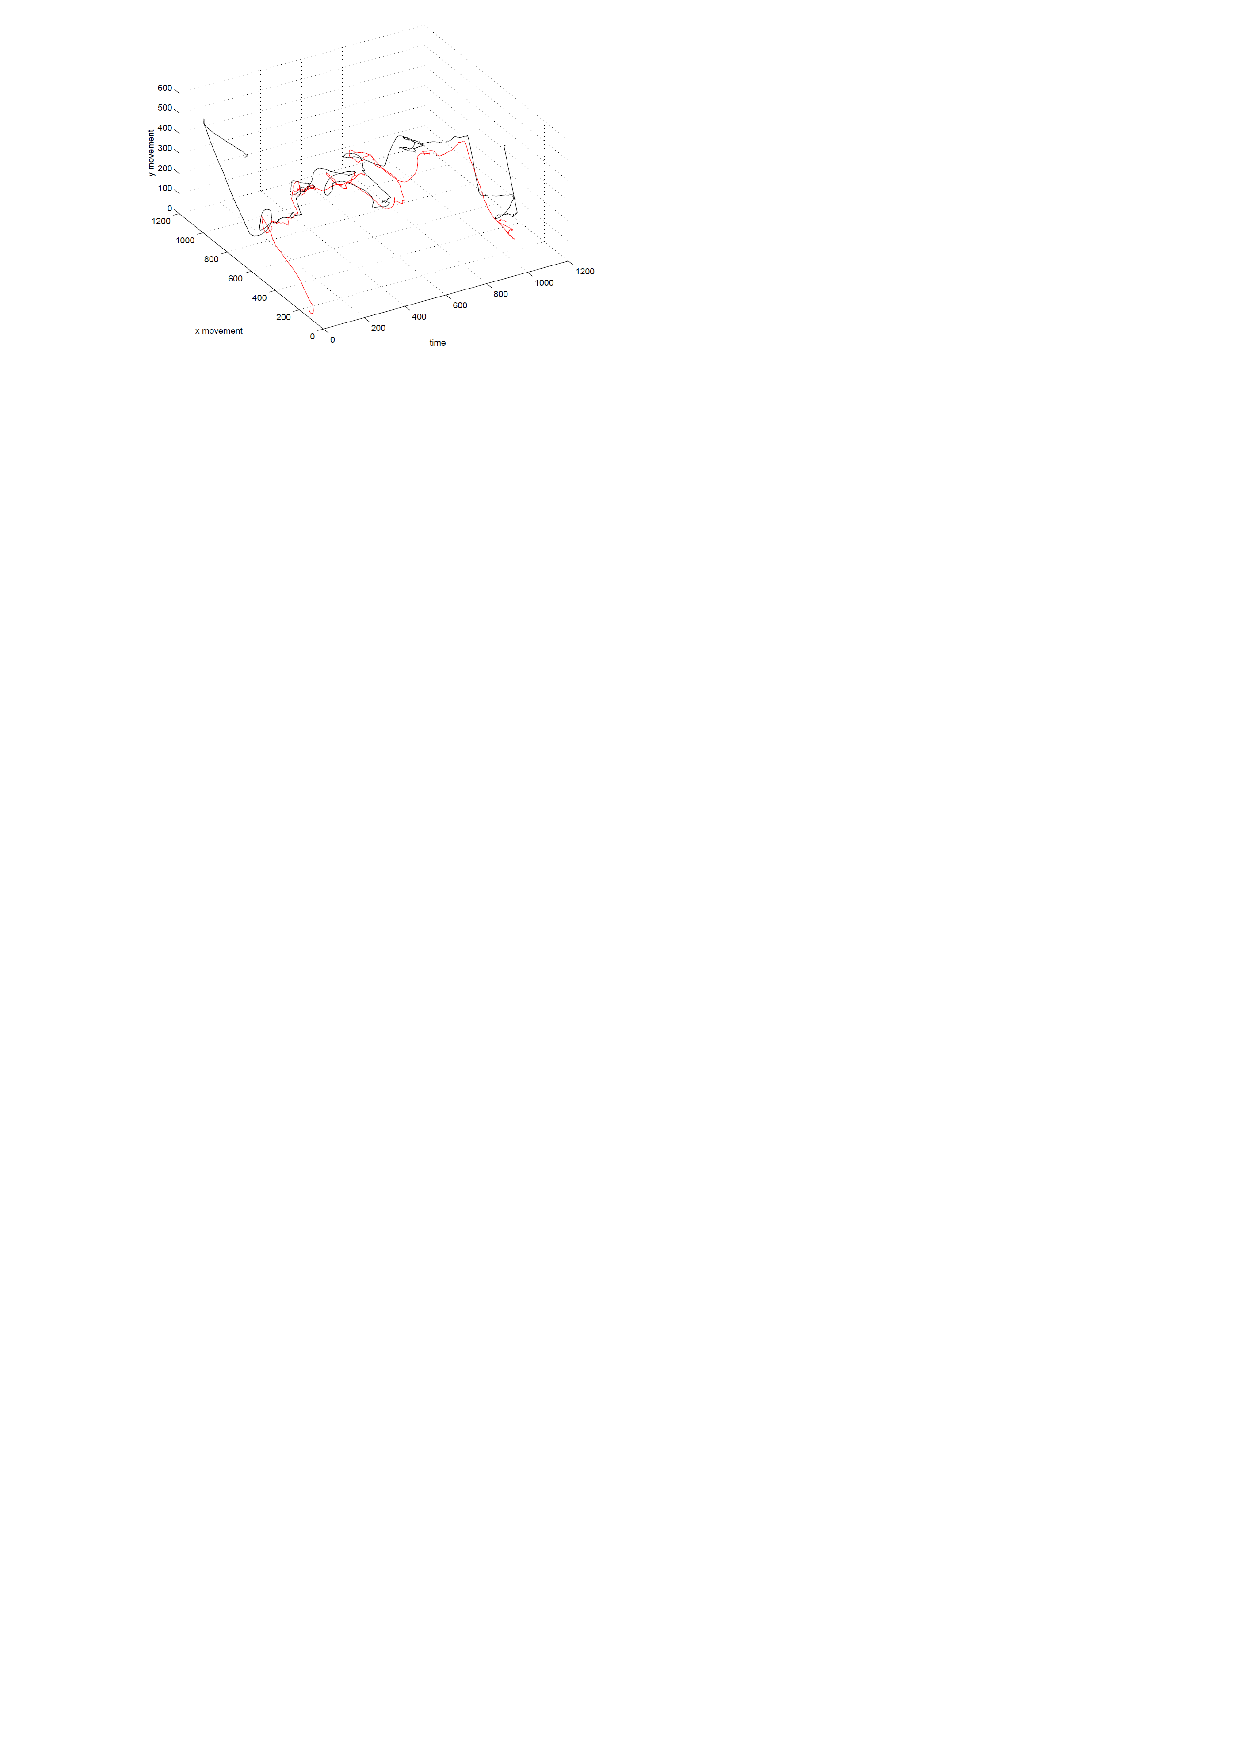
\includegraphics[scale=1]{Gambar/2d_trj}
\caption[Example of 2D trajectories with time component, from \cite{Vlachos:2002}]{Example of 2D trajectories with time component, from \cite{Vlachos:2002}} 
\label{fig:2d_trj}
\end{figure}

The trajectory of a moving object is typically modeled as a sequence of consecutive locations in a multi-dimensional (generally two or three dimensional) Euclidean space \cite{Vlachos:2002}.
Figure~\ref{fig:2d_trj} shows an example of two trajectories from two objects which are moving in a 2D plane.
With their temporal component, we can see that these trajectories are represented as polylines in a 3D space.
 
Nowadays, with the rapid development of technologies in mobile computing and wireless communication, many devices with location acquisition capabilities make it possible to obtain huge volumes of trajectory data from various moving objects.
Furthermore, analysis of trajectory data is an important task for many applications that contain processing and managing moving objects, such as animal movements \cite{Calenge:2009,Nams:2004,Herb:2010,Brillinger:2001}, traffic and transport analysis \cite{Yunyao:1998}, defense and surveillance areas \cite{Ng:2001}, oceanographic observations\footnote{W.S. Kessler, ``Argo work in the coral sea.''http://faculty.washington.edu/kessler/noumea/gliders/\\argo\_coral\_sea.html, March 2010.}, weather and natural phenomena \cite{Hubert:1957}, people behavior \cite{Fuentes:2001} and sports \cite{Brillinger:2007,Iwase:2002}.

Previous work on trajectory data analysis shows that there are several ways to analyze sets of trajectories.
For example, similarity between trajectories can be determined \cite{VlachosGunopoulos:2002,Lin:2005,Kreveld:2007}.
Trajectories can also be clustered into groups with similar characteristics \cite{Gaffney:1999,Lee:2007,Nanni:2006,Buchin:2009}.
Other examples are common data mining tasks such as classification \cite{Lee:2008,Garcia:2006} and outlier detection \cite{LeeHan:2008}.
Furthermore, interesting movement patterns such as flocking can also be computed from a set of trajectories \cite{Gudmundsson:2006,Buchin:2008,Gudmundsson:2007,Laube:2006}.

Even though analysis and research on trajectories has expanded in recent years, several basic concepts still need to be studied further.
Some of them are the median and the mean trajectory for a collection/set of trajectories.
The median and the mean trajectory share some common properties: they should be similar to other trajectories in the set and all parts of them should be located roughly in the middle of the set.
However, there are several important differences between them:
Firstly, the median trajectory must use only parts of trajectories in the set. 
It uses only parts of one trajectory or combines parts from many different trajectories.
This property might be a disadvantage for the median because some parts of it can be located not in the middle of the set, but in several situations this might be useful.

Figure~\ref{fig:mean_dis} shows a set of four trajectories which avoid the light-blue obstacle.
The possible mean trajectory (the black trajectory in the right-hand side of the figure) will pass through the obstacle because the mean must lie in the middle of all trajectories in the set.
In this case, it is clear that the mean trajectory is not suitable for a path of a moving object.

The median trajectory (black trajectory in the left-hand side of the figure) gives a more suitable path because it always uses parts of other trajectories.
In parts near the obstacle, the median is not really in the middle of other trajectories.

\begin{figure}
\centering

\includegraphics[scale=1]{Gambar/mean_dis}
\caption[Example of the median (left) and the mean (right) trajectory \cite{Lionov:2009}]{Example of the median (left) and the mean (right) trajectory \cite{Lionov:2009}} 
\label{fig:mean_dis}
\end{figure}

Secondly, the median trajectory is more robust against outliers than the mean trajectory.
Figure~\ref{fig:robust_med} shows this situation: we add one trajectory (with purple color) which can be categorized as an outlier compared to other trajectories. 
While the median trajectory only needs to be modified a little bit, the mean trajectory has to be changed a lot (comparing to the mean trajectory in Figure~\ref{fig:mean_dis}), to keep it in the middle of other trajectories.

\begin{figure}
\centering
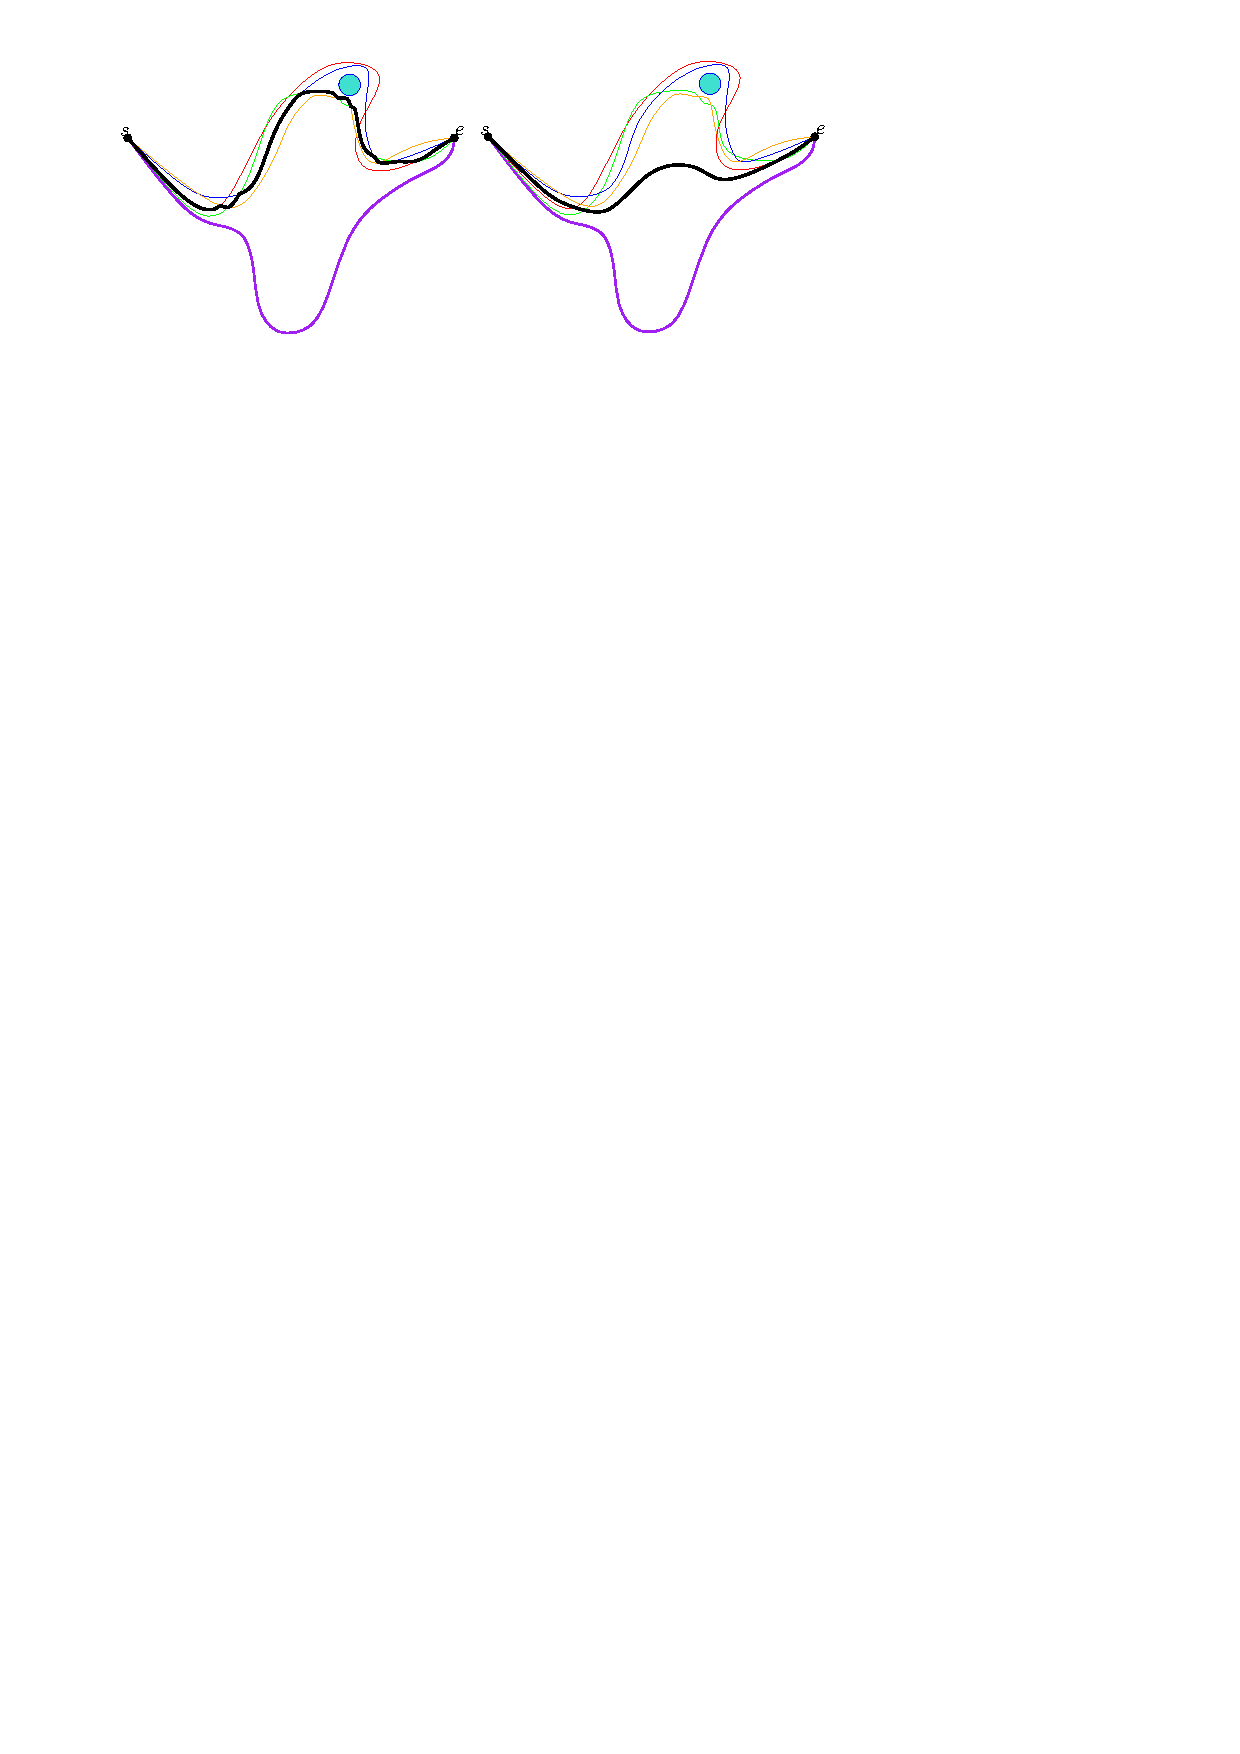
\includegraphics[scale=1]{Gambar/robust_med}
\caption[Robustness of the median trajectory]{Robustness of the median trajectory} 
\label{fig:robust_med}
\end{figure}

In this thesis, we will not cover the mean trajectory and only discuss the median trajectory and algorithms to compute it.
We also ignore the temporal component of the trajectory because it is not clear yet how to take it into account when computing the median trajectory. 
However, some research on motion and kinetic data structures contains a temporal component and are related to the median/mean trajectory \cite{Agarwal:2003,Agarwal:1997}. 

For other types of data, a median has a clear definition.
The median from a population (or a sample) of integer numbers is the number that separates the population into two halves, where at most half of the population have a smaller value and the other half of the population have a larger value than the median. 

For geometric data types, the concept of median also exist.
A \textit{center point} of a set $P$ of $n$ points in the plane is a point such that any closed half-plane whose bounding line contains the center point, contains at least $n/3$ points of $P$ \cite{Amenta:2000}.
If we force the center point to be one of the points from $P$, then we obtain a 2-dimensional version of the median, although the ``quality'' of this median can be bad.

The median trajectory does not have any formal definition yet.
Based on several properties that we mention earlier, such as its similarity with other trajectories and lying approximately in the middle of the set, we can determine a possible median, which can useful in several ways:

\subsection{Determine the most typical trajectory}
The property of the median trajectory makes it suitable to analyze the movement behavior or movement pattern from a group of same objects because the median somehow represents the whole trajectories in the set/collection.
The median trajectory properties, such as the length, the direction or the average speed (if we include the temporal component), could give valuable information.

Example applications include the detection of outliers, which can be done by analyzing the length and the similarity of the shape of the median with other trajectories.
Analyzing the average speed together with the shape of the median trajectory might be useful to understand the behavior and the movement pattern of people walking around in an area which has several interesting places to be visited (e.g., a zoo or an amusement park). 

\subsection{Better visualization for a set of trajectories}
Visualization of the median trajectory, together with its set of trajectories, might give the viewer a better interpretation and information about the set of trajectories.

\begin{figure}
\centering
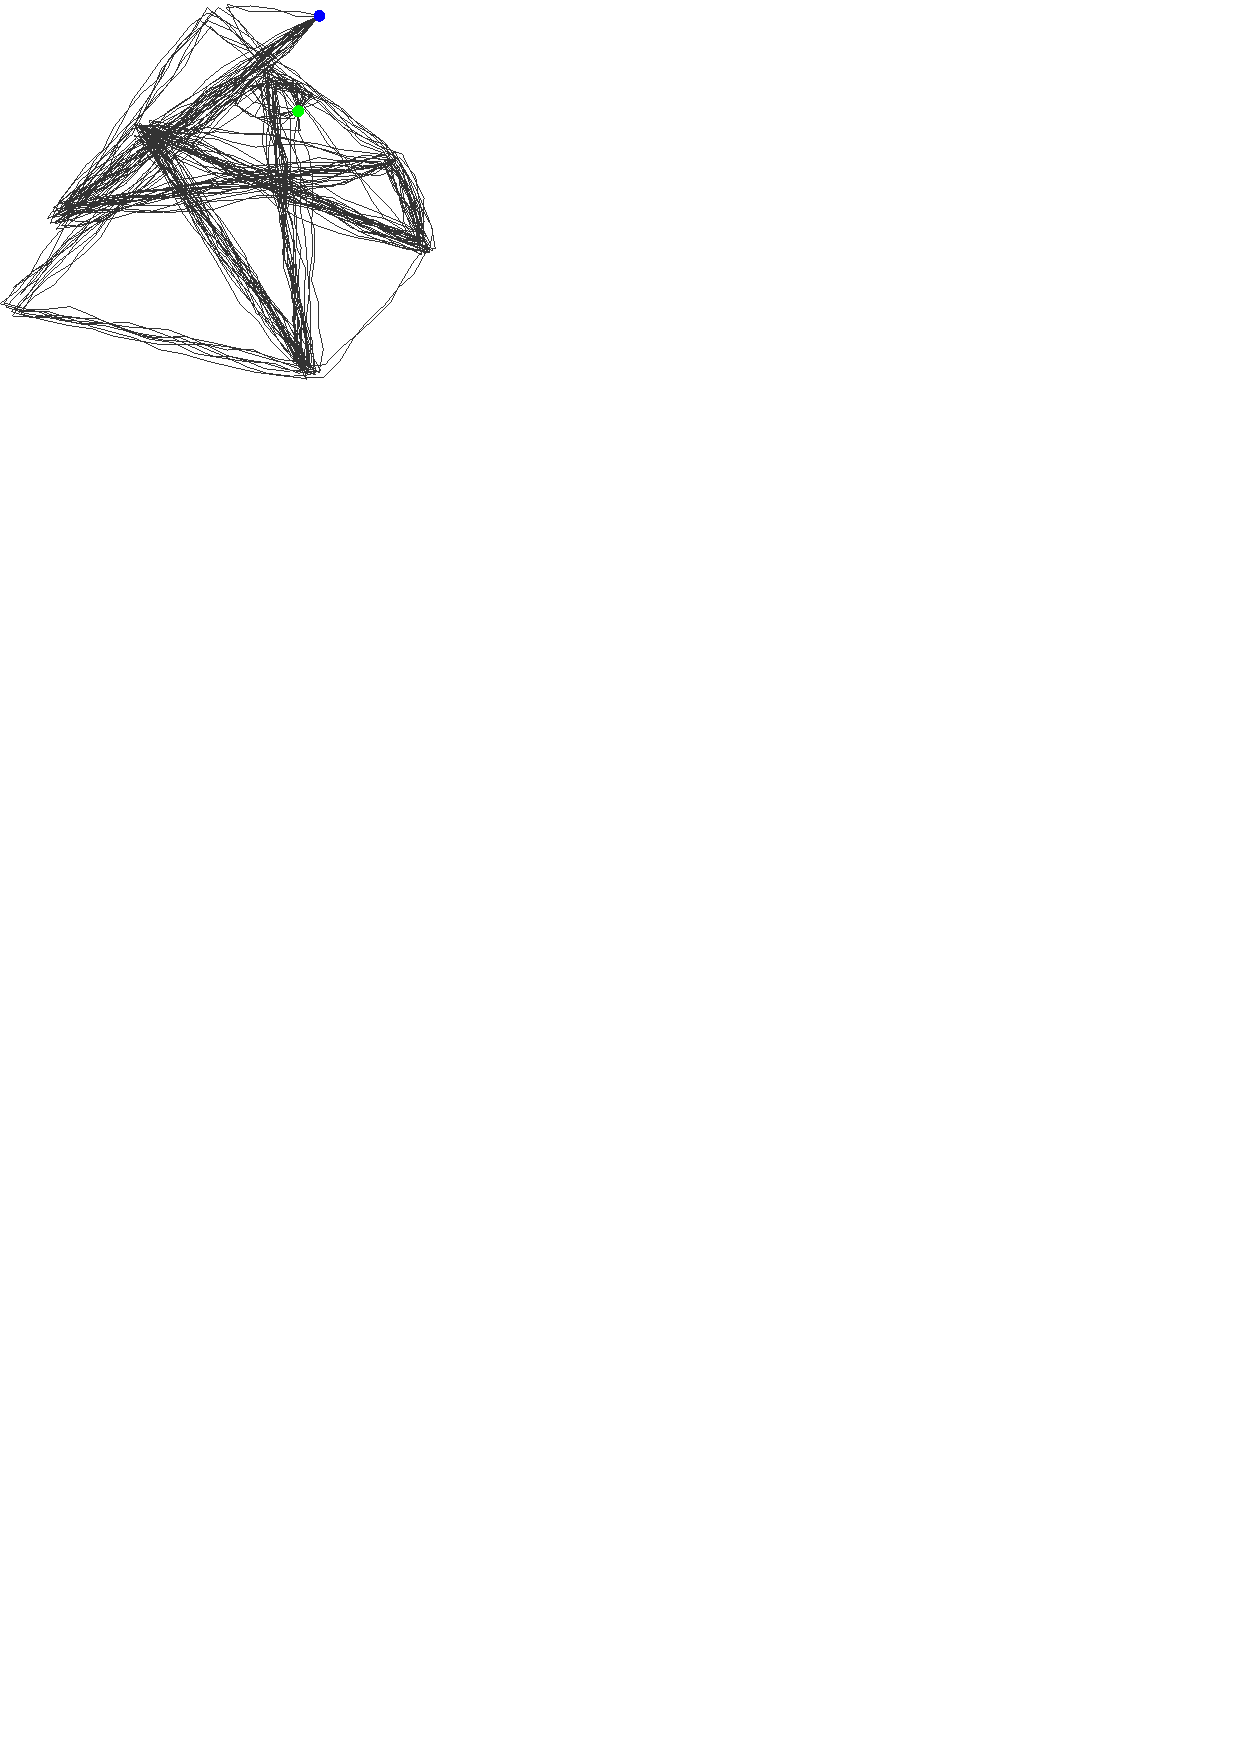
\includegraphics[scale=1]{Gambar/all30_visual}
\caption[The set of 30 trajectories, starting at the blue point \& ending at the green point]{The set of 30 trajectories,starting at the blue point \& ending at the green point} 
\label{fig:all30_visual}
\end{figure}

\begin{figure}
\centering
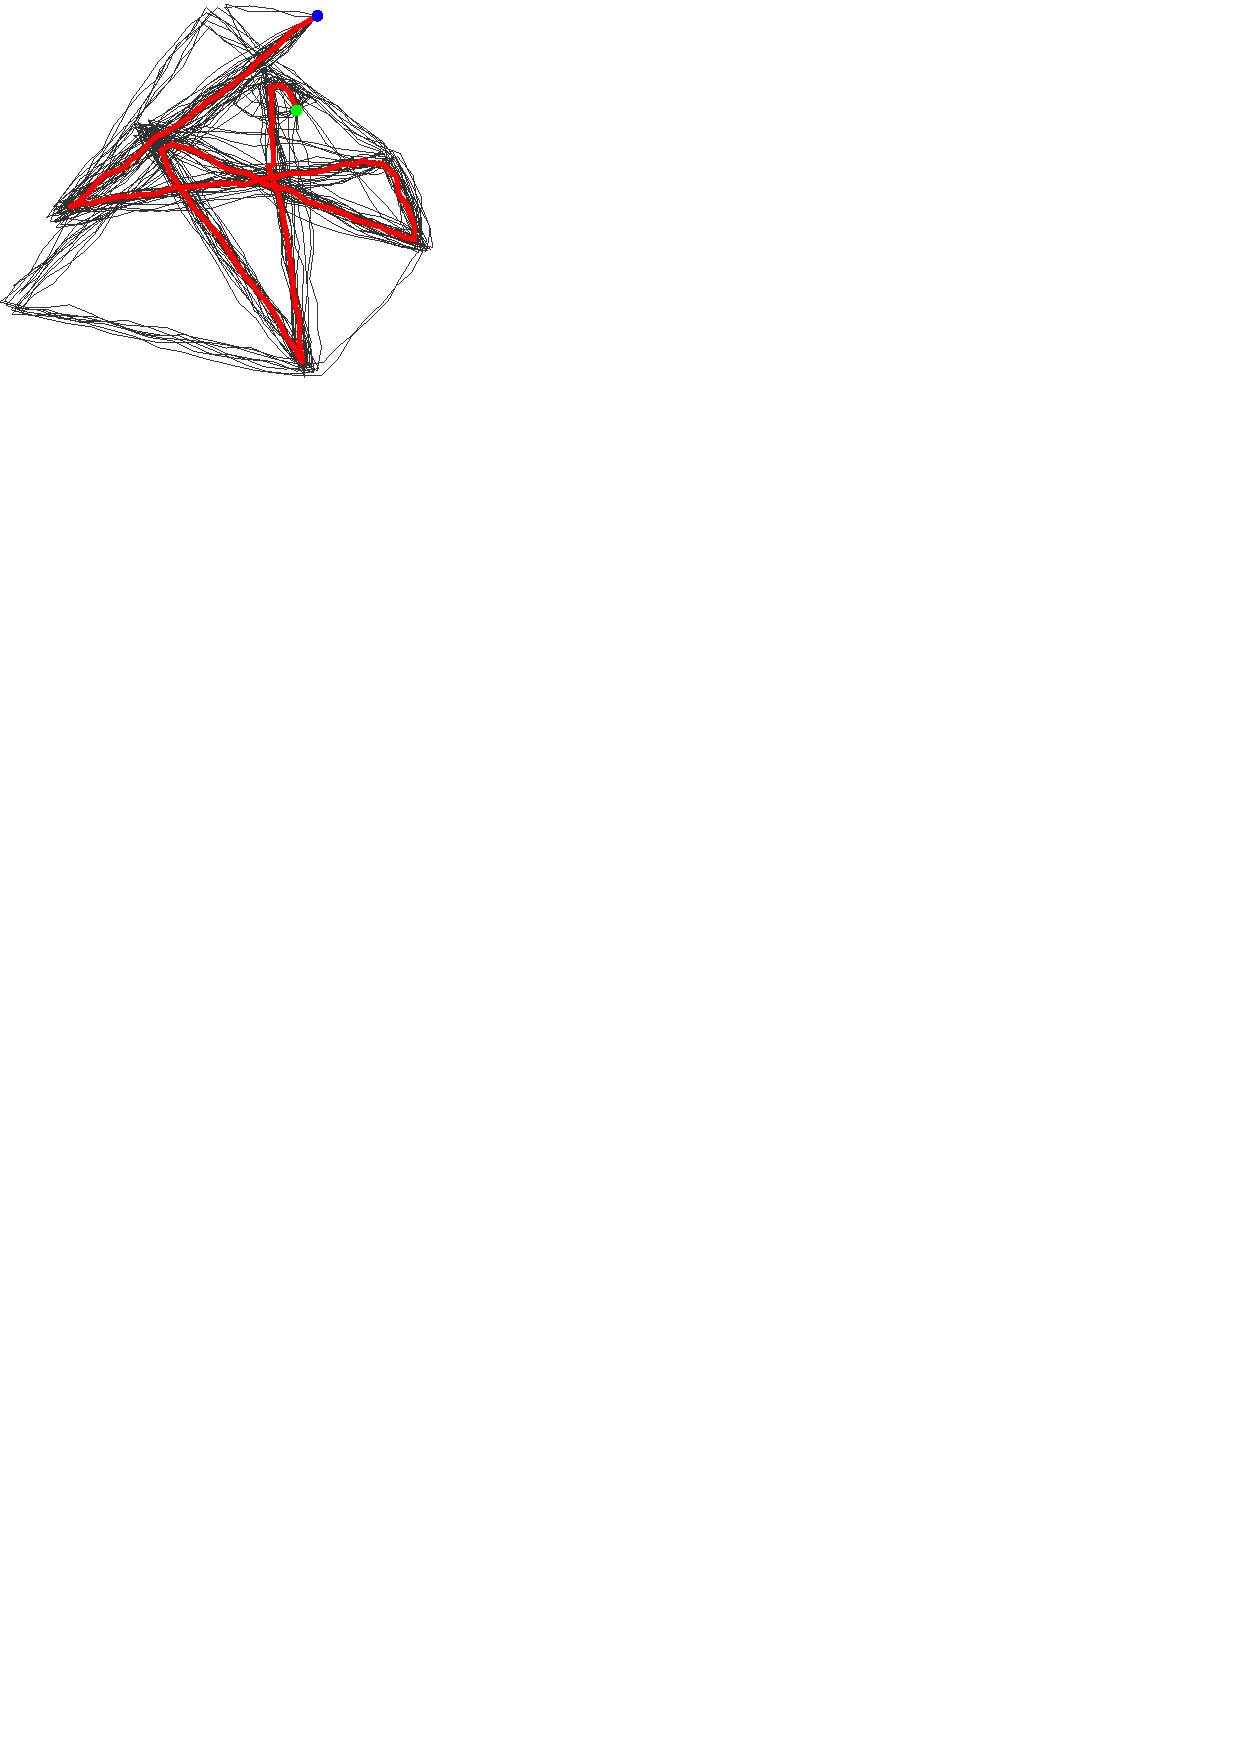
\includegraphics[scale=1]{Gambar/med_visual}
\caption[A set of 30 trajectories with its possible median trajectory]{A set of 30 trajectories with its possible median trajectory} 
\label{fig:med_visual}
\end{figure}

We give an example in Figure~\ref{fig:all30_visual}, where a set has 30 trajectories, which is paths of 30 objects moving from the blue point to the green point.
From this figure, we can hardly tell anything about the general behavior or the direction of these trajectories. 
However, we know that several trajectories are different than others and probably can predict what the majority does, but it is still difficult to visualize what the majority of these trajectories does.

In the following figure (Figure~\ref{fig:med_visual}), we present a possible median trajectory as the red and thick trajectory.
From this visualization, it is clear what the majority of trajectories does.
Moreover, we can identify what parts of some trajectories are completely different from others. 

The visualization of the median trajectory could be useful in some real-life applications:
The median trajectory from trajectories of visitors in a national park can be used to see the most common path taken by visitors, which is probably the path that is preferred by future visitors.
This information might be useful if we want to create a map that can help those visitors by providing valuable information about a path and direction on that national park in the map, so that he/she can decide which path that he/she will take. 
% Other example is to use the median trajectory for video surveillance. 
% where median trajectory shows the most common path that the visitor take, and identify if there are any unusual trajectory

\subsection{\texorpdfstring{$k$}{k}-medoid clustering}
Another application that could use the median trajectory is the $k$-medoid algorithm, which is used in cluster analysis.
The $k$-medoid clustering algorithm is related to the $k$-means algorithm, a method to partition/group a set of objects into $k$ different clusters containing similar objects.

In general, each cluster in both algorithms has one object act as a \textit{central object} and other members of the cluster should be similar or having a small distance to this object.
The similarity or the distance between objects can be measured using different distance functions (e.g. Euclidean distance, Minkowski distance, etc), depending on the type of objects and the purpose of the clustering.

The main difference between the two algorithms is on the selection of the central object for each cluster. 
While the $k$-means simply uses the mean of objects, the $k$-medoid must use the medoid (an object which has the smallest average of dissimilarity/distance to all other objects in the set, but it must be a member of the set). 
This implies that $k$-means could create a new object to be the central object whereas the $k$-medoid must use one of the objects from the set.
Thus, the $k$-medoid algorithm is more suitable for spatial clustering purposes and less sensitive against noise and outliers.  

Partitioning Around Medoids (PAM) ~\cite{Kaufman:2005} is a basic $k$-medoid clustering algorithm.
It works as follow:
\begin{enumerate}
\item
Define a value $k$ and choose $k$ objects as a set of medoids.
\item
Assign every object to its closest/similar medoid and after that, compute the cost for the whole configuration.  
\item
Find another configuration by selecting a pair of medoid and non-medoid objects which have the smallest distance cost and swapping them temporarily.
Then, we assign all other objects to this temporary set of medoids and obtain a new configuration.
\item
If the new configuration has smaller cost than the last configuration, then we change the set of medoids and return to step 3
\item
Otherwise, stop and we find the set of medoids with their non-overlapping set of clusters.
\end{enumerate}

In case we want to cluster a set of trajectories, we can use the median trajectory as a medoid in this algorithm.
However, some changes probably should be made.
For example, finding another configuration is not done by simply swapping the median with other trajectory, instead we can choose to swap part of them (with the requirement that both trajectories intersect one another).

\section{Basic Idea of the Research}
\label{sec:basic_idea}

Consider a set $T$ of $m$ trajectories.
We want to to compute the median trajectory of $T$.
In this set, all trajectories have the same start and end points.
The median trajectory of $T$ must be built using parts of trajectories in $T$ and somehow must follow what other trajectories in $T$ do, while staying in the ``middle'' of other trajectories.

\subsection{The Simple Switching Method }
\label{sec:switch}

A simple idea to obtain a median trajectory from $T$ is to start from the ``middle'' trajectory, which is the $(m+1)/2$-level of arrangement formed by all trajectories in $T$ (we assume $m$ is odd).
At every intersection point, the median trajectory will switch to another trajectory and keep $(m+1)/2$ trajectories above and below the median \cite{Buchin:2010}.

\begin{figure}
\centering
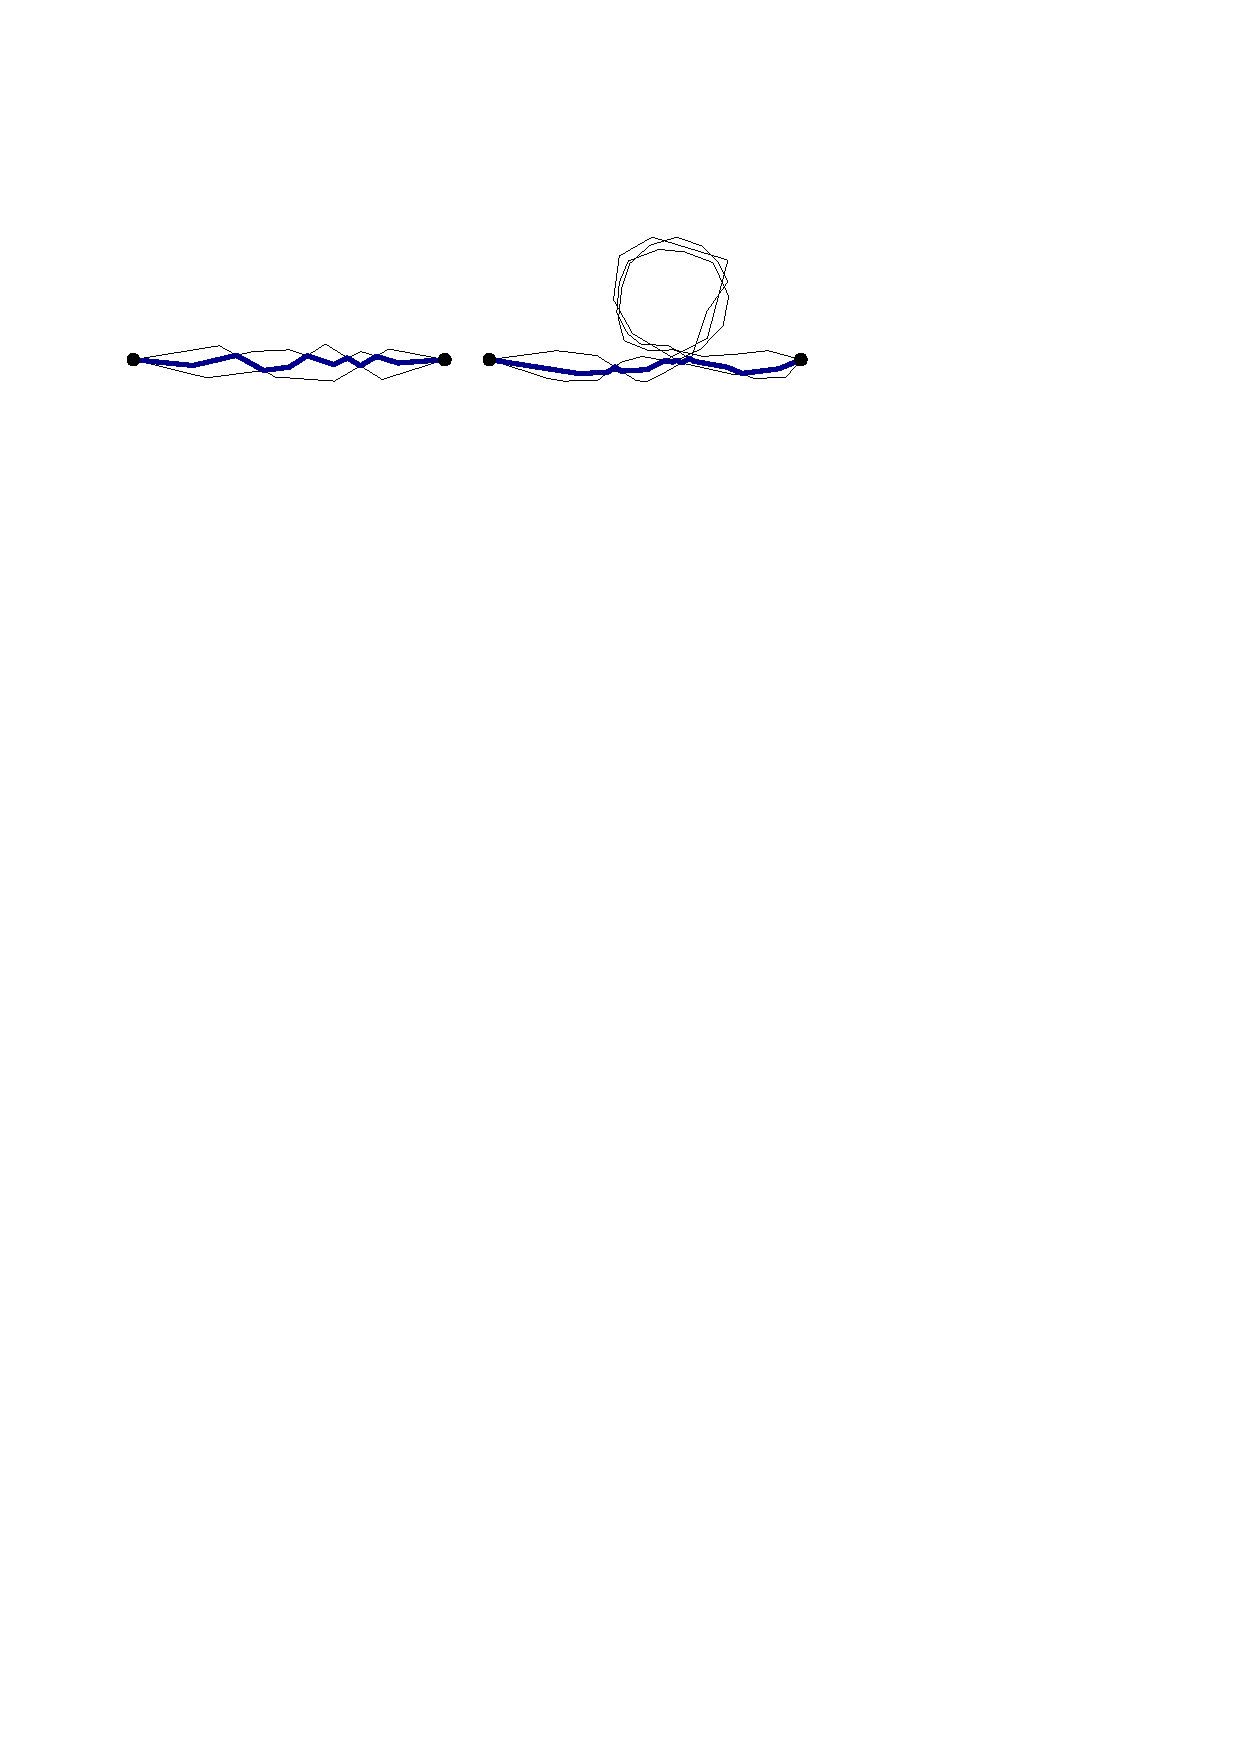
\includegraphics[scale=1]{Gambar/switch_fail0}
\caption[Illustration of the simple idea using switching]{Illustration of the simple idea using switching} 
\label{fig:switch_fail0}
\end{figure}

\begin{figure}
\centering
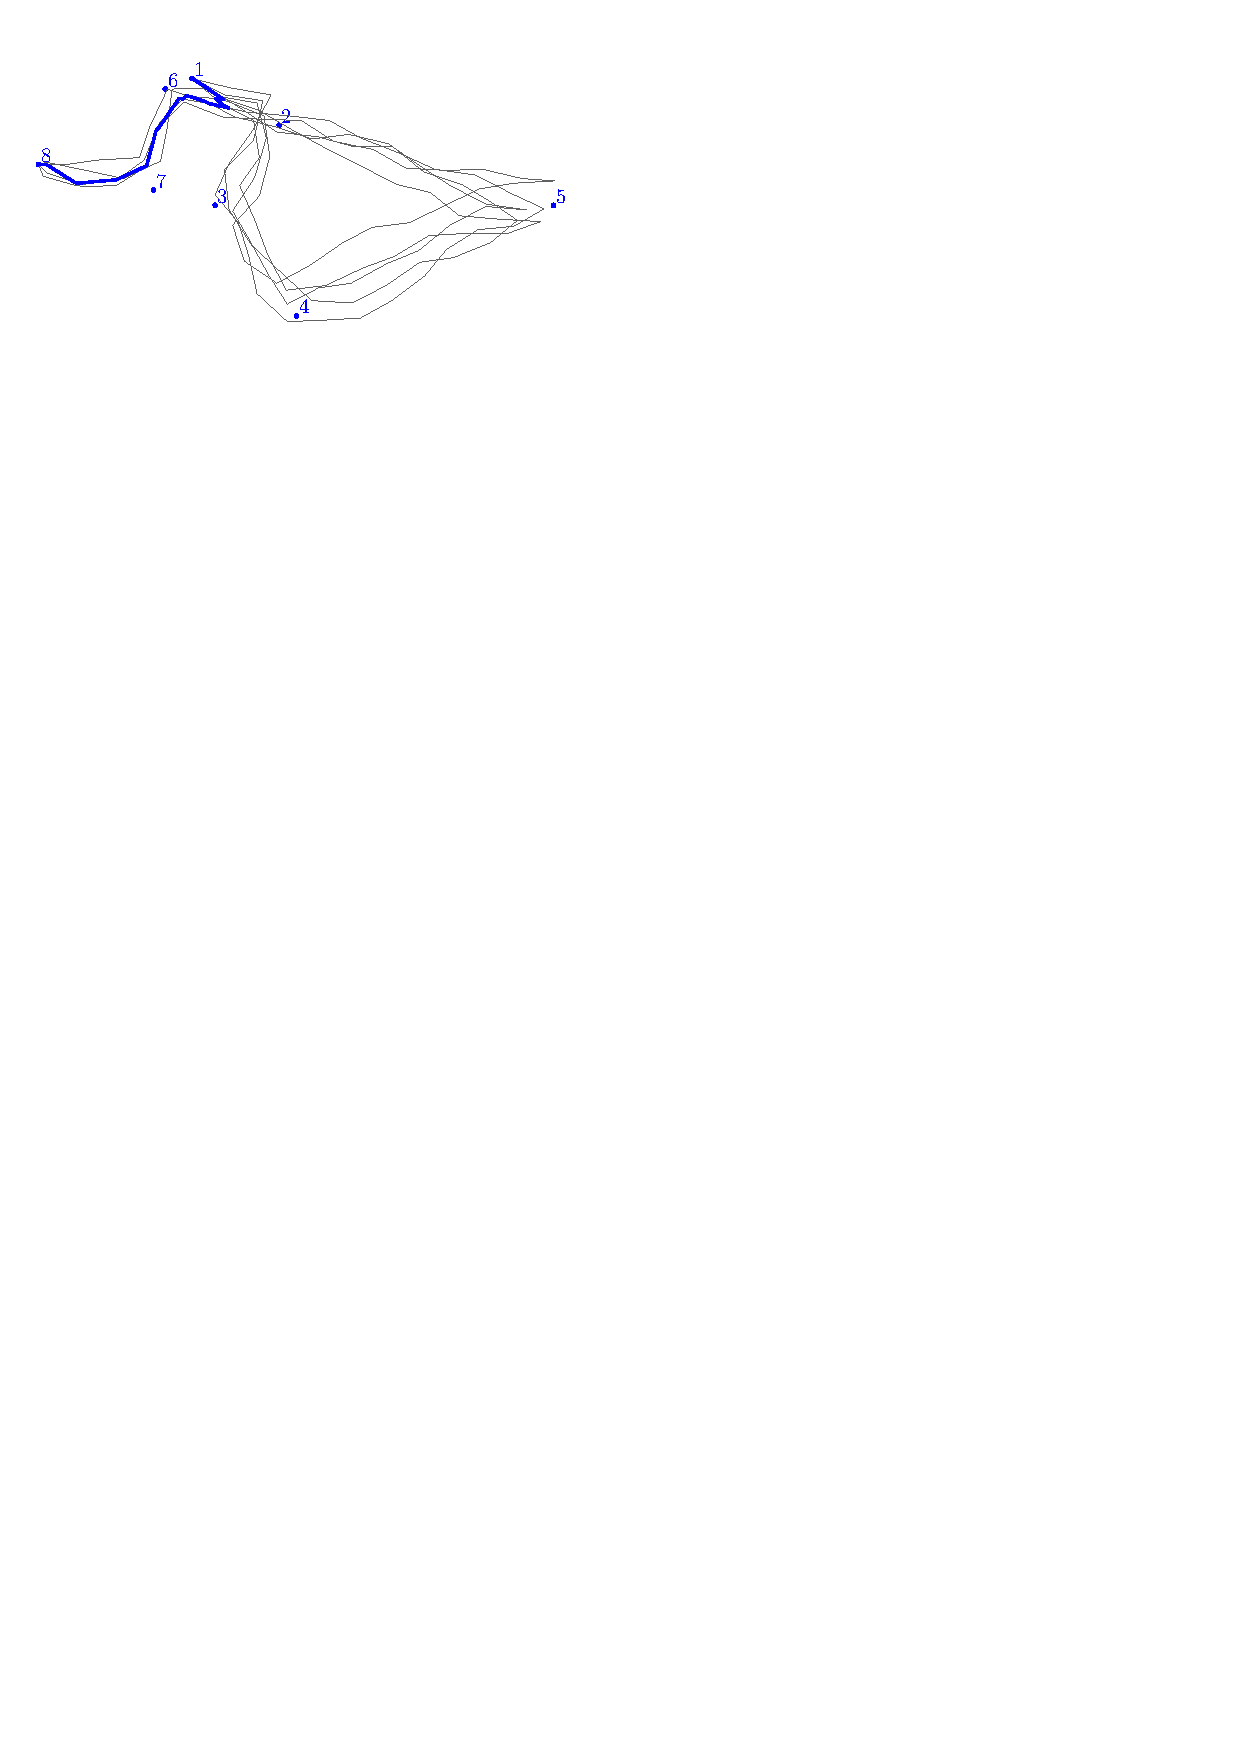
\includegraphics[scale=1]{Gambar/switch_fail1}
\caption[The median trajectory make a shortcut path \cite{Lionov:2009}]{The median trajectory makes a shortcut \cite{Lionov:2009}} 
\label{fig:switch_fail1}
\end{figure} 

Figure~\ref{fig:switch_fail0} shows the result (the median trajectory is the thick-blue trajectory) of this approach for two different types of set of trajectories, one of them contains trajectories with self intersection.
From the right-hand side of the figure in Figure~\ref{fig:switch_fail0}, we can see that this method cannot produce suitable median trajectory because the median does not follow the loop created by the three trajectories.

In general, this method will not give a suitable median if a set of trajectories contains self-intersecting trajectories.
More examples from \cite{Lionov:2009} show several ``incorrect'' median trajectories obtained by using this simple switching method.
The blue median trajectory in Figure~\ref{fig:switch_fail1} makes a shortcut path to the end point.

\begin{figure}
\centering
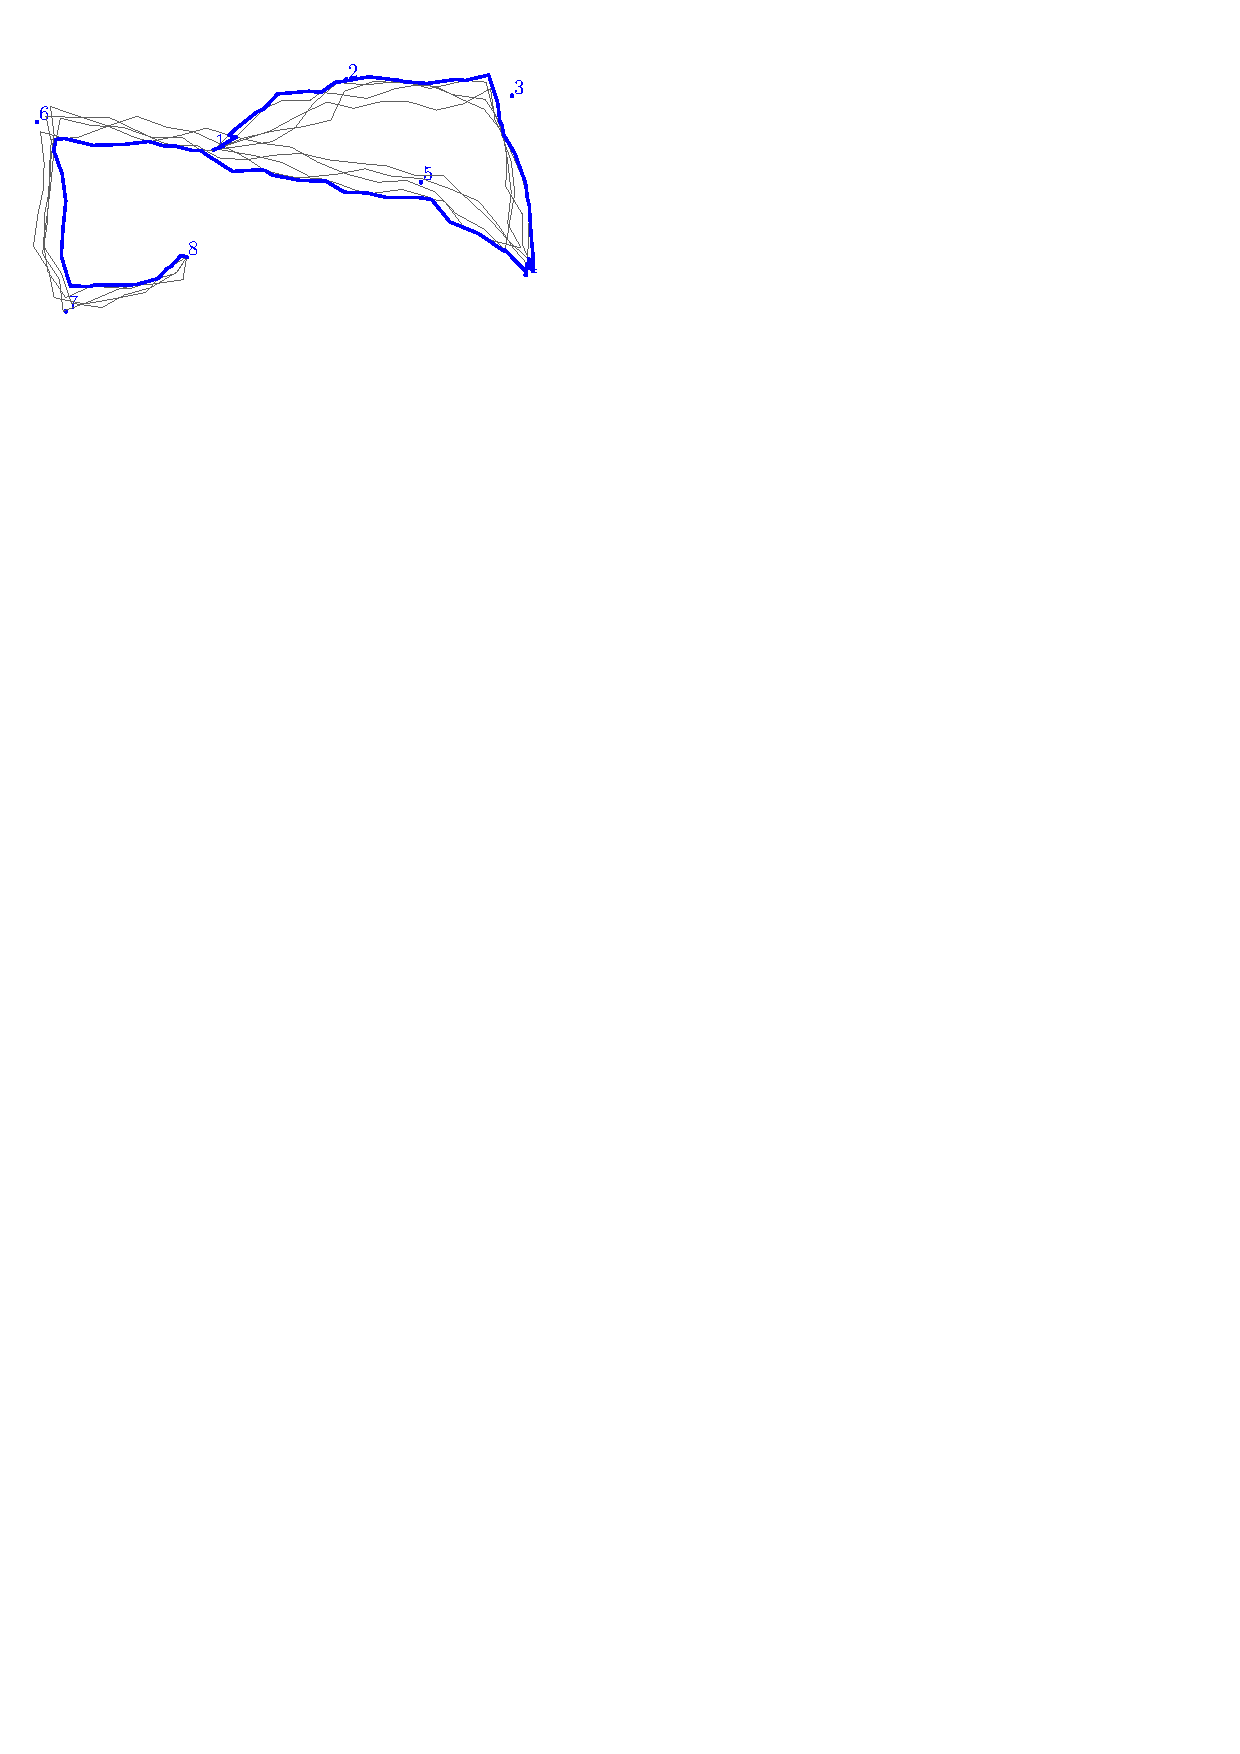
\includegraphics[scale=1]{Gambar/switch_fail2}
\caption[The median trajectory does not stay in the middle \cite{Lionov:2009}]{The median trajectory does not stay in the middle \cite{Lionov:2009}} 
\label{fig:switch_fail2}
\end{figure} 

The median trajectory in Figure~\ref{fig:switch_fail2} does not stay in the "middle" of other trajectories.
Finally, in Figure~\ref{fig:switch_fail3}, the median trajectory does not follow the sequence of regions as the other trajectories. 
The correct sequence of regions is $1-2-3-4-5-6-7-8$.

\begin{figure}
\centering
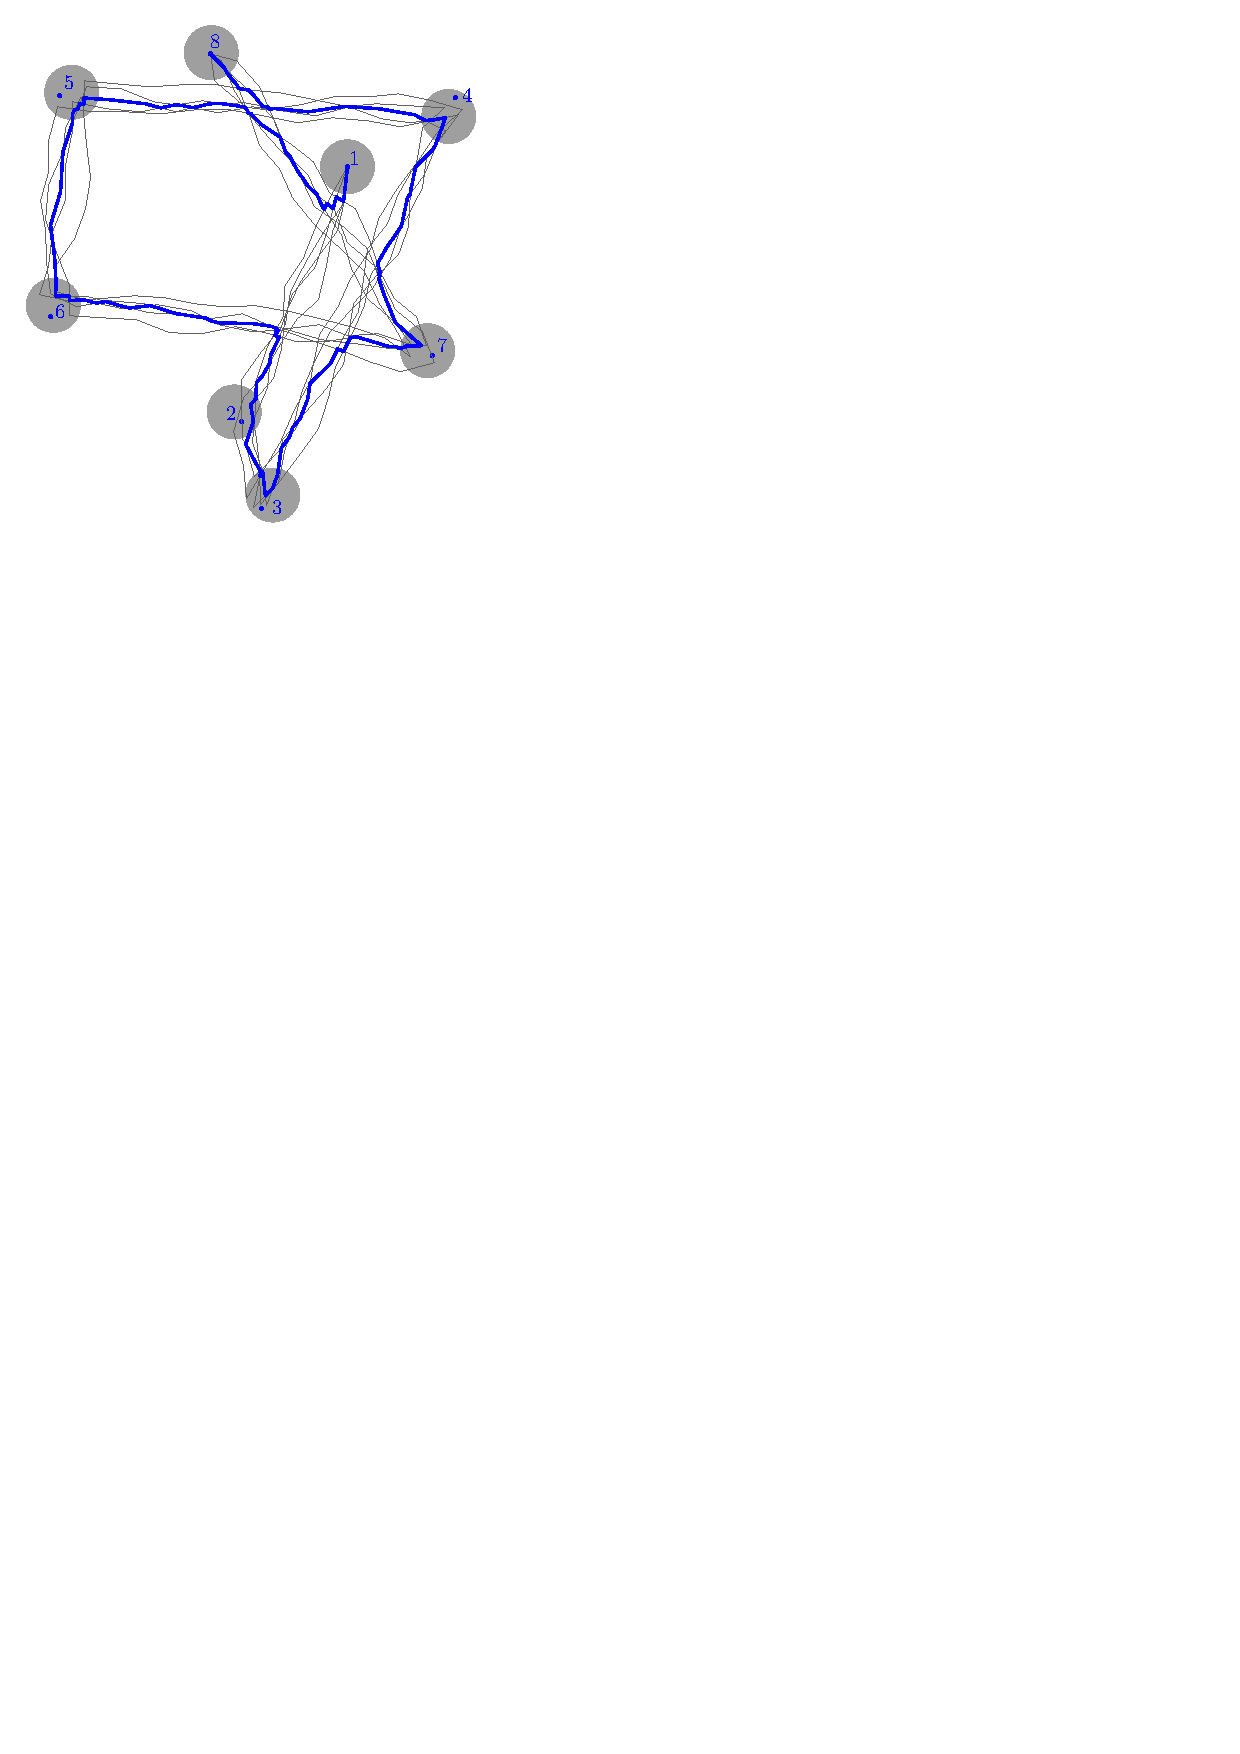
\includegraphics[scale=1]{Gambar/switch_fail3}
\caption[The median trajectory follows incorrect direction \cite{Lionov:2009}]{The median trajectory does not follow the correct sequence of regions \cite{Lionov:2009}} 
\label{fig:switch_fail3}
\end{figure} 
 
\subsection{The Algorithm Using the Concept of Homotopy}
\label{sec:homotopy}

Another algorithm to compute the median trajectory uses the concept of homotopy (along with the modified simple switching method) \cite{Buchin:2010}.
This algorithm works by placing cross in a relatively large face bounded by segments from a set of trajectories.
Figure~\ref{fig:homotopy} shows an example where cross is placed in the relatively large bounded face and two crosses are placed in the outer face.

\begin{figure}
\centering
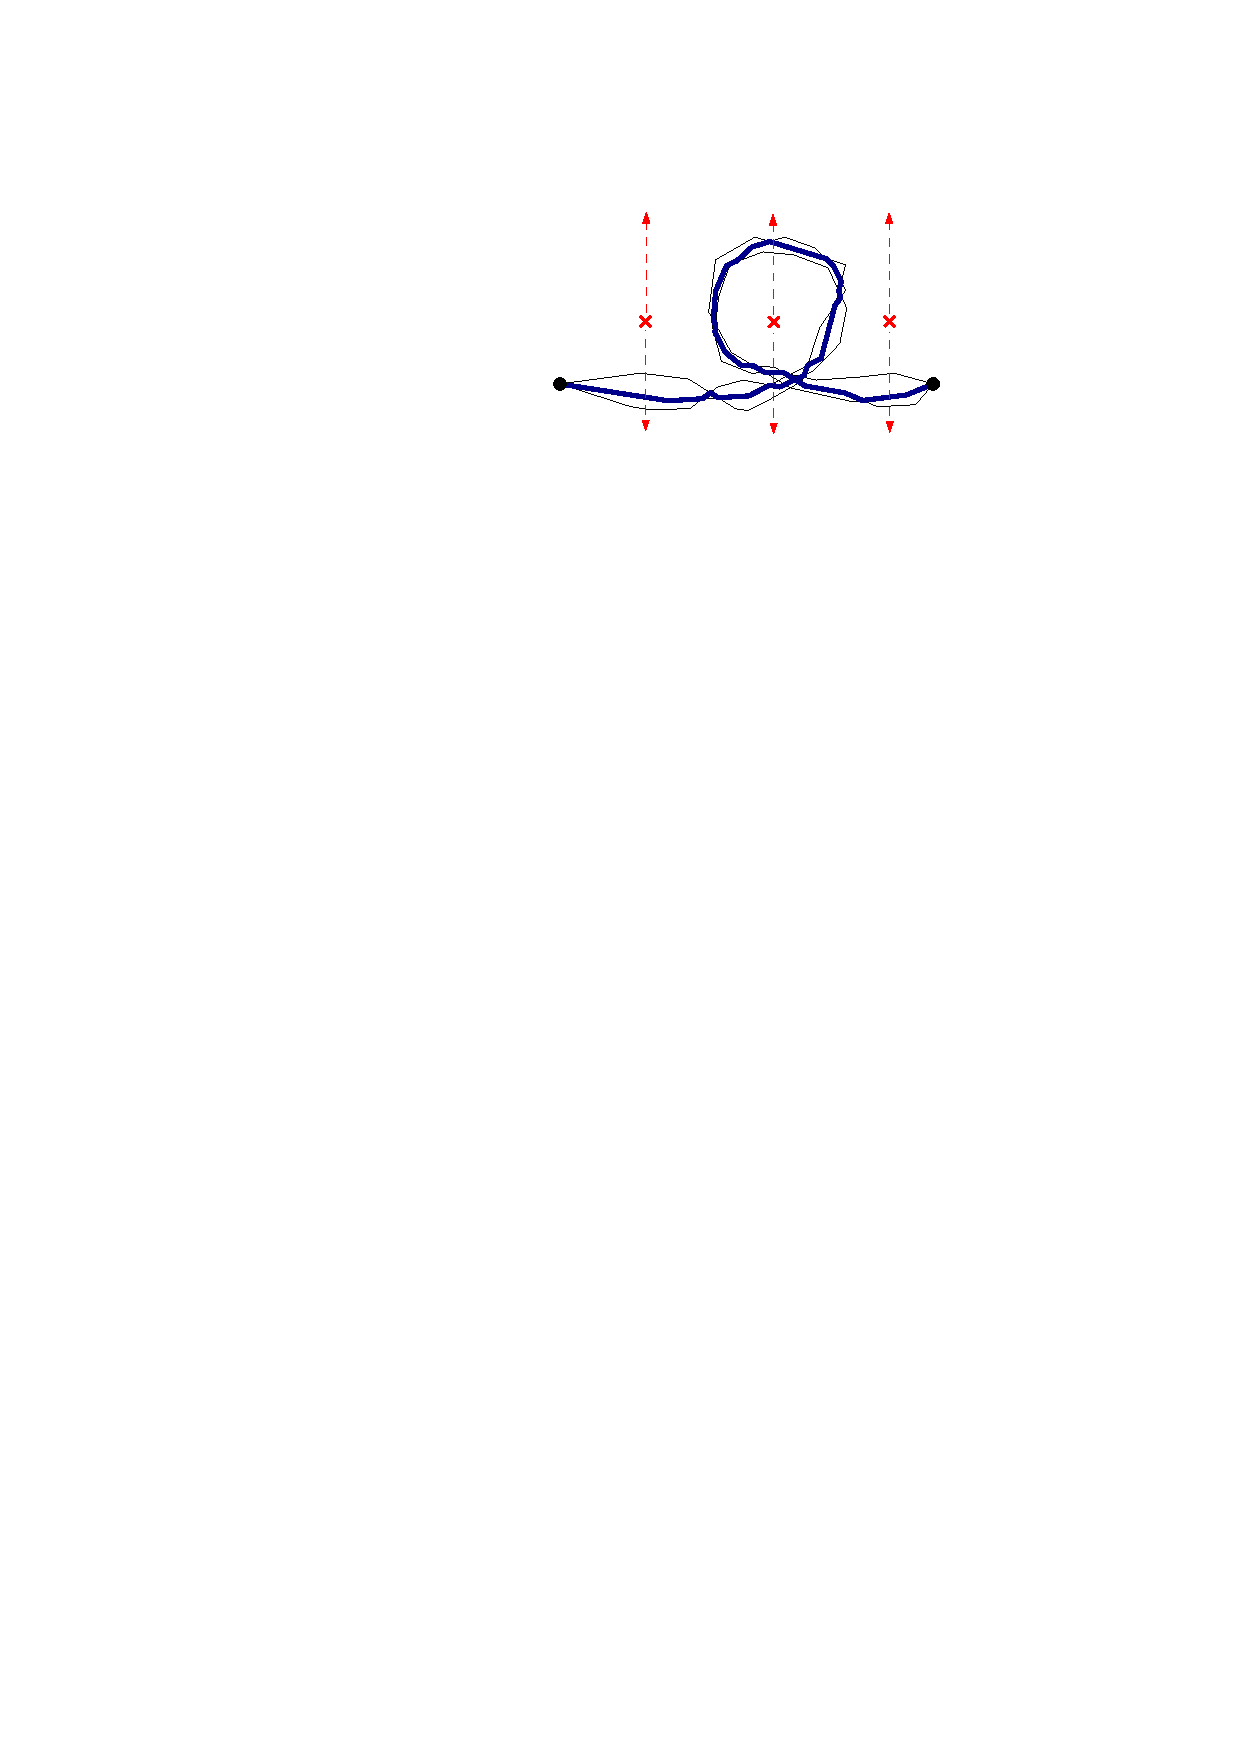
\includegraphics[scale=1]{Gambar/homotopy}
\caption[Illustration of the algorithm using homotopy concept]{Illustration of the algorithm using homotopy concept} 
\label{fig:homotopy}
\end{figure}

Based on the location of these crosses, each trajectory in $T$ will be assigned a \textit{signature}.
Figure~\ref{fig:base_sign} shows three trajectories and two crosses \textit{a} and \textit{b}. 
From these two crosses, four half-lines are created: \textit{$a^{+}$} and \textit{$a^{-}$} are half-lines above and below \textit{a}, while \textit{$b^{+}$} and \textit{$b^{-}$} are half-lines above and below \textit{b}, respectively. 

For all trajectories in $T$, we give them a signature based on how they intersect with the half-line(s) from the crosses. 
Note that each trajectory might have a different signature, because it depends on the position of the trajectory with respect to all crosses in the plane.
In Figure~\ref{fig:base_sign}, the blue trajectory intersect with \textit{$a^{-}$} and \textit{$b^{+}$}, thus its signature will be \textit{$a^{-}b^{+}$} (the order is following the direction of the trajectory). 
In the same way, the signature of the red trajectory will be the same as the green trajectory: \textit{$a^{-}b^{-}$}.

\begin{figure}
\centering
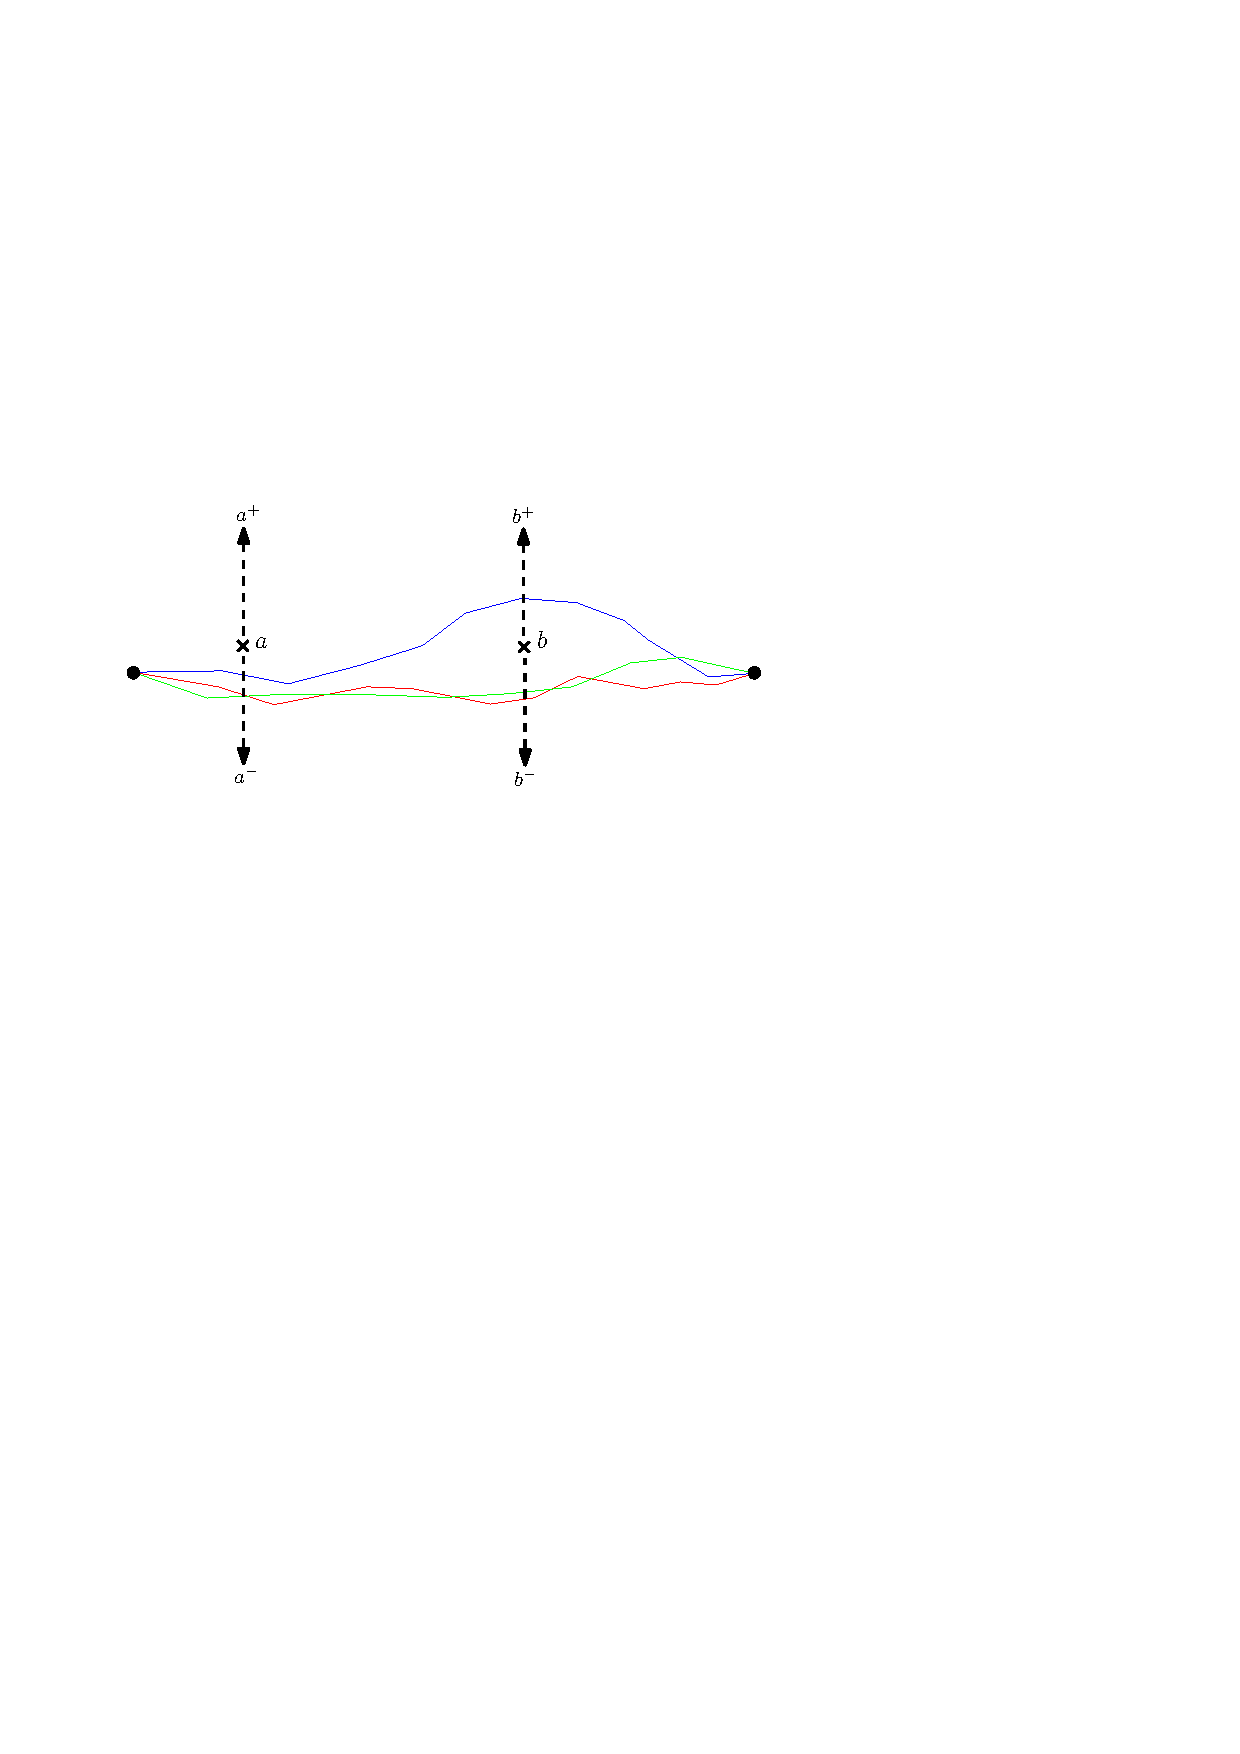
\includegraphics[scale=1]{Gambar/base_sign}
\caption[Trajectories and crosses]{Trajectories and crosses} 
\label{fig:base_sign}
\end{figure}

% The next step of the algorithm is to create the subset $T'$ of $T$.
% All trajectories in $T'$ must be homotopic to each other and also the set with the most number of trajectories from $T$.

Two different trajectories are homotopic if one trajectory can be deformed continuously into the other one without passing through any crosses, while the start and end point are not moved.
Naturally, two trajectories are homotopically equivalent if their signatures are exactly the same. 
However, two homotopic trajectories do not always have the same signatures.
We shown an example in Figure~\ref{fig:diff_sign} where the blue and the black trajectory are homotopic, but their signatures are different.

To determine whether two trajectories with different signature are homotopic or not, we perform a \textit{reduce} operation.
This \textit{reduce} operation works by eliminating two exact same signs, if their position is next to each other in the signature.
In Figure~\ref{fig:diff_sign}, the signature of the blue trajectory is \textit{$a^{-}b^{+}c^{+}c^{+}b^{+}b^{-}c^{-}$}.
Notice that it has two \textit{$c^{+}$} that we can eliminate.
This will change the signature of the blue trajectory into \textit{$a^{-}b^{+}b^{+}b^{-}c^{-}$}.
Once again, we can identify that two \textit{$b^{+}$} are positioned directly to each other. 
Performing the reduce operation again, we will get the final signature of the blue trajectory: \textit{$a^{-}b^{-}c^{-}$}.
At this point, we cannot apply the reduce operation again to this signature, and we say that the signature has been \textit{maximally reduced}.
Finally,we conclude that if two trajectories have the same maximally reduced signature, then the two trajectories are homotopically equivalent.  

\begin{figure}
\centering
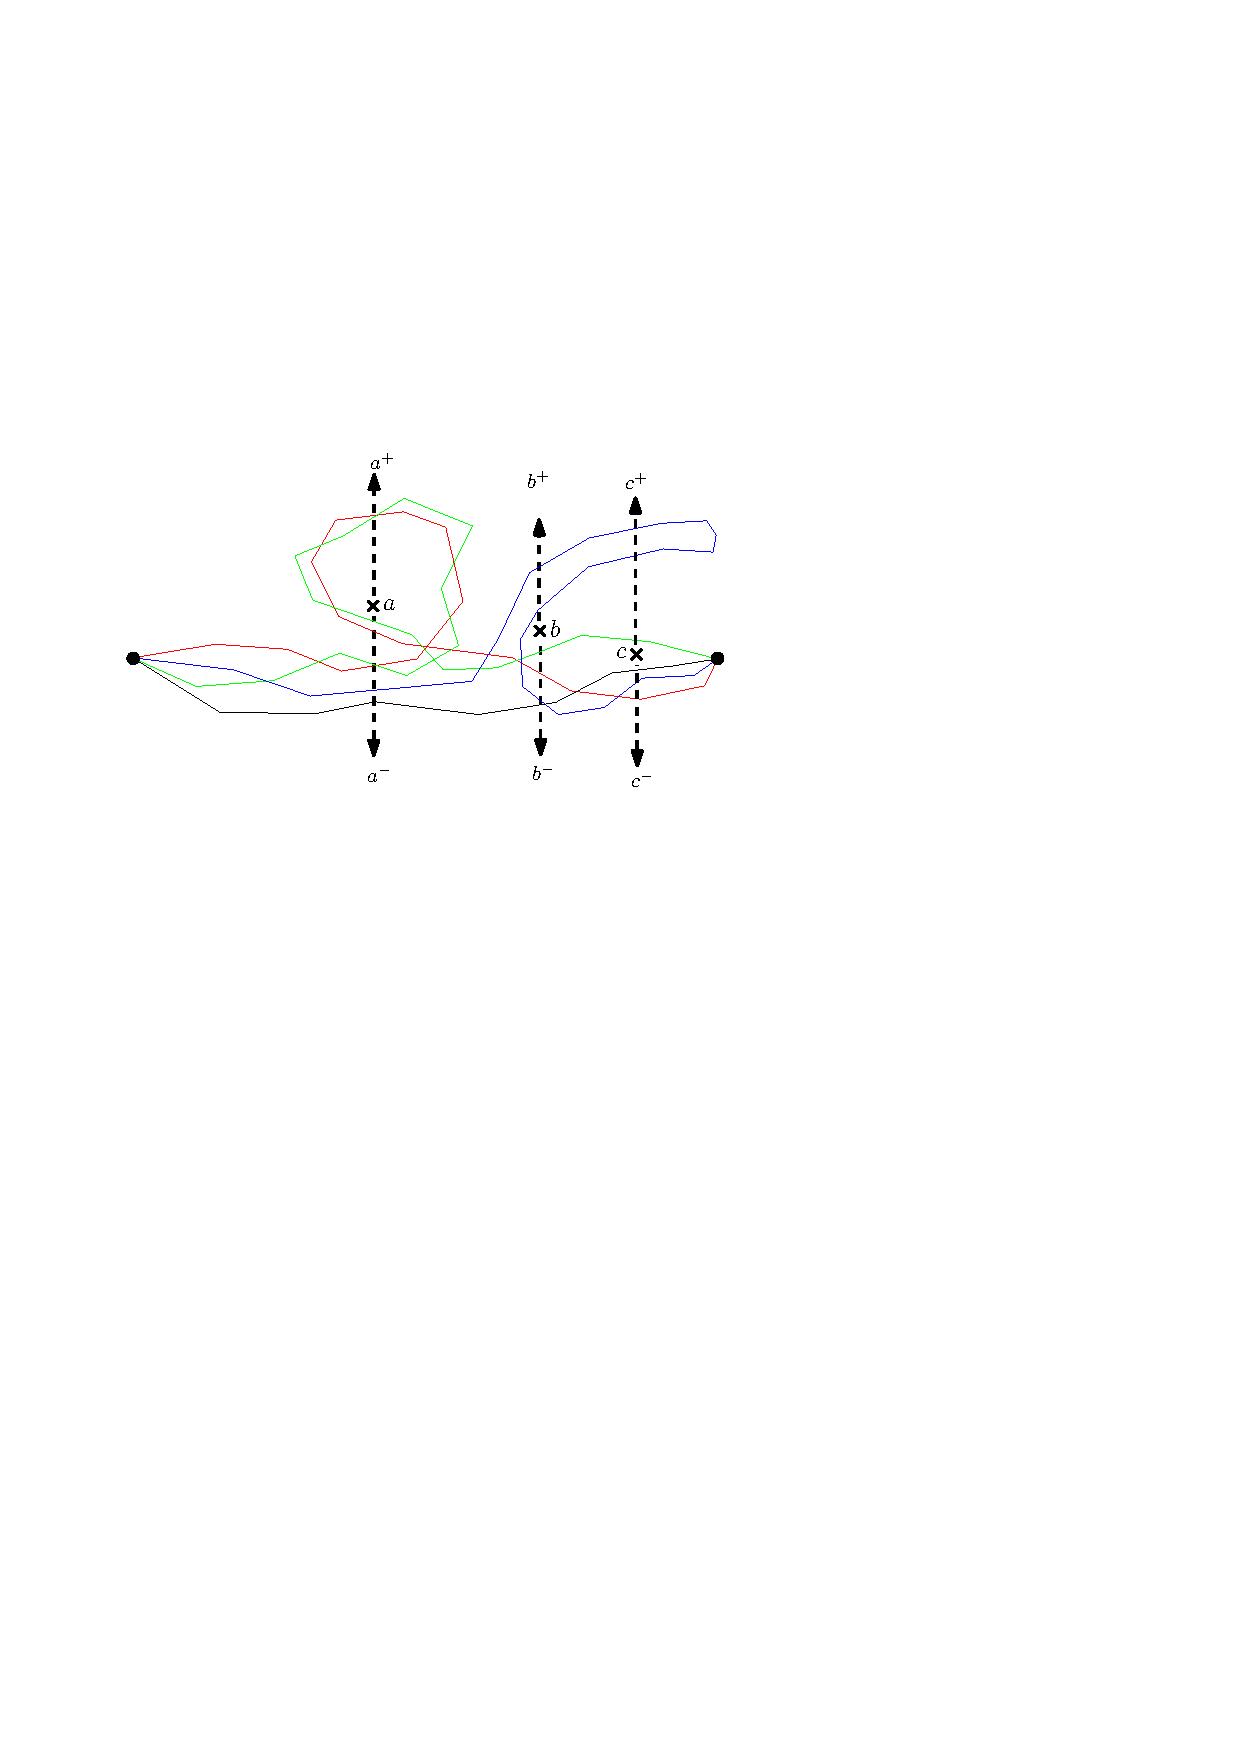
\includegraphics[scale=1]{Gambar/diff_sign}
\caption[The blue and black trajectory are homotopically equivalent \cite{Lionov:2009}]{The blue and black trajectory are homotopically equivalent \cite{Lionov:2009}} 
\label{fig:diff_sign}
\end{figure}

The next step of the algorithm is to create a subset $T'$ of $T$, and then find the median trajectory by using only parts of trajectories from $T'$.
Creating $T'$ is straightforward, we only need to compute maximally reduced signature for all trajectories and choose a subset with the largest number of trajectories which have the same signature.

To create the median trajectory from $T'$, we use the modified version of the switching method.
This method start at the first segment of the``middle'' trajectory.
We find such a segment by determine the outer face of the set of trajectories.
The first segment of the ``middle'' trajectory is the segment where there are $(n-1)/2$ first segments from other trajectories (assume $n$ is odd) between the segment and the outer face (on each side of the segment).
% The algorithm starts with the trajectory which $(n-1)/2$ trajectories in $T'$ are above and the rest are below it (assume $n$ is odd).


Then, at every intersection, the median will switch to another trajectory if the continuation along this trajectory (without ever switching again) gives the same signature with the signature of one trajectory from $T'$.
Figure~\ref{fig:homotopy_algo} shows an example of this algorithm.
After starting with the red trajectory and switching to the green trajectory at the first intersection, the next intersection is with the blue trajectory (at the small blue square) and so far, the signature for the median is \textit{$a^{+}$}. 
Although the blue trajectory is going forward, the signature after this intersection while following the blue trajectory (until the end point) is \textit{$b^{-}c^{-}$}. 

\begin{figure}
\centering
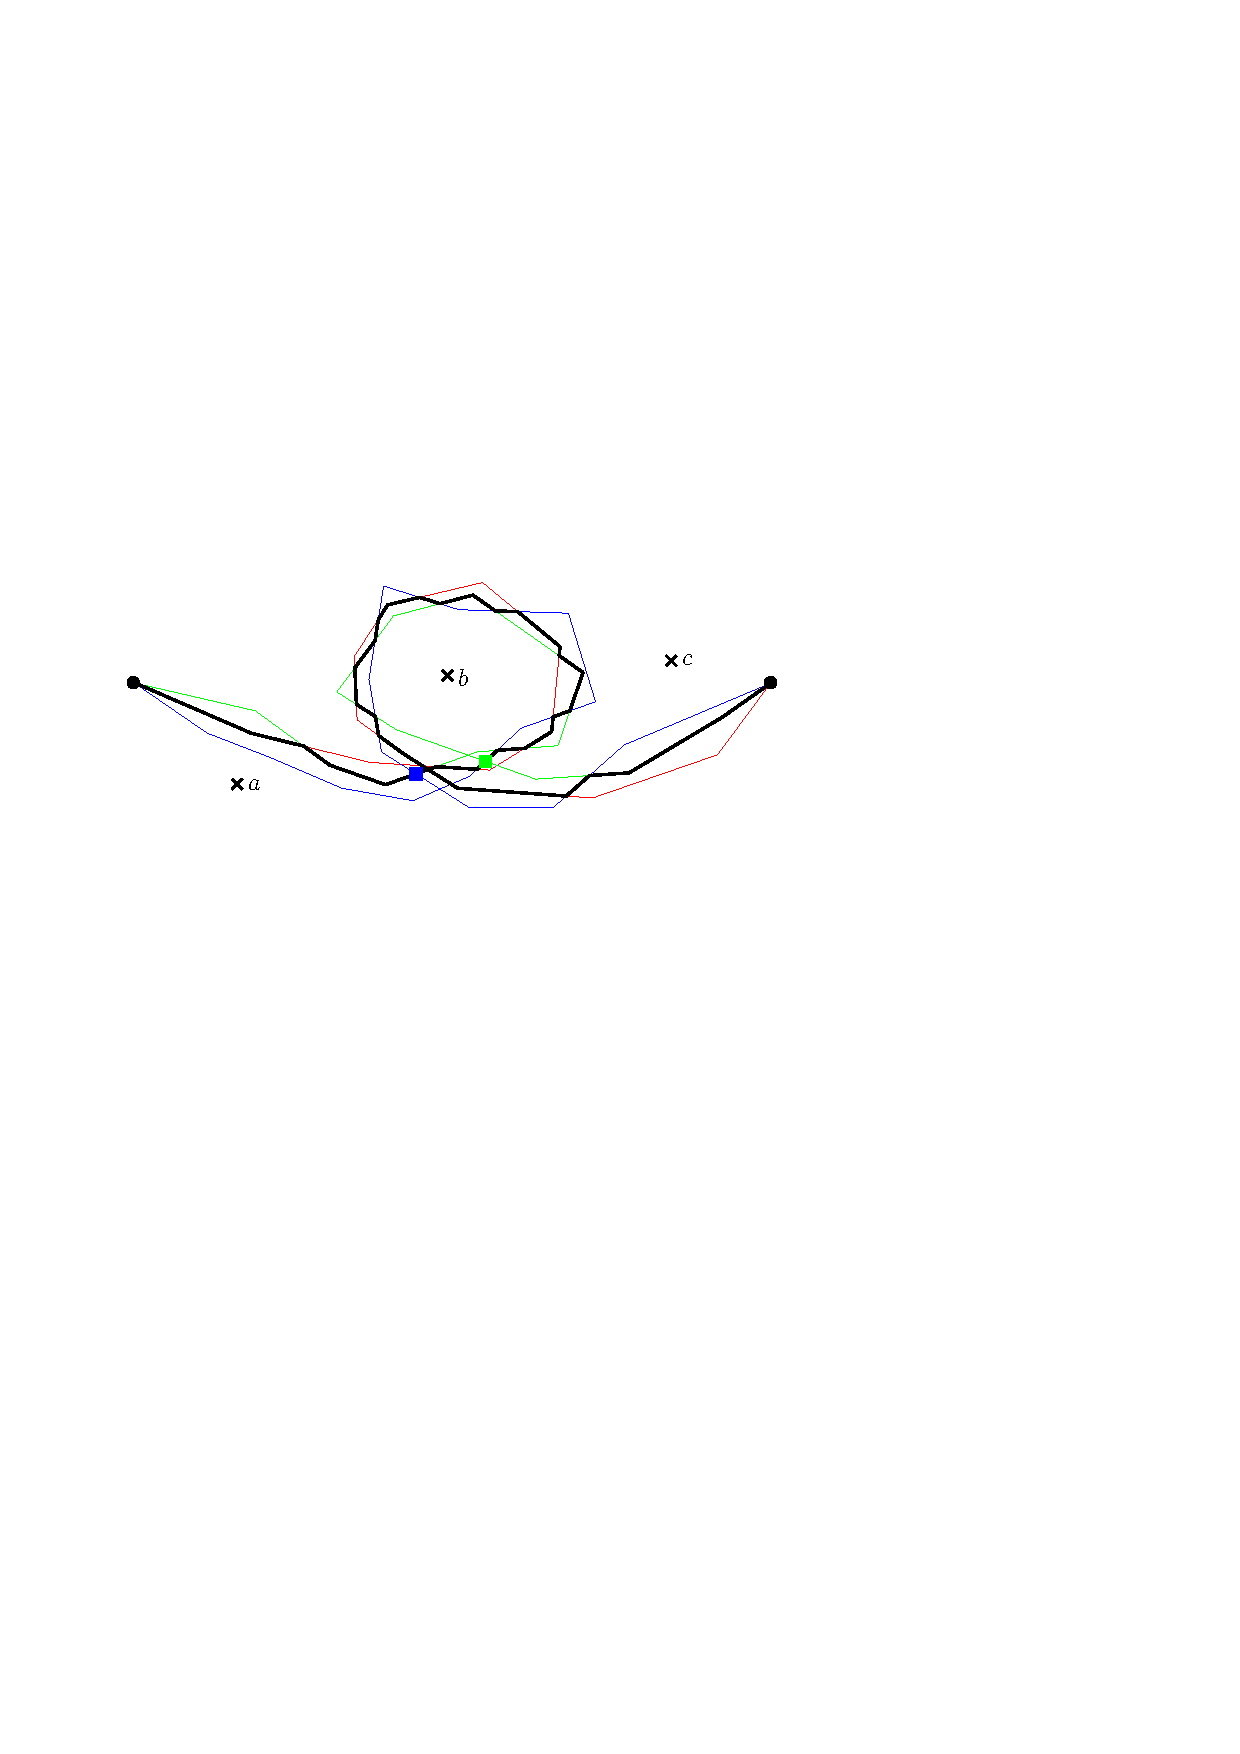
\includegraphics[scale=1]{Gambar/hmtp_works}
\caption[Modified switching method \cite{Lionov:2009}]{Modified switching method \cite{Lionov:2009}} 
\label{fig:homotopy_algo}
\end{figure}

If the median switches at this intersection, the final signature will be \textit{$a^{+}b^{-}c^{-}$}, which is not the signature of this set (\textit{$a^{+}b^{-}b^{+}b^{-}c^{-}$}). 
At this point, the median does not switch to another trajectory. 
Instead, it continues to move along the green trajectory. 
The same situation also occurs when the median (now following the blue trajectory) intersects with the green trajectory (at the small green square).

Although this algorithm can produce a more suitable median trajectory for the situation where the switching method fails, the quality of the homotopic median trajectory depends heavily on the following factors:
\begin{itemize}
\item placement of the crosses
\item the number of trajectories which have the same signature 
\end{itemize}

Therefore, in several cases the algorithm with the homotopy concept cannot produce suitable median trajectories.
We give two examples in Figure~\ref{fig:homotopy_fail0}: in the left-hand side of figure, the final median trajectory (blue) does not follow other trajectories to the area with a narrow space. 
This problem arises because that narrow space is not large enough for a cross to be placed. 

\begin{figure}
\centering
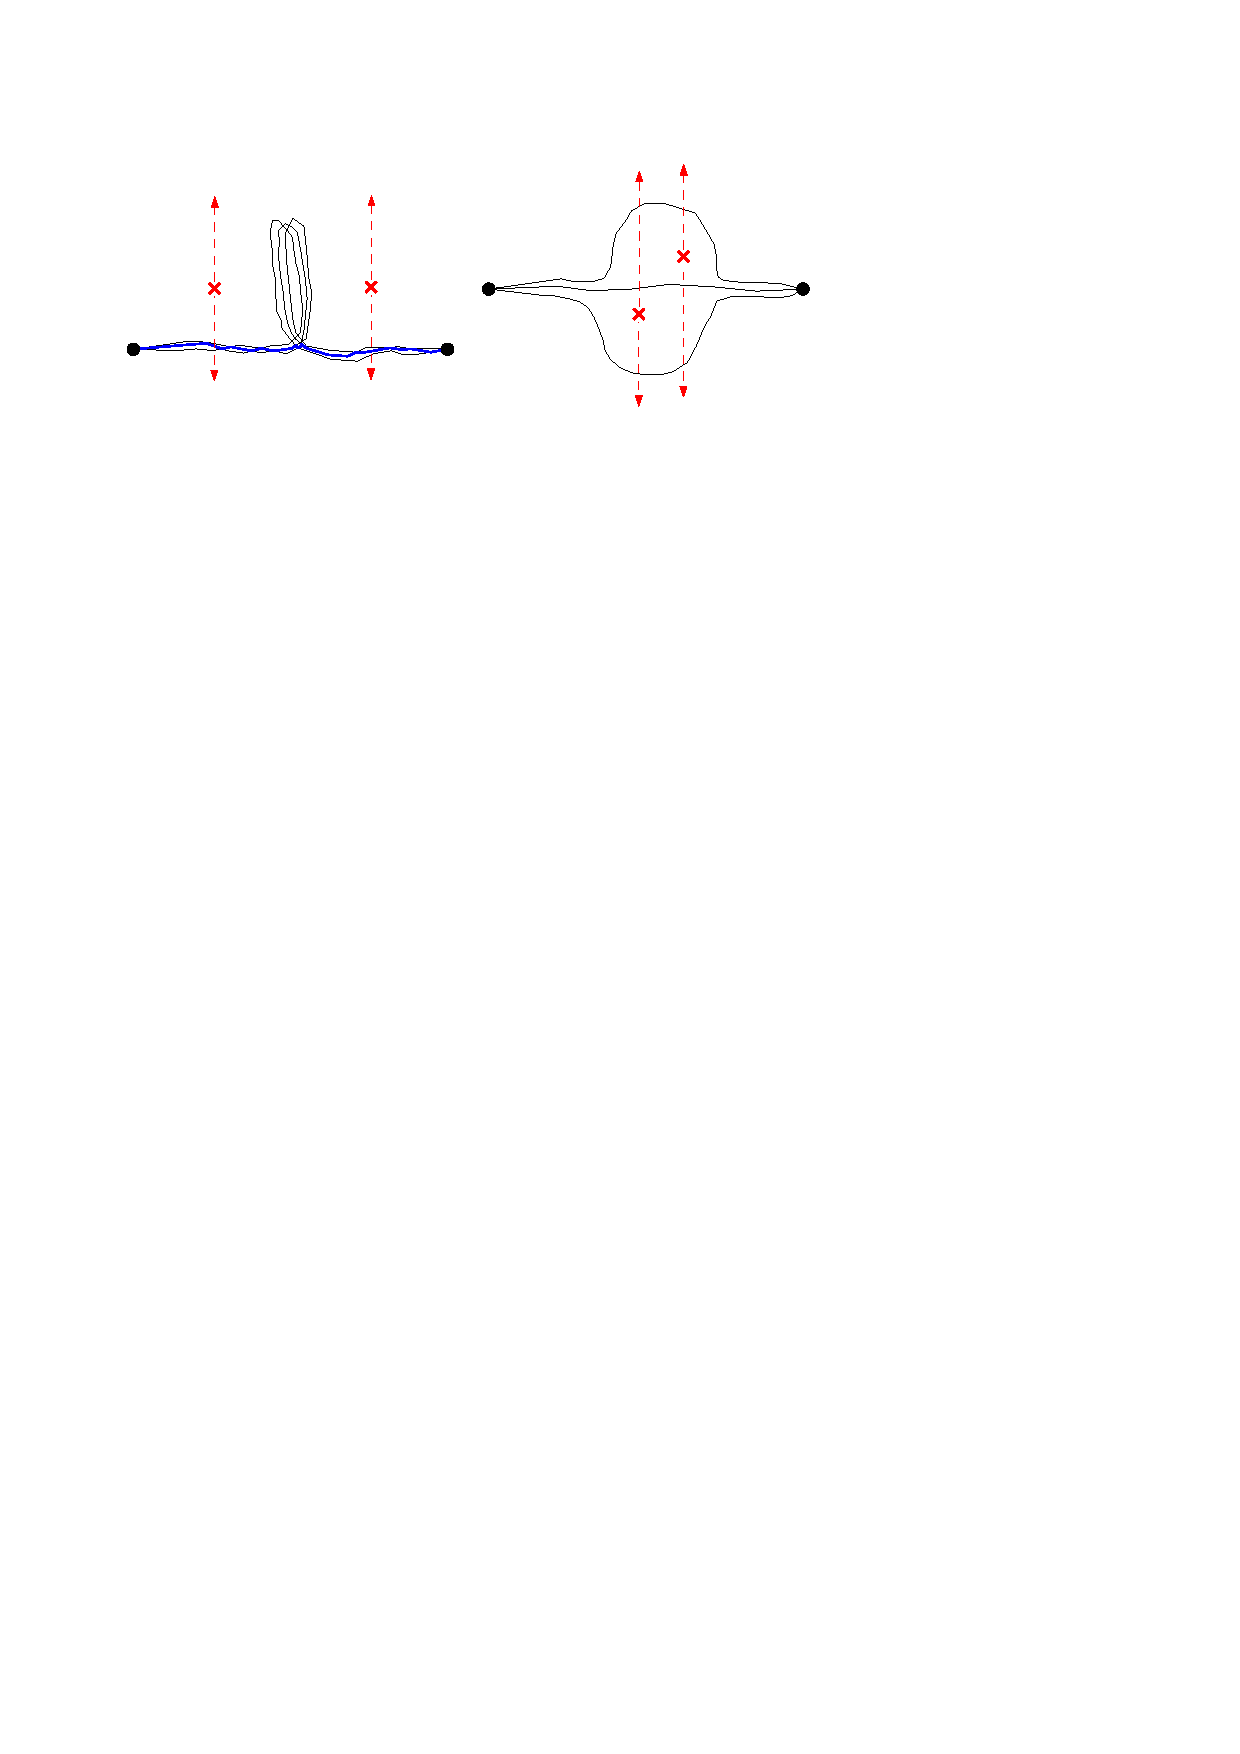
\includegraphics[scale=1]{Gambar/homotopy_fail0}
\caption[Example cases where algorithm using homotopy will fail]{Example cases where algorithm using homotopy will fail} 
\label{fig:homotopy_fail0}
\end{figure}

In the right-hand side of the figure, there are no two trajectories homotopically equivalent to each other. 
Nevertheless, by looking at their position, the median trajectory should be the one in the middle (between the two crosses).
However, the algorithm with the homotopy concept does not guarantee that a suitable median trajectory will be found because there is no subset that contains the majority of trajectories in $T$. 
Figure~\ref{fig:homotopy_fail1} shows an example from \cite{Lionov:2009}, where the median trajectory does not completely follow what other trajectories do.

\begin{figure}
\centering
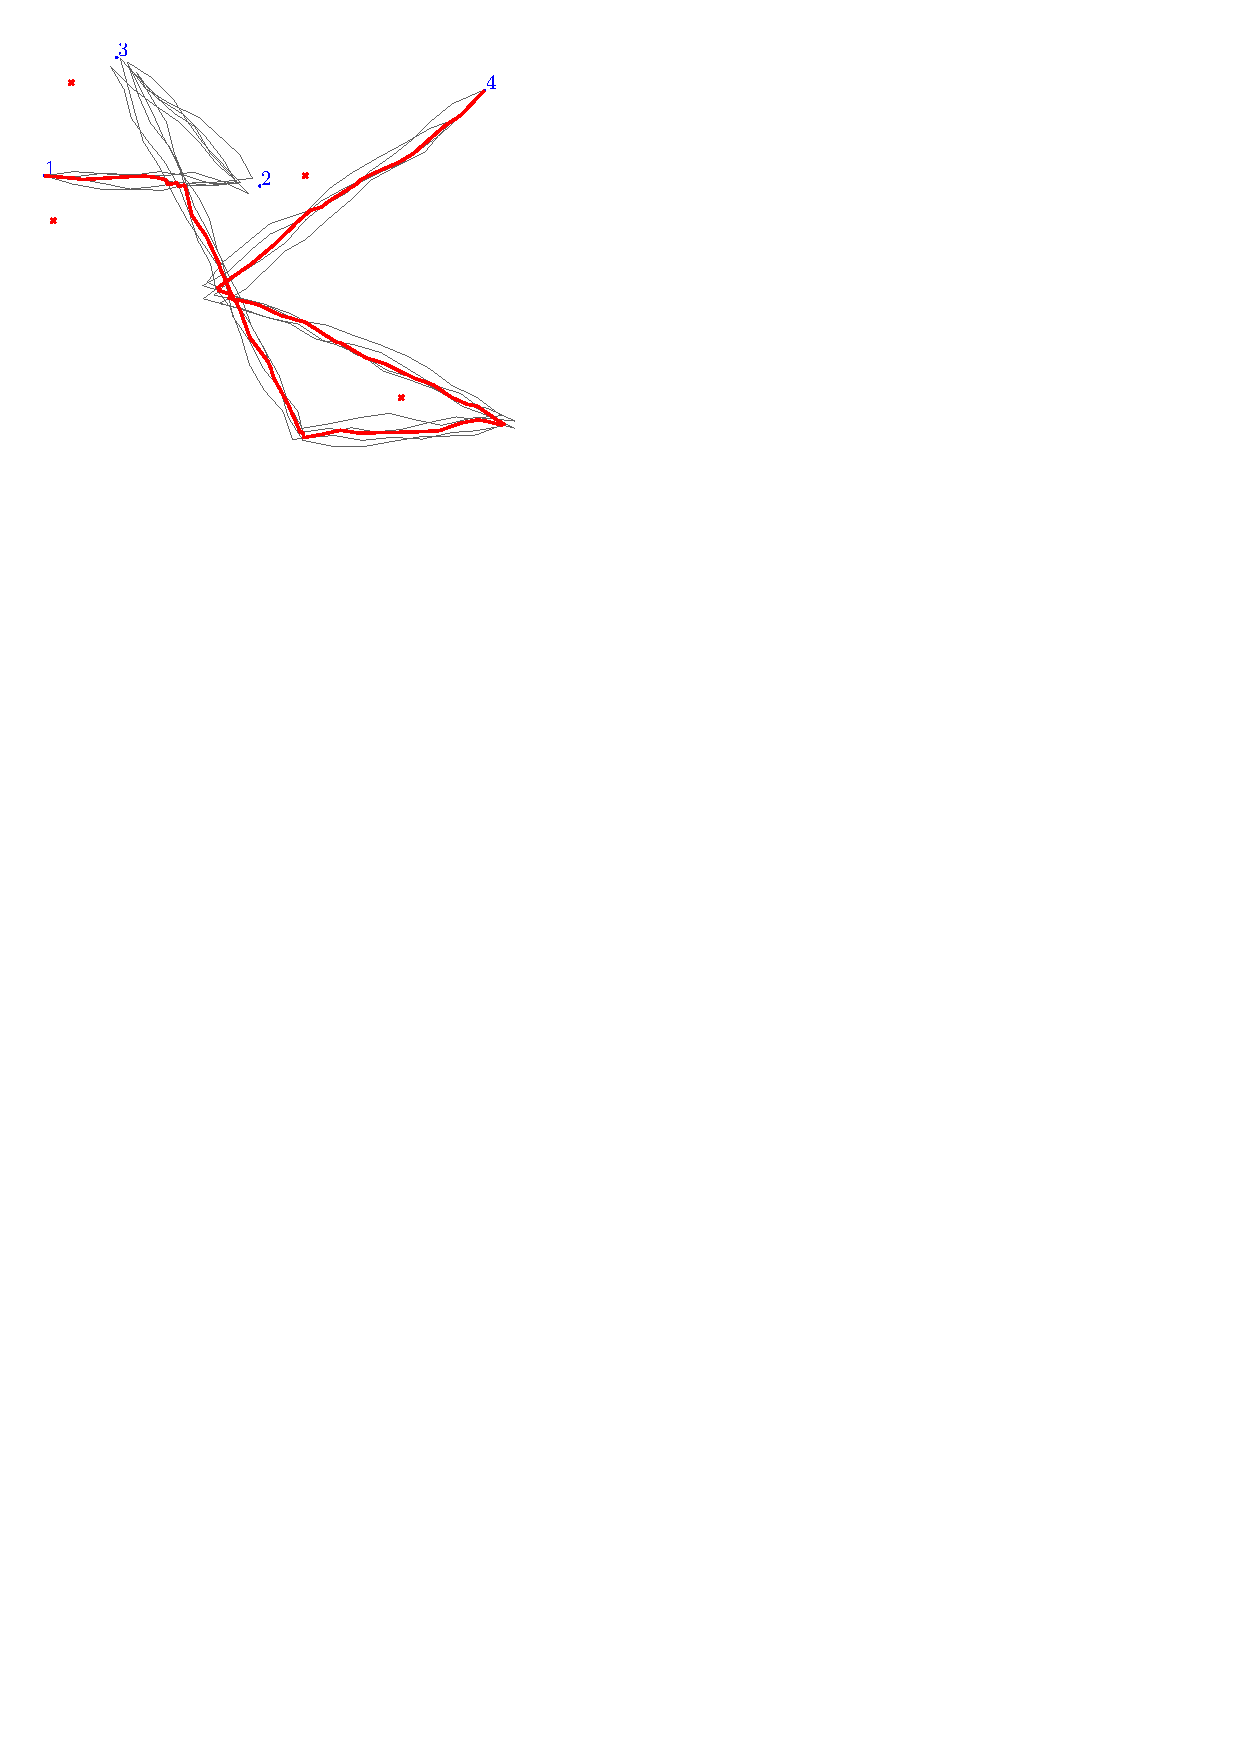
\includegraphics[scale=1]{Gambar/homotopy_fail1}
% \caption[The median trajectory does not pass through part of trajectories in the upper left area]{The median trajectory does not pass through part of trajectories in the upper left area} 
\caption{The median trajectory does not pass through part of trajectories in the upper left area}
\label{fig:homotopy_fail1}
\end{figure}

\subsection{The Proposed Solutions}
\label{sec:solution}

To solve the problems we mention in the previous section, we propose two algorithms to compute the median trajectory from a set of $m$ trajectories (where each trajectory has $n$ segments).

The first algorithm is an $O(1.2108^{m} + m^{5}n^{5})$ worst-case time algorithm.
This algorithm uses the Fr\'{e}chet Distance \cite{AltGodau:1995} and works similar to the algorithm using the homotopy concept because both of them have to create the largest subset of similar trajectories and then compute the median trajectory by using parts of trajectories in that subset. 
By using the Fr\'{e}chet Distance, we avoid the requirement to find proper places to put crosses, but still can produce suitable median trajectory in the situation where the homotopic algorithm fails (e.g. the example with a narrow space).

The second algorithm uses the combination of the buffer concept and Dijkstra's Shortest Path algorithm.
Unlike all previous algorithms, this algorithm does not need to find the largest subset consisting similar trajectories. 
% Thus, it will solve the second problem from the homotopy concept, where each trajectory is different from each other .
Using this algorithm, we can compute the median trajectory in $O(h^{2} \log h)$ time in the worst-case, where $h$ is the number of all segments in $T$ $(h = O(mn))$.

We implemented the second algorithm in Java programming language and experiments have been done to determine the quality of the resulting median trajectory produced by this algorithm.
To provide the test data (set of trajectories), we use a trajectories generator instead of using real-world data.
This allow us to test much larger sets of trajectories

\section{Outline of the Thesis}
\label{sec:outline}

Chapter \ref{chap:definition} describes the properties for a set of trajectories and also some properties the median trajectory should have.

The next two chapters explain in detail the two algorithms:
\begin{itemize}
\item 
Chapter 3 starts with a brief introduction of the Fr\'{e}chet Distance and after that, we will explain how to use it to compute the median trajectory. 
\item 
Chapter 4 introduces the method to compute the median trajectory using the combination of the buffer concept and Dijkstra's shortest path algorithm. 
\end{itemize}

We will give an explanation about our implementation, particularly on the implementation of the trajectories generator, in Chapter 5.
In Chapter 6, we present the measures used to evaluate the quality of the median trajectory, the experiments set-up and the results from the experiments.
This thesis will be concluded in Chapter 7 and 8, where we draw conclusions and discuss some issues and possible directions for further research.

\lipsum[1-14]}{}
\ifdefstring{\vbabb}{1}{\chapter{The Description of a Set of Trajectories and Its Median Trajectory}
\label{chap:definition}

\section{Set of Trajectories}
\label{sec:setoftrjs}

In this thesis, we only consider the spatial component of the trajectory. 
Therefore, we represent a trajectory as a polygonal line built by a series of points and connected by line segments.   
 
Let $T:=\{\tau_{1},\tau_{2},...,\tau_{m}\}$ be the input set of $m$ trajectories for which we want to compute its median trajectory $\tau^{M}$.
We define each trajectory in $T$ as a list of at most $n$ points, $\tau_{i}:=(p_{i,1},...,p_{i,k})$ where $1 \leq i \leq m$ and $2 \leq k \leq n$. 
Note that the number of points for each trajectory can be different.
Every two consecutive points $p_{i,j}$ and $p_{i,j+1}$ $(1 \leq j \leq k-1)$ are connected by a segment $s_{i,j}:=(\overline{p_{i,j},p_{i,j+1}})$.

$P$ is the set of all points in $T$, $P:=\{p_{i,j} \mid i \in \{ 1 ... m\} , j \in \{ 1 ... n\} \}$ and $S$ is the set of all segments in $T$, $S:=\{s_{i,j} \mid i \in \{ 1 ... m\} , j \in \{ 1 ... n-1\} \}$.
All trajectories in $T$ share the same start and end points $(p_{1,1}=p_{2,1}=...=p_{m,1}$ and $p_{1,k_{1}}=p_{2,k_{2}}=...=p_{m,k_{m}}$ where $ \{k_{1},...,k_{m}\} \in \{1,...,n\})$. 

Trajectories can intersect with other trajectories in other points than their start and end points.
These intersection points are also included in the list of points that define the trajectory. When two segments intersect each other, then both segments will be split into two parts and all four segments share one intersection point as one of their endpoints (see Figure~\ref{fig:number_trj}).

\begin{figure}
\centering
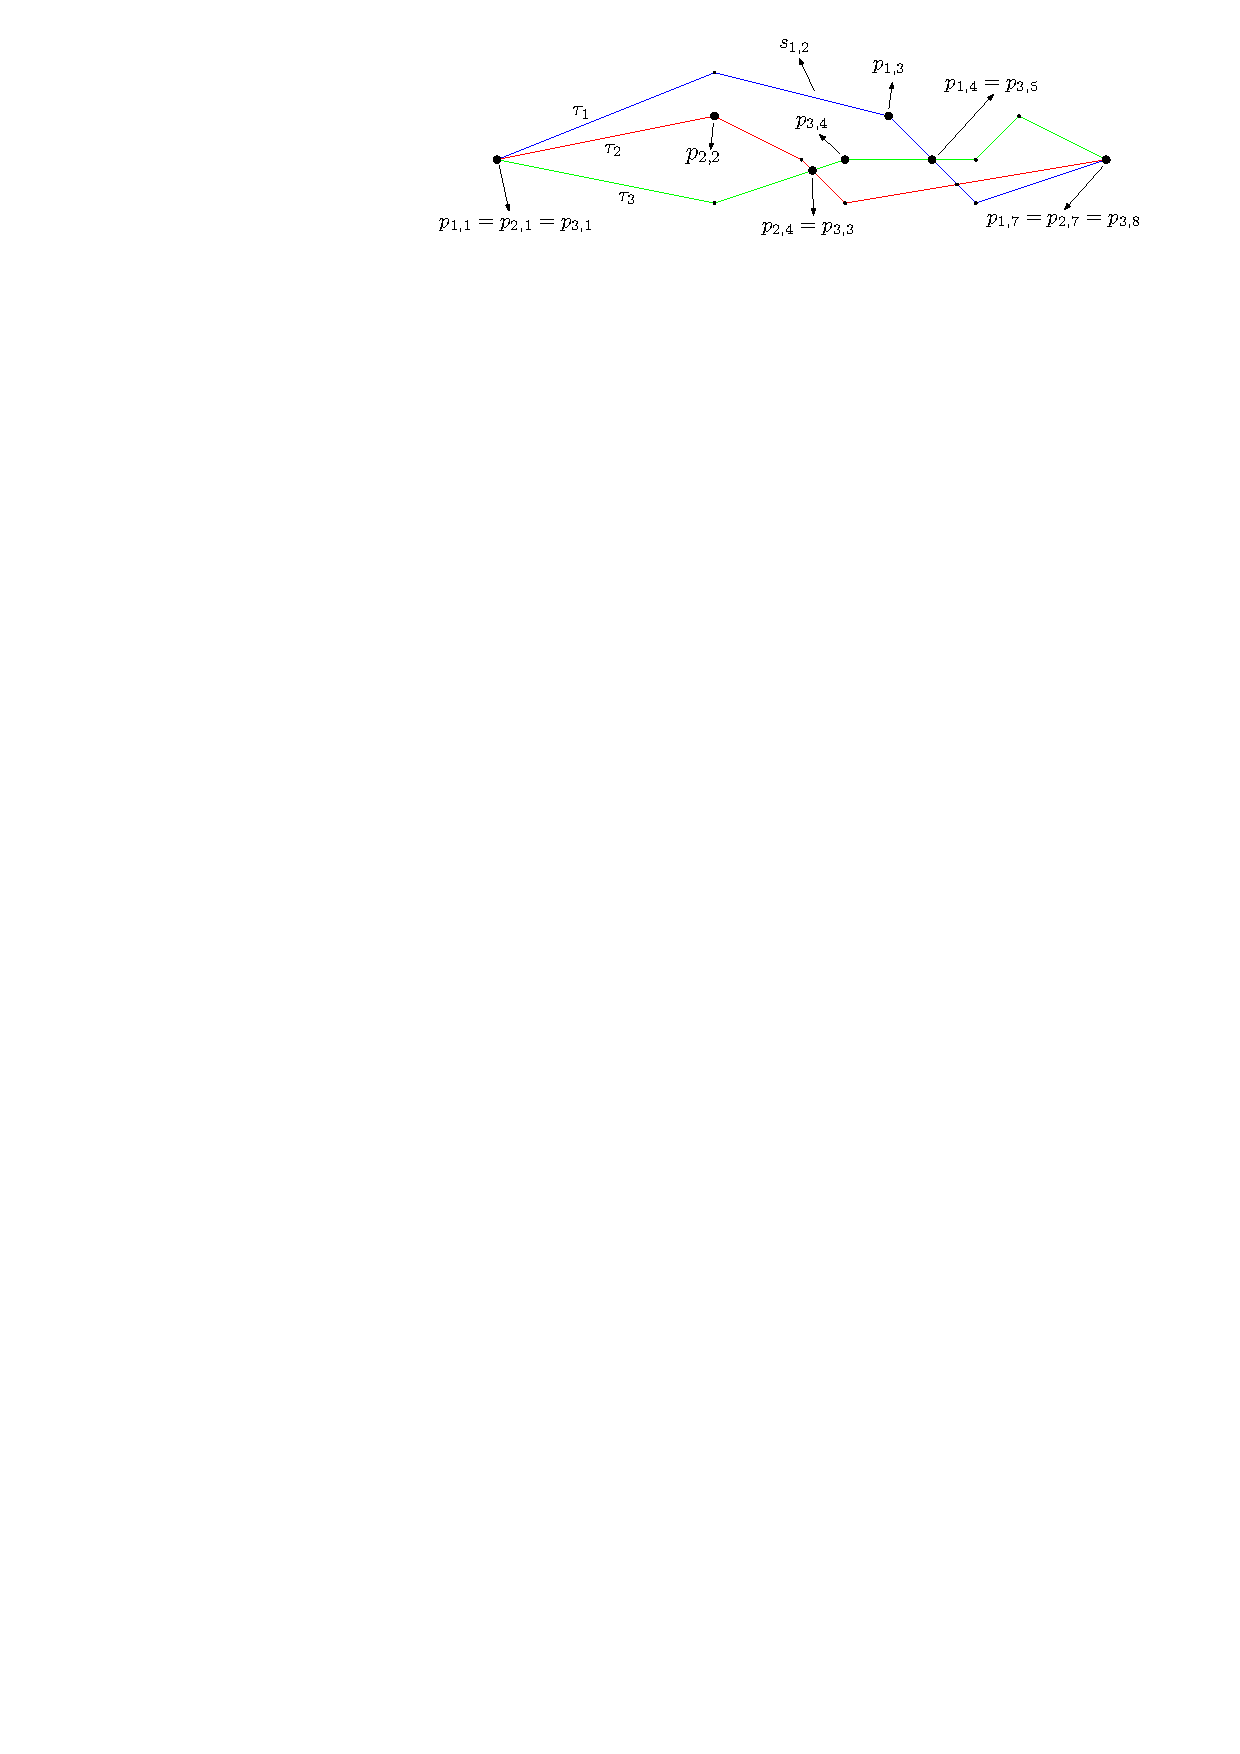
\includegraphics[scale=0.8]{Gambar/number_trj}
\caption[Numbering of points and segments]{Numbering of points and segments} 
\label{fig:number_trj}
\end{figure}

Let $n'$ be the number of points in a trajectory, including their intersection points with other trajectories. 
In the worst case, $n' = mn^{2}$. 
In the rest of this thesis, we define $n$ as a number of points in a trajectory, inclusive with its intersection points with other trajectories. 
Note that the number of segments for each trajectory is linear to the number of points, because trajectory with $n$ points has $n-1$ segments.

\section{Properties of the Median Trajectory}
\label{sec:prop_medtrj}

We define several properties for the median trajectory  $\tau^{M}$ with respect to the input set of trajectories $T$:

\begin{itemize}
\item 
$\tau^{M}$ is a directed polygonal line from start point to end point and should be similar to most trajectories in $T$.

\item 
It must be built only using points and segments which are parts of trajectories in the input set. 

\item 
The usage of segments should follow the direction of them. Therefore, it is not allowed to use a segment such that the direction of $\tau^{M}$ is opposite to the direction of that segment in a trajectory (see Figure~\ref{fig:forbid_seg}, indicated by the dark blue arrow).

\begin{figure}
\centering
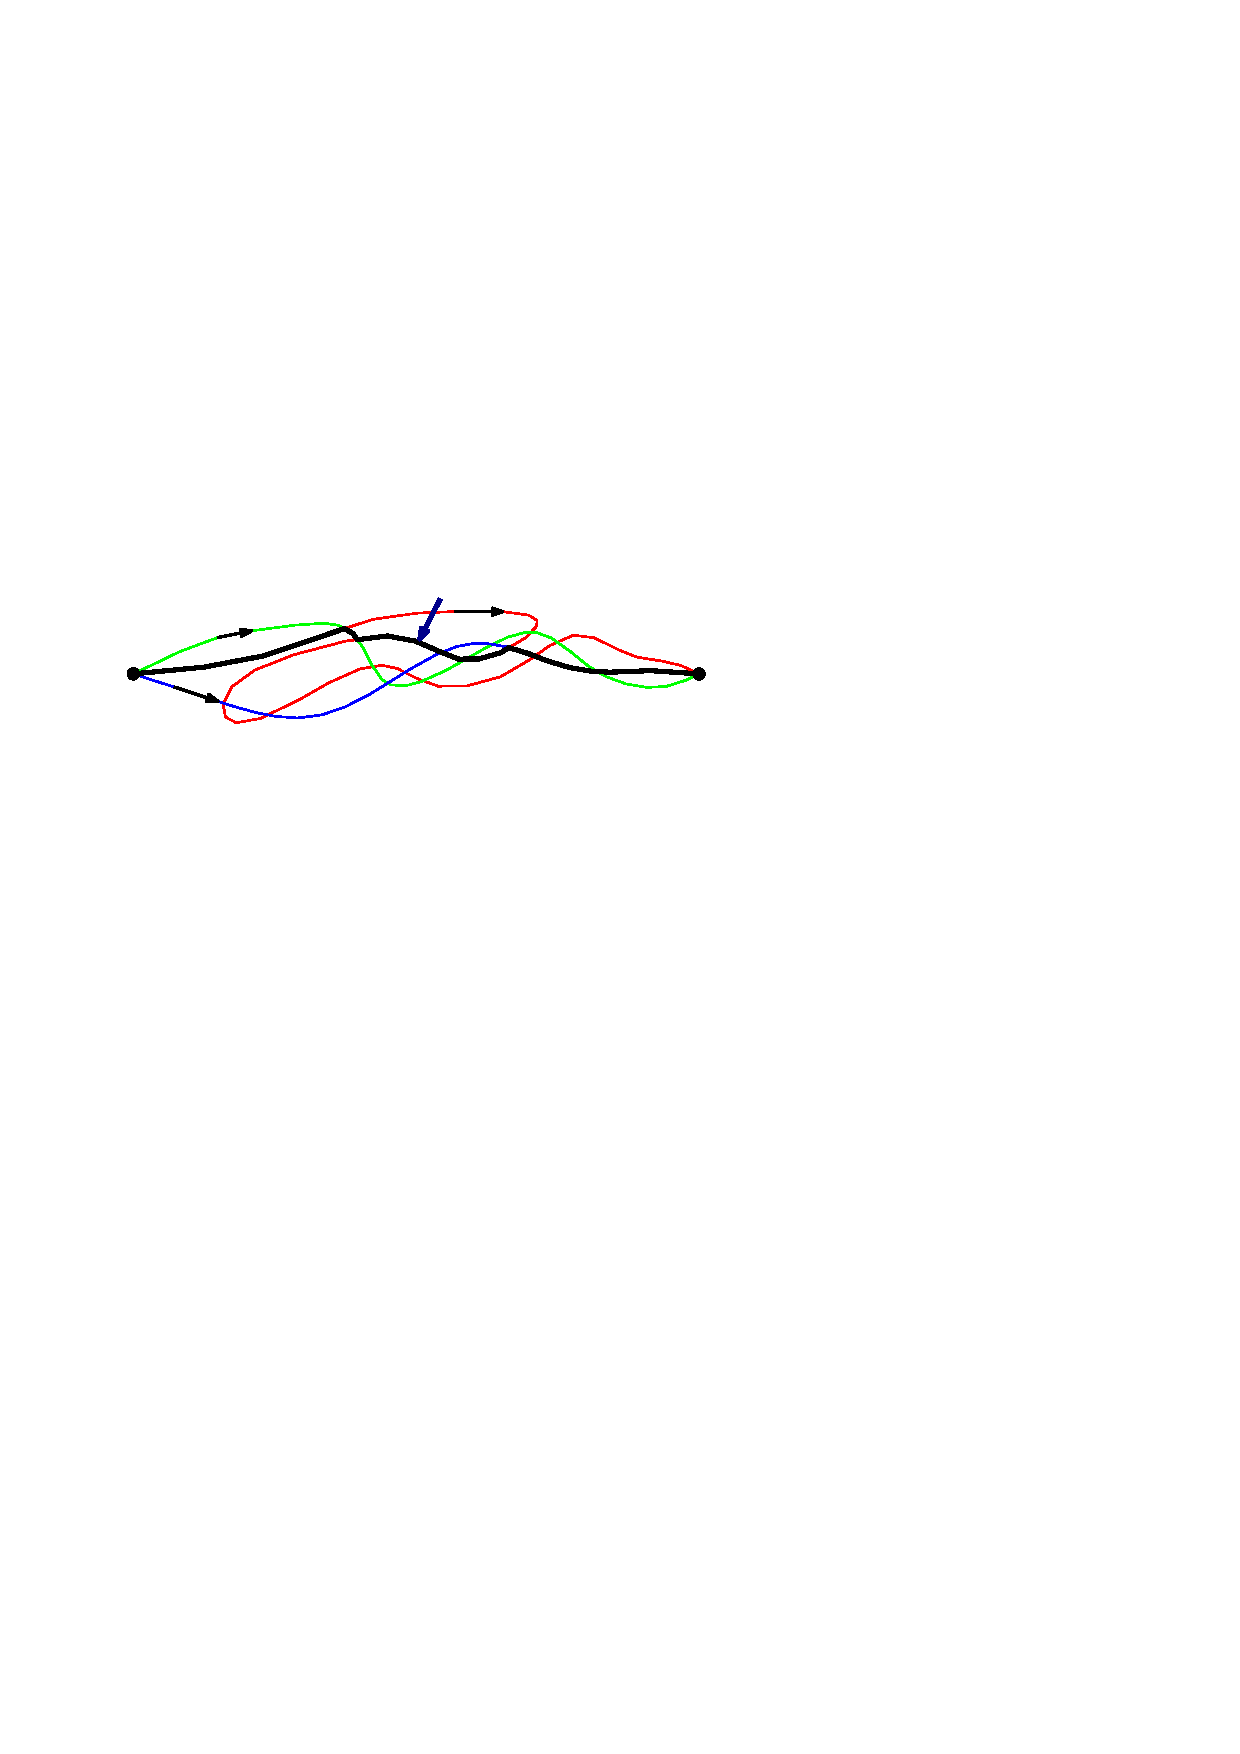
\includegraphics[scale=0.9]{Gambar/forbid_seg}
\caption[Possible median trajectory (in black) with backward direction (pointed by the blue arrow)]{Possible median trajectory (in black) with backward direction (indicated by the blue arrow)} 
\label{fig:forbid_seg}
\end{figure}

\item 
The length of the median trajectory should be relatively the same as the average length of all trajectories in the input set.

\item 
The total angular change should also be similar to the average of total angular change of all trajectories in the input set.
The total angular change of a trajectory is the sum of all angular changes at every vertex in that trajectory (see Figure~\ref{fig:total_ang}). 

\begin{figure}
\centering
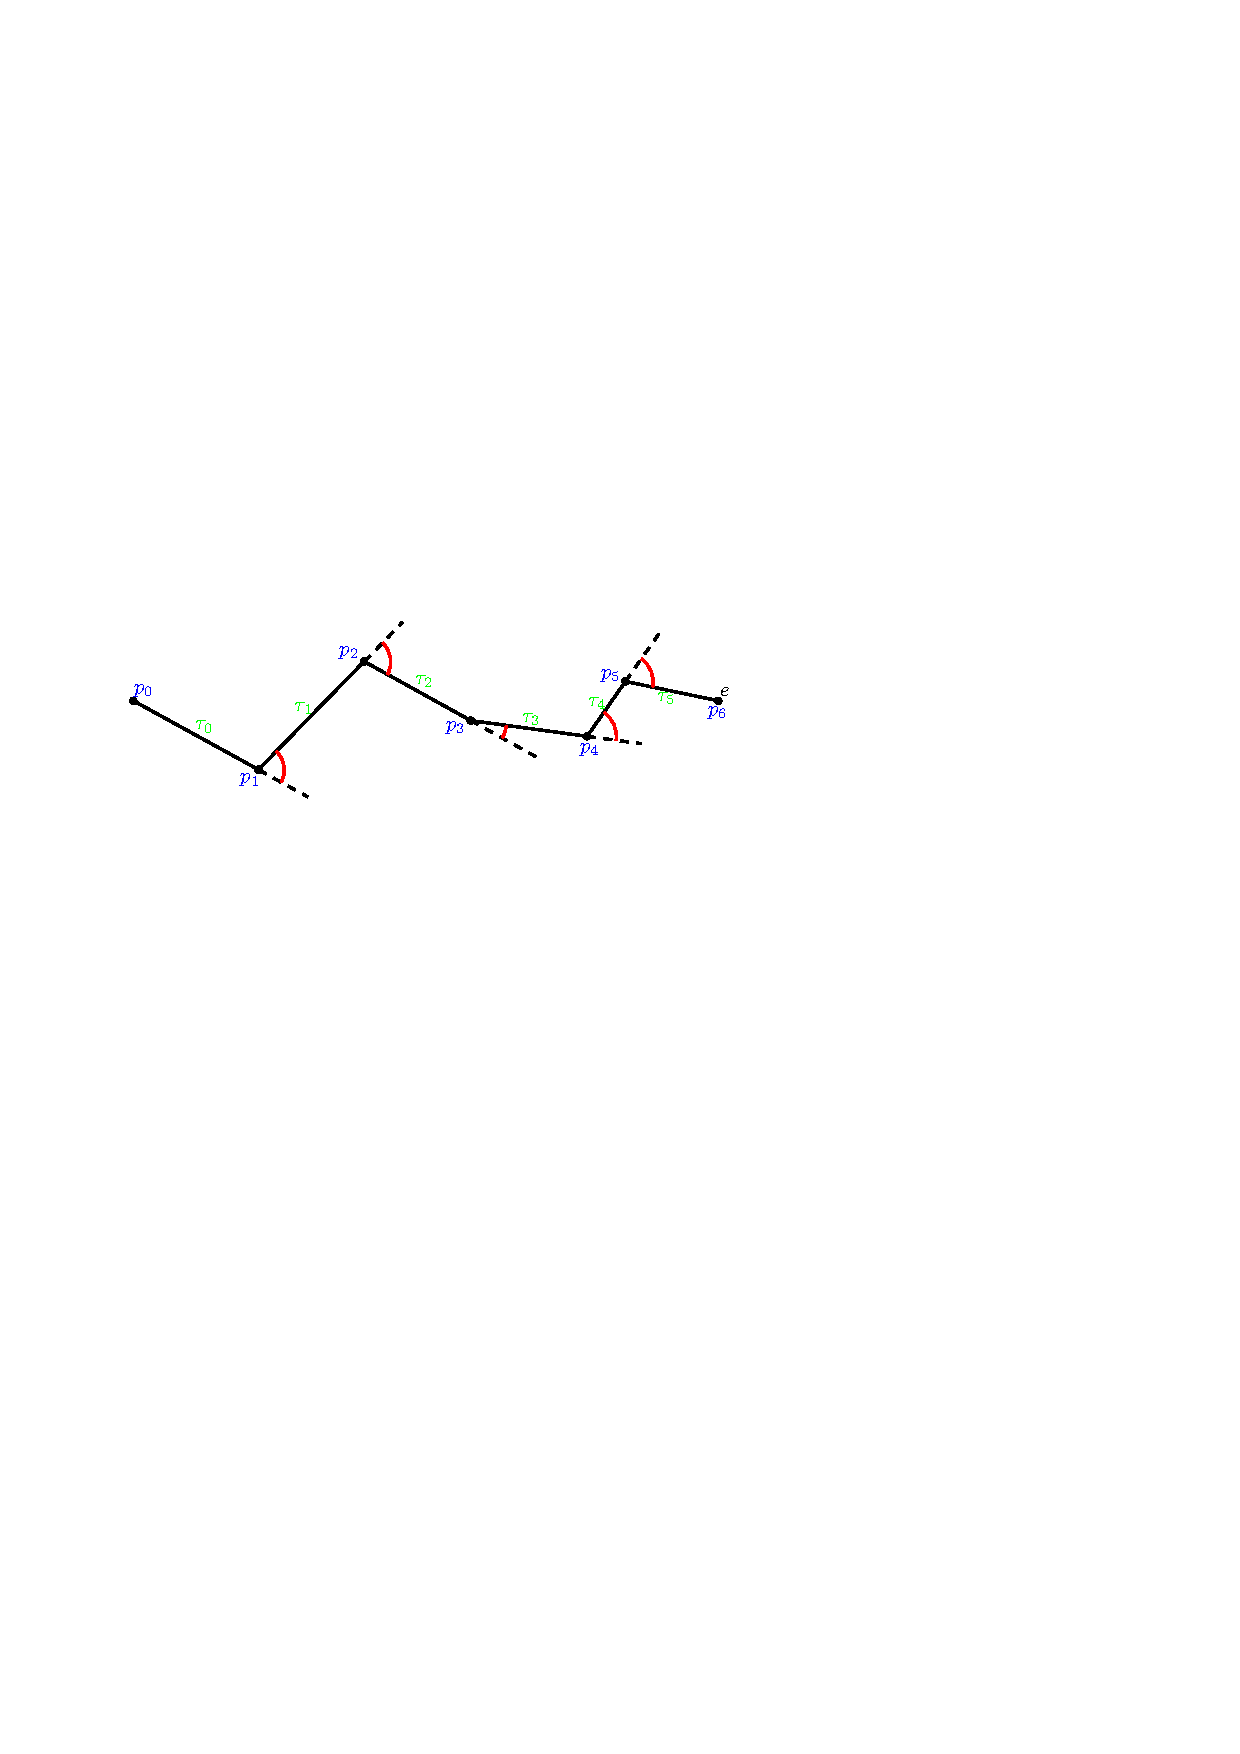
\includegraphics[scale=1]{Gambar/total_ang}
\caption[Red arcs indicate the angular change at each vertex]{Red arcs indicate the angular change at each vertex} 
\label{fig:total_ang}
\end{figure}

\item 
The number of vertices and edges of $\tau^{M}$ should be about the same with the average of the number of vertices and edges from all trajectories in the input set.
		%\item The final result of $\tau^{M}$ should not be influenced by an outliers.  
\end{itemize}


Using the definition of the input set of trajectories defined in the previous section, we define a median trajectory $\tau^{M}$ as a sequence of points from $T$, $\tau^{M}:=(p_{i_{1},j_{1}},p_{i_{2},j_{2}},...,$ $p_{i_{k},j_{k}})$ where $\{i_{1},i_{2},...,i_{k}\} \in \{1 ... m\}$ and $\{j_{1},j_{2},...,j_{k}\} \in \{ 1 ... n\}$, or defined as a sequence of segments: $\tau^{M}:=(s_{i_{1},j_{1}},s_{i_{2},j_{2}}, ...,s_{i_{k},j_{k}})$ where $\{i_{1},i_{2},...,i_{k}\} \in \{1 ... m\}$ and $\{j_{1},j_{2},...,j_{k}\} \in \{1 ... n-1\}$. 
Note that $\tau^{M}$ and all trajectories in $T$ share the same start point and end point.   


%  

Table~\ref{tab:tab_begin} shows how this information is kept in $\Gamma$. 
\begin{table}
\centering
\caption{Table $\Gamma$ after inserting $\mathcal{S}_{1}$}
\label{tab:tab_begin}
\begin{tabular}{cccc}
\toprule

 & $v_{start}$ & $\mathcal{S}_{1}$ & $v_{end}$\\
\midrule
$\tau_{1}$ & 1 & 12& 20\\
$\tau_{2}$ & 1 &  & 20\\
$\tau_{3}$ & 1 & 9 & 20\\
$\tau_{4}$ & 1 &  & 20\\
\bottomrule
\end{tabular}
\end{table}

There are two possibilities of the placement of $\mathcal{S}_{2}$: 
\begin{table}[H]
\begin{minipage}[c]{0.49\linewidth}
\centering
\caption{$\mathcal{S}_{2}$ between $v_{start}$ and $\mathcal{S}_{1}$}
\label{tab:tab_next1}
\begin{tabular}{ccccc}
\toprule

 & $v_{start}$ & $\mathcal{S}_{2}$ & $\mathcal{S}_{1}$ & $v_{end}$\\
\midrule
$\tau_{1}$ & 1 & 5 \cellcolor{green}& 12& 20\\
$\tau_{2}$ & 1 & 8 \cellcolor{green}& & 20\\
$\tau_{3}$ & 1 & 2/8/17 \cellcolor{green}& 9 & 20\\
$\tau_{4}$ & 1 & \cellcolor{red}& & 20\\
\bottomrule
\end{tabular}
\end{minipage}
\begin{minipage}[c]{0.49\linewidth}

\centering
\caption{$\mathcal{S}_{2}$ between $\mathcal{S}_{1}$ and $v_{end}$}
\label{tab:tab_next2}
\begin{tabular}{ccccc}
\toprule

 & $v_{start}$ & $\mathcal{S}_{1}$ & $\mathcal{S}_{2}$ & $v_{end}$\\
\midrule
$\tau_{1}$ & 1 & 12& 5 \cellcolor{red} &20\\
$\tau_{2}$ & 1 &  &  8 \cellcolor{green} &20\\
$\tau_{3}$ & 1 & 9 & 2/8/17 \cellcolor{green} &20\\
$\tau_{4}$ & 1 &   & \cellcolor{red} &20\\
\bottomrule
\end{tabular}
\end{minipage}
\end{table}

The final placement of table $\Gamma$ after simplification: 
\begin{table}[H]
\centering
\caption{Final $\Gamma$}
\label{tab:tab_final}
\begin{tabular}{ccccc}
\toprule
 & $v_{start}$ & $\mathcal{S}_{2}$ & $\mathcal{S}_{1}$ & $v_{end}$\\
\midrule
$\tau_{1}$ & 1 & 5 & 12& 20\\
$\tau_{2}$ & 1 & 8 &   & 20\\
$\tau_{3}$ & 1 & 8 & 9 & 20\\
$\tau_{4}$ & 1 &   &   & 20\\
\bottomrule
\end{tabular}
\end{table}

}{}
\ifdefstring{\vbabc}{1}{\chapter{Analisis}
\label{chap:analisis}

Pada bab ini akan dijelaskan analisis mengenai hasil wawancara, hasil kuesioner, nama baptis berdasarkan metode SAW, nama baptis berdasarkan metode SAW menggunakan database, dan perangkat lunak berupa \textit{use case}.

\section{Analisis Hasil Wawancara}
\label{sec:analisiswawancara}

Dalam menganalisis kebutuhan pemilihan nama baptis Katolik, peneliti melakukan wawancara dengan Pastor Paroki St. Laurentius, A. Boogaarts, OSC (Lampiran \ref{fig:bukti}). Wawancara dengan Pastor Paroki bertujuan untuk mengetahui secara mendetail atau terperinci mengenai pembaptisan dalam agama Katolik. Setelah melakukan wawancara, penulis mendapatkan penjelasan secara umum mengenai Baptis, nama Baptis, serta cara pemilihan nama Baptis.
\begin{enumerate}
	\item Makna baptis untuk agama Katolik adalah suatu lambang lahiriah di mana diungkapkan, bahwa menjadi anggota gereja Katolik yang secara resmi adalah diangkat menjadi anak Allah.
	\item Tidak harus ada nama baptis. Tetapi nama baptis merupakan suatu tradisi sebagai ungkapan bahwa di dalam baptisan itu dikuduskan dengan harapan tidak sembarangan memilih nama baptis, tetapi lebih ingin meniru teladan orang kudus yang dia pilih sebagai nama baptis, sehingga menjadi kudus dengan nama baptis yang dia pilih.
		%\item Cara pembaptisan dalam agama Katolik selain disiram dengan air adalah ditenggelamkan/ dibenamkan/ dicelupkan menggunakan air yang mengalir yang telah diberkati (air percikan tidak cukup).
		%\item Ada beberapa kelemahan ketika baptis waktu bayi, yaitu kurangnya mendapatkan pendalaman iman. Tetapi ada keuntungannya juga, yaitu telah mengikut Yesus Kristus dari sewaktu Bayi. Sedangkan jika baptis dewasa, yaitu benar-benar belajar dengan cara mencari komunitas/ dapat membantu dia memilih Yesus Kristus sebagai Juru Selamat serta Kitab Suci dan sebagainya.
		\item Pemilihan nama baptis tidak ada kriteria (bebas memilih), tetapi sebaiknya kita memilih orang yang sekiranya dekat dengan bakat kita/ nama karena mirip/ karena artinya. Tanggal, tanggal pembaptisan serta pesta nama baptis juga bisa dijadikan acuan dalam memilih nama baptis.
\end{enumerate}

		Penelitian ini berfokus pada pembahasan pemilihan nama baptis, untuk itu bagian yang akan dianalisa lebih mendalam adalah pada bagian kriteria pemilihan nama Baptis. Berdasarkan hasil wawancara di atas, dapat dianalisa bahwa nama baptis tidak diharuskan, tetapi nama baptis sudah merupakan sebuah tradisi dalam agama Katolik. Kriteria pemilihan nama baptis yang bisa dijadikan sebuah acuan atau pedoman dalam memilih nama Baptis berdasarkan hasil wawancara adalah sebagai berikut:
	
	\begin{itemize}
		\item Bakat calon Baptis (profesi)
		\item Nama calon Baptis
		\item Tanggal lahir calon Baptis
		\item Tanggal pembaptisan calon Baptis
		\item Tanggal Pesta santo-santa (tanggal peringatan)
		\item Arti santo-santa
	\end{itemize}


\section{Analisis Hasil Kuesioner}
\label{sec:analisiskuesioner}

Dalam menganalisis kebutuhan pemilihan nama baptis Katolik, peneliti menyebarkan kuesioner yang telah dibuat dengan menggunakan Google Form. Pada Google Form, terdapat lima pertanyaan. Berikut adalah pertanyaan dari formulir kuesioner pemilihan nama baptis Katolik (Lampiran \ref{fig:form}).


\begin{enumerate}
	\item Apakah anda seorang Katolik?
	
	Pertanyaan ini dibuat dengan tujuan agar penulis dapat mengetahui persentase \textit{user} yang mengisi beragama Katolik atau calon Katolik. Yang dimaksud calon Katolik adalah orang yang ingin masuk ke dalam agama Katolik atau mengikuti Kristus sebagai Juru Selamat-Nya. Penulis memberikan sebuah pilihan untuk jawaban pertanyaan ini, yaitu ya dan tidak. Jika \textit{user} mengisi dan jawabannya adalah ya, maka \textit{user} dapat membantu dalam hal analisis kebutuhan pemilihan nama baptis. %Jika \textit{user} mengisi dan jawabannya adalah Tidak, maka \textit{user} dapat menambah pengetahuan \textit{user} mengenai pemilihan nama baptis. 
	\item Jika jawaban anda Ya, apakah anda sudah dibaptis?
	
	Pertanyaan ini dibuat dengan tujuan agar penulis dapat mengetahui persentase \textit{user} yang sudah dibaptis. Penulis memberikan sebuah pilihan untuk jawaban pertanyaan ini, yaitu sudah dan belum. Jika \textit{user} mengisi dan jawabannya adalah sudah, maka \textit{user} dapat membantu dalam hal analisis kebutuhan pemilihan nama baptis. %Jika penulis sudah mengetahui presentasi yang dibaptis, maka dapat membantu dalam hal analisis kebutuhan pemilihan nama baptis.
	\item Jika sudah, kapan anda telah dibaptis?
	
	Pertanyaan ini dibuat dengan tujuan agar penulis dapat mengetahui persentase \textit{user} yang sudah dibaptis ketika bayi dan juga ketika dewasa. Penulis memberikan sebuah pilihan untuk jawaban pertanyaan ini, yaitu ketika masih bayi dan ketika sudah dewasa.
	%\item Apa yang membuat anda dibaptis?
	
	%Pertanyaan ini dibuat dengan tujuan agar penulis dapat mengetahui alasan yang membuat \textit{user} ingin dibaptis. Jawaban pertanyaan ini berupa teks kosong, sehingga \textit{user} dapat mengisi beberapa alasan secara bebas.
	\item Anda memilih nama baptis tersebut berdasarkan apa saja?
	
	Pertanyaan ini dibuat dengan tujuan agar penulis dapat mengetahui faktor yang patut untuk dijadikan sebagai sebuah kriteria pemilihan nama baptis Katolik. Penulis memberikan beberapa pilihan untuk jawaban pertanyaan ini, yaitu tanggal lahir, tanggal pembaptisan Anda, deskripsi santo-santa (cerita kehidupan santo-santa), tanggal pesta santo-santa (peringatan), profesi santo-santa, arti nama dari santo-santa, lambang dari santo-santa, dan jika \textit{user} ingin menjawab selain pilihan tersebut. Jawaban dengan pilihan yang lain juga dapat dijadikan sebuah kriteria, jika jawabannya masuk akal.
\end{enumerate}

Penelitian ini berfokus pada pembahasan pemilihan nama baptis, untuk itu bagian yang akan dianalisa lebih mendalam adalah pada bagian kriteria pemilihan nama Baptis. Sampel yang diambil adalah seratus orang yang terdiri dari 96 orang beragama Katolik dan 4 orang calon Katolik (Lampiran \ref{fig:kues1}, Lampiran \ref{fig:kues2}, Lampiran \ref{fig:kues3}, Lampiran \ref{fig:kues4}, Lampiran \ref{fig:kues5}, Lampiran \ref{fig:kues6}). Setiap responden ada yang memilih kriteria nama baptis sampai 4 atau 5 kategori. Kriteria pemilihan nama baptis yang bisa dijadikan sebuah acuan atau pedoman dalam memilih nama Baptis berdasarkan hasil kuesioner adalah sebagai berikut (Gambar \ref{fig:Capture}):

\begin{itemize}
			\item Tanggal Lahir sebanyak 11 \textit{user}.
			\item Tangal Pembaptisan sebanyak 6 \textit{user}.
			\item Deskripsi atau cerita kehidupan Santo-Santa sebanyak 32 \textit{user}.
			\item Pesta Santo-Santa sebanyak 1 \textit{user}.
			\item Profesi Santo-Santa sebanyak 6 \textit{user}.
			\item Arti Nama Santo-Santa sebanyak 45 \textit{user}.
			\item Lambang dari Santo-Santa sebanyak 5 \textit{user}.
			\item Lain-lain sebanyak 26 \textit{user}.
		\end{itemize}
		
	\begin{figure}[htbp]
		\centering
			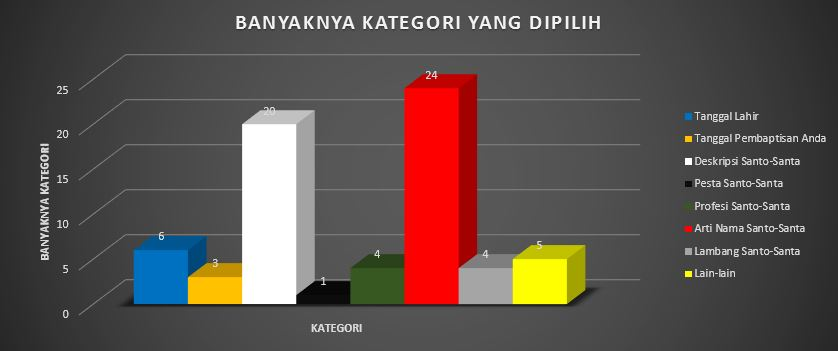
\includegraphics[scale=0.7]{Gambar/Capture.JPG}
			\caption{Kategori Pemilihan Nama Baptis}
		\label{fig:Capture}
	\end{figure}

	Dengan demikian, berdasarkan hasil kuesioner di atas (Gambar \ref{fig:Capture}), dapat di analisa bahwa kriteria yang paling banyak dijadikan acuan atau pedoman (diurutkan berdasarkan responden terbanyak) adalah sebagai berikut:
	
	\begin{itemize}
		\item Kriteria pertama \\
		Arti Nama Santo-Santa dengan jumlah responden 45 \textit{user}.
		\item Kriteria kedua \\
		Deskripsi atau cerita kehidupan Santo-Santa dengan jumlah responden 32 \textit{user}.
		\item Kriteria ketiga \\
		Tanggal lahir calon Baptis dengan jumlah responden 11 \textit{user}.
		\item Kriteria keempat \\
		Tanggal pembaptisan dan profesi Santo-Santa dengan jumlah responden 6 \textit{user}.
		\item Kriteria kelima\\
		Lambang Santo-Santa dengan jumlah responden 5 \textit{user}.
		\item Kriteria keenam\\
		Tanggal pesta Santo-Santa dengan jumlah responden 1 \textit{user}.
	\end{itemize}
	

\section{Analisis Nama Baptis }
\label{sec:analisisnb}

\subsection{Analisis SAW}
\label{sec:analisissaw}
	
	Berdasarkan hasil analisis pada subbab \ref{sec:analisiswawancara} dan subbab \ref{sec:analisiskuesioner}, didapatkan beberapa kriteria dalam memilih nama baptis pada agama Katolik. Terdapat 7 kriteria $C_{i}$ yang digunakan untuk menentukan nama baptis yang tepat untuk calon baptis. Kriteria diperlukan oleh calon baptis, agar calon baptis dapat menentukan nama baptis yang dijadikan sebagai nama alternatif tersebut. Berikut 7 kriteria yang telah ditentukan berdasarkan hasil analisa wawancara dan kuesioner:
\begin{enumerate}
	\item $C_{1}$ = Arti nama santo-santa
	\item $C_{2}$ = Deskripsi atau cerita kehidupan santo-santa
	\item $C_{3}$ = Tanggal lahir calon baptis
	\item $C_{4}$ = Tanggal pembaptisan
	\item $C_{5}$ = Profesi santo-santa
	\item $C_{6}$ = Lambang santo-santa
	\item $C_{7}$ = Tanggal pesta santo-santa
\end{enumerate}
	
		Pada beberapa kriteria yang sudah ditentukan akan diberikan bobot pada masing-masing kriteria. Bobot ($W_{j}$) untuk setiap kriteria adalah sebagai berikut:
		
\begin{enumerate}
	\item $C_{1}$ = 40\% = 0.4
	\item $C_{2}$ = 20\% = 0.2
	\item $C_{3}$ = 10\% = 0.1
	\item $C_{4}$ = 15\% = 0.15
	\item $C_{5}$ = 5\% = 0.05
	\item $C_{6}$ = 5\% = 0.05
	\item $C_{7}$ = 5\% = 0.05
\end{enumerate}

Selain terdapat kriteria, metode SAW juga membutuhkan sebuah alternatif $A_{i}$. Alternatif pada pemilihan nama baptis Katolik adalah nama santo-santa. Ada 10 nama santo-santa yang menjadi nama alternatif untuk dijadikan nama baptis yang tepat oleh calon baptis. Pada pemilihan nama baptis, alternatif tersebut termasuk dalam atribut keuntungan (\textit{benefit}), karena hasil \textit{output} yang akan dikeluarkan adalah menguntungkan calon baptis tersebut.

\begin{enumerate}
	\item $A_{1}$ = Abraham
	\item $A_{2}$ = Adam
	\item $A_{3}$ = Adolf
	\item $A_{4}$ = Agata
	\item $A_{5}$ = Agnes
	\item $A_{6}$ = Agustinus
	\item $A_{7}$ = Brigitta
	\item $A_{8}$ = Daud
	\item $A_{9}$ = Natalia
	\item $A_{10}$ = Yoakim
\end{enumerate}

Pada metode SAW membutuhkan proses normalisasi. Proses normalisasi adalah proses pengelompokkan data berdasarkan atribut. Pada pemilihan nama baptis, data dikelompokkan berdasarkan atribut keuntungan (\textit{benefit}). Pada setiap alternatif yang telah dikelompokkan tersebut, diberikan sebuah angka atau nilai. Angka atau nilai tersebut didapatkan dari hasil \textit{input user} pada kriteria yang ditentukan. Rentang nilai pada masing-masing alteratif pada setiap kata yang dicari adalah 0 sampai 100. Berikut adalah tabel nilai alternatif pada setiap kriteria:

\begin{table}[H]
	\centering
	\caption{Tabel Nilai Alternatif Analisis SAW}
		\begin{tabular}{|l|r|r|r|r|r|r|r|} \hline
		 Alternatif    & $C_{1}$ & $C_{2}$ & $C_{3}$ & $C_{4}$ & $C_{5}$ & $C_{6}$ & $C_{7}$ \\
    \hline
    Abraham     & 5&5&5&5&5&5&5     \\ \hline
    Adam	      & 5&5&90&90&5&5&90    \\ \hline
    Adolf       & 5&5&5&5&45&5&5      \\ \hline
    Agata       & 15&30&15&15&15&90&15  \\ \hline
		Agnes    		& 90&30&20&20&20&20&20     \\ \hline
    Agustinus	  & 20&30&20&20&45&20&20    \\ \hline
    Brigitta    & 5&5&5&5&5&5&5      \\ \hline
    Daud       	& 10&10&45&45&10&10&45  \\ \hline
		Natalia     & 25&25&25&25&25&25&25      \\ \hline
    Yoakim      & 5&5&5&5&5&5&5  \\ \hline
				\end{tabular}
	\label{table:nilaialternatifsaw}
\end{table}


Dari data yang sudah didapatkan sebelumnya, maka permasalahan pengambilan keputusan calon baptis dapat diselesaikan. Untuk menyelesaikan permasalahan tersebut dibutuhkan penormalisasian. Berikut adalah rumus normalisasi:
	\[ r_{ij}  =
  \begin{cases}
    \frac{x_{ij}}{\stackrel{Max}{i} x_{ij}}      & \quad \text{jika } j \text{ adalah atribut keuntungan (\textit{benefit})}\\
	\end{cases}	  
\]

Perhitungan dilakukan untuk masing-masing kriteria pada setiap alternatif. Perhitungan dilakukan dengan cara mengambil $x_{ij}$ pada bagian kolom kriteria $C_{i}$ dan nilai maximum (${\stackrel{Max}{i} x_{ij}}$) dari masing-masing kolom pada setiap kriteria. Berikut adalah cara untuk menormalisasikan pada masing-masing kriteria.

\begin{enumerate}
%kolom 1
	\item Pada $C_{1}$ penyelesaiannya sebagai berikut:
\begin{displaymath}
r_{11} = \frac{5}{max {5;5;5;15;90;20;5;10;25;5}} = \frac{5}{90} = 0.05\\
\end {displaymath}
\begin{displaymath}
r_{21} = \frac{5}{max {5;5;5;15;90;20;5;10;25;5}} = \frac{5}{90} = 0.05\\
\end{displaymath}
\begin{displaymath}
r_{31} = \frac{5}{max {5;5;5;15;90;20;5;10;25;5}} = \frac{5}{90} = 0.05\\
\end {displaymath}
\begin{displaymath}
r_{41} = \frac{15}{max {5;5;5;15;90;20;5;10;25;5}} = \frac{15}{90} = 0.16\\
\end {displaymath}
\begin{displaymath}
r_{51} = \frac{90}{max {5;5;5;15;90;20;5;10;25;5}} = \frac{90}{90} = 1\\
\end {displaymath}
\begin{displaymath}
r_{61} = \frac{20}{max {5;5;5;15;90;20;5;10;25;5}} = \frac{20}{90} = 0.22\\
\end {displaymath}
\begin{displaymath}
r_{71} = \frac{5}{max {5;5;5;15;90;20;5;10;25;5}} = \frac{5}{90} = 0.05\\
\end {displaymath}
\begin{displaymath}
r_{81} = \frac{10}{max {5;5;5;15;90;20;5;10;25;5}} = \frac{10}{90} = 0.11\\
\end {displaymath}
\begin{displaymath}
r_{91} = \frac{25}{max {5;5;5;15;90;20;5;10;25;5}} = \frac{25}{90} = 0.27\\
\end {displaymath}
\begin{displaymath}
r_{101} = \frac{5}{max {5;5;5;15;90;20;5;10;25;5}} = \frac{5}{90} = 0.05\\
\end {displaymath}

%kolom 2
\item Pada $C_{2}$ penyelesaiannya sebagai berikut:
\begin{displaymath}
r_{12} = \frac{5}{max {5;5;5;30;30;30;5;10;25;5}} = \frac{5}{30} = 0.16\\
\end {displaymath}
\begin{displaymath}
r_{22} = \frac{5}{max {5;5;5;30;30;30;5;10;25;5}} = \frac{5}{30} = 0.16\\
\end{displaymath}
\begin{displaymath}
r_{32} = \frac{5}{max {5;5;5;30;30;30;5;10;25;5}} = \frac{5}{30} = 0.16\\
\end {displaymath}
\begin{displaymath}
r_{42} = \frac{30}{max {5;5;5;30;30;30;5;10;25;5}} = \frac{30}{30} = 1\\
\end {displaymath}
\begin{displaymath}
r_{52} = \frac{30}{max {5;5;5;30;30;30;5;10;25;5}} = \frac{30}{30} = 1\\
\end {displaymath}
\begin{displaymath}
r_{62} = \frac{30}{max {5;5;5;30;30;30;5;10;25;5}} = \frac{30}{30} = 1\\
\end {displaymath}
\begin{displaymath}
r_{72} = \frac{5}{max {5;5;5;30;30;30;5;10;25;5}} = \frac{5}{30} = 0.16\\
\end {displaymath}
\begin{displaymath}
r_{82} = \frac{10}{max {5;5;5;30;30;30;5;10;25;5}} = \frac{10}{30} = 0.33\\
\end {displaymath}
\begin{displaymath}
r_{92} = \frac{25}{max {5;5;5;30;30;30;5;10;25;5}} = \frac{25}{30} = 0.83\\
\end {displaymath}
\begin{displaymath}
r_{102} = \frac{5}{max {5;5;5;30;30;30;5;10;25;5}} = \frac{5}{30} = 0.16\\
\end {displaymath}

%kolom 3
\item Pada $C_{3}$ penyelesaiannya sebagai berikut:
\begin{displaymath}
r_{13} = \frac{5}{max {5;90;5;15;20;20;5;45;25;5}} = \frac{5}{90} = 0.05\\
\end {displaymath}
\begin{displaymath}
r_{23} = \frac{90}{max {5;90;5;15;20;20;5;45;25;5}} = \frac{90}{90} = 1\\
\end{displaymath}
\begin{displaymath}
r_{33} = \frac{5}{max {5;90;5;15;20;20;5;45;25;5}} = \frac{5}{90} = 0.05\\
\end {displaymath}
\begin{displaymath}
r_{43} = \frac{15}{max {5;90;5;15;20;20;5;45;25;5}} = \frac{15}{90} = 0.16\\
\end {displaymath}
\begin{displaymath}
r_{53} = \frac{20}{max {5;90;5;15;20;20;5;45;25;5}} = \frac{20}{90} = 0.22\\
\end {displaymath}
\begin{displaymath}
r_{63} = \frac{20}{max {5;90;5;15;20;20;5;45;25;5}} = \frac{20}{90} = 0.22\\
\end {displaymath}
\begin{displaymath}
r_{73} = \frac{5}{max {5;90;5;15;20;20;5;45;25;5}} = \frac{5}{90} = 0.05\\
\end {displaymath}
\begin{displaymath}
r_{83} = \frac{45}{max {5;90;5;15;20;20;5;45;25;5}} = \frac{45}{90} = 0.5\\
\end {displaymath}
\begin{displaymath}
r_{93} = \frac{25}{max {5;90;5;15;20;20;5;45;25;5}} = \frac{25}{90} = 0.27\\
\end {displaymath}
\begin{displaymath}
r_{103} = \frac{5}{max {5;90;5;15;20;20;5;45;25;5}} = \frac{5}{90} = 0.05\\
\end {displaymath}
%kolom 4
\item Pada $C_{4}$ penyelesaiannya sebagai berikut:
\begin{displaymath}
r_{14} = \frac{5}{max {5;90;5;15;20;20;5;45;25;5}} = \frac{5}{90} = 0.05\\
\end {displaymath}
\begin{displaymath}
r_{24} = \frac{90}{max {5;90;5;15;20;20;5;45;25;5}} = \frac{90}{90} = 1\\
\end{displaymath}
\begin{displaymath}
r_{34} = \frac{5}{max {5;90;5;15;20;20;5;45;25;5}} = \frac{5}{90} = 0.05\\
\end {displaymath}
\begin{displaymath}
r_{44} = \frac{15}{max {5;90;5;15;20;20;5;45;25;5}} = \frac{15}{90} = 0.16\\
\end {displaymath}
\begin{displaymath}
r_{54} = \frac{20}{max {5;90;5;15;20;20;5;45;25;5}} = \frac{20}{90} = 0.22\\
\end {displaymath}
\begin{displaymath}
r_{64} = \frac{20}{max {5;90;5;15;20;20;5;45;25;5}} = \frac{20}{90} = 0.22\\
\end {displaymath}
\begin{displaymath}
r_{74} = \frac{5}{max {5;90;5;15;20;20;5;45;25;5}} = \frac{5}{90} = 0.05\\
\end {displaymath}
\begin{displaymath}
r_{84} = \frac{45}{max {5;90;5;15;20;20;5;45;25;5}} = \frac{45}{90} = 0.5\\
\end {displaymath}
\begin{displaymath}
r_{94} = \frac{25}{max {5;90;5;15;20;20;5;45;25;5}} = \frac{25}{90} = 0.27\\
\end {displaymath}
\begin{displaymath}
r_{104} = \frac{5}{max {5;90;5;15;20;20;5;45;25;5}} = \frac{5}{90} = 0.05\\
\end {displaymath}

%kolom 5
\item Pada $C_{5}$ penyelesaiannya sebagai berikut:
\begin{displaymath}
r_{15} = \frac{5}{max {5;5;45;15;20;45;5;10;25;5}} = \frac{5}{45} = 0.11\\
\end {displaymath}
\begin{displaymath}
r_{25} = \frac{5}{max {5;5;45;15;20;45;5;10;25;5}} = \frac{5}{45} = 0.11\\
\end{displaymath}
\begin{displaymath}
r_{35} = \frac{45}{max {5;5;45;15;20;45;5;10;25;5}} = \frac{45}{45} = 1\\
\end {displaymath}
\begin{displaymath}
r_{45} = \frac{15}{max {5;5;45;15;20;45;5;10;25;5}} = \frac{15}{45} = 0.33\\
\end {displaymath}
\begin{displaymath}
r_{55} = \frac{20}{max {5;5;45;15;20;45;5;10;25;5}} = \frac{20}{45} = 0.44\\
\end {displaymath}
\begin{displaymath}
r_{65} = \frac{45}{max {5;5;45;15;20;45;5;10;25;5}} = \frac{45}{45} = 1\\
\end {displaymath}
\begin{displaymath}
r_{75} = \frac{5}{max {5;5;45;15;20;45;5;10;25;5}} = \frac{5}{45} = 0.11\\
\end {displaymath}
\begin{displaymath}
r_{85} = \frac{10}{max {5;5;45;15;20;45;5;10;25;5}} = \frac{10}{45} = 0.22\\
\end {displaymath}
\begin{displaymath}
r_{95} = \frac{25}{max {5;5;45;15;20;45;5;10;25;5}} = \frac{25}{45} = 0.55\\
\end {displaymath}
\begin{displaymath}
r_{105} = \frac{5}{max {5;5;45;15;20;45;5;10;25;5}} = \frac{5}{45} = 0.11\\
\end {displaymath}
%kolom 6
\item Pada $C_{6}$ penyelesaiannya sebagai berikut:
\begin{displaymath}
r_{16} = \frac{5}{max {5;5;5;90;20;20;5;10;25;5}} = \frac{5}{90} = 0.05\\
\end {displaymath}
\begin{displaymath}
r_{26} = \frac{5}{max {5;5;5;90;20;20;5;10;25;5}} = \frac{5}{90} = 0.05\\
\end{displaymath}
\begin{displaymath}
r_{36} = \frac{5}{max {5;5;5;90;20;20;5;10;25;5}} = \frac{5}{90} = 0.05\\
\end {displaymath}
\begin{displaymath}
r_{46} = \frac{90}{max {5;5;5;90;20;20;5;10;25;5}} = \frac{90}{90} = 1\\
\end {displaymath}
\begin{displaymath}
r_{56} = \frac{20}{max {5;5;5;90;20;20;5;10;25;5}} = \frac{20}{90} = 0.22\\
\end {displaymath}
\begin{displaymath}
r_{66} = \frac{20}{max {5;5;5;90;20;20;5;10;25;5}} = \frac{20}{90} = 0.22\\
\end {displaymath}
\begin{displaymath}
r_{76} = \frac{5}{max {5;5;5;90;20;20;5;10;25;5}} = \frac{5}{90} = 0.05\\
\end {displaymath}
\begin{displaymath}
r_{86} = \frac{10}{max {5;5;5;90;20;20;5;10;25;5}} = \frac{10}{90} = 0.11\\
\end {displaymath}
\begin{displaymath}
r_{96} = \frac{25}{max {5;5;5;90;20;20;5;10;25;5}} = \frac{25}{90} = 0.27\\
\end {displaymath}
\begin{displaymath}
r_{106} = \frac{5}{max {5;5;5;90;20;20;5;10;25;5}} = \frac{5}{90} = 0.05\\
\end {displaymath}
%kolom 7
\item Pada $C_{7}$ penyelesaiannya sebagai berikut:
\begin{displaymath}
r_{17} = \frac{5}{max {5;90;5;15;20;20;5;45;25;5}} = \frac{5}{90} = 0.05\\
\end {displaymath}
\begin{displaymath}
r_{27} = \frac{90}{max {5;90;5;15;20;20;5;45;25;5}} = \frac{90}{90} = 1\\
\end{displaymath}
\begin{displaymath}
r_{37} = \frac{5}{max {5;90;5;15;20;20;5;45;25;5}} = \frac{5}{90} = 0.05\\
\end {displaymath}
\begin{displaymath}
r_{47} = \frac{15}{max {5;90;5;15;20;20;5;45;25;5}} = \frac{15}{90} = 0.16\\
\end {displaymath}
\begin{displaymath}
r_{57} = \frac{20}{max {5;90;5;15;20;20;5;45;25;5}} = \frac{20}{90} = 0.22\\
\end {displaymath}
\begin{displaymath}
r_{67} = \frac{20}{max {5;90;5;15;20;20;5;45;25;5}} = \frac{20}{90} = 0.22\\
\end {displaymath}
\begin{displaymath}
r_{77} = \frac{5}{max {5;90;5;15;20;20;5;45;25;5}} = \frac{5}{90} = 0.05\\
\end {displaymath}
\begin{displaymath}
r_{87} = \frac{45}{max {5;90;5;15;20;20;5;45;25;5}} = \frac{45}{90} = 0.5\\
\end {displaymath}
\begin{displaymath}
r_{97} = \frac{25}{max {5;90;5;15;20;20;5;45;25;5}} = \frac{25}{90} = 0.27\\
\end {displaymath}
\begin{displaymath}
r_{107} = \frac{5}{max {5;90;5;15;20;20;5;45;25;5}} = \frac{5}{90} = 0.05\\
\end {displaymath}
\end{enumerate}

Berikut adalah hasil dari nilai rating kinerja yang sudah ternormalisasi:
\begin{displaymath} R = 
\left (
\begin{array}{rrrrrrr}
0.05 & 0.16 & 0.05 & 0.05 & 0.11 & 0.05 & 0.05\\		
0.05 & 0.16 & 1 & 1 & 0.11 & 0.05 & 1\\
0.05 & 0.16 & 0.05 & 0.05 & 1 & 0.05 &0.05\\
0.16 & 1 & 0.16 & 0.16 & 0.33 & 1 & 0.16\\
1 & 1 & 0.22 & 0.22 & 0.44 & 0.22 & 0.22\\
0.22 & 1 & 0.22 & 0.22 & 1 & 0.22 & 0.22\\
0.05 & 0.16 & 0.05 & 0.05 & 0.11 &0.05 & 0.05\\
0.11 & 0.33 & 0.5 & 0.5 & 0.22 & 0.11 & 0.5\\
0.27 & 0.83 & 0.27 & 0.27 & 0.55 & 0.27 & 0.27\\
0.05 & 0.16 & 0.05 & 0.05 & 0.11 & 0.05 & 0.05\\
			\end{array}\right )	
	\end{displaymath}

Proses normalisasi telah selesai dihitung. Dari hasil proses normalisasi didapatkan hasil berupa beberapa data pada masing-masing alternatif terhadap nilai rating kinerja ($r_{ij}$). Pada setiap kriteria terdapat bobot, yaitu W = [$W_{1}$, $W_{2}$, $W_{3}$, $W_{4}$, $W_{5}$, $W_{6}$, $W_{7}$], yang merepresentasikan W = [0.4, 0.2, 0.1, 0.15, 0.05, 0.05, 0.05]. Untuk mendapatkan nilai akhir ($V_{i}$), maka dibutuhkan rumus preferensi. Dengan rumus preferensi calon baptis dapat menentukan alternatif nama. Berikut adalah rumus preferensi:

\[
 V_{i} =\displaystyle\sum_{j=1}^{n} w_{j} r_{ij}
\]


Perhitungan dilakukan untuk masing-masing alternatif. Berikut adalah cara untuk mendapatkan nilai akhir pada masing-masing alternatif.

\begin{enumerate}
	\item $V_{1}$ = (0.4)(0.05)+(0.2)(0.16)+(0.1)(0.05)+(0.15)(0.05)+(0.05)(0.11)+(0.05)(0.05)+(0.05)(0.05) = 0.02 + 0.032 + 0.005 + 0.0075 + 0.0055 + 0.0025 + 0.0025 = 0.075
	
	\item $V_{2}$ = (0.4)(0.05)+(0.2)(0.16)+(0.1)(1)+(0.15)(1)+(0.05)(0.11)+(0.05)(0.05)+(0.05)(1) = 0.02 + 0.032 + 0.1 + 0.15 + 0.0055 + 0.0025 + 0.05 = 0.36
	
	\item $V_{3}$ = (0.4)(0.05)+(0.2)(0.16)+(0.1)(0.05)+(0.15)(0.05)+(0.05)(1)+(0.05)(0.05)+(0.05)(0.05) = 0.02 + 0.032 + 0.005 + 0.0075 + 0.05 + 0.0025 + 0.0025 = 0.1195
	
	\item $V_{4}$ = (0.4)(0.16)+(0.2)(1)+(0.1)(0.16)+(0.15)(0.16)+(0.05)(0.33)+(0.05)(1)+(0.05)(0.16)= 0.064 + 0.2 + 0.016 + 0.024 + 0.0165 + 0.05 + 0.008 = 0.3785
	
	\item $V_{5}$ = (0.4)(1)+(0.2)(1)+(0.1)(0.22)+(0.15)(0.22)+(0.05)(0.44)+(0.05)(0.22)+(0.05)(0.22) = 0.4 + 0.2 + 0.022 + 0.033 + 0.022 + 0.011 + 0.011 = 0.699
	
	\item $V_{6}$ = (0.4)(0.22)+(0.2)(1)+(0.1)(0.22)+(0.15)(0.22)+(0.05)(1)+(0.05)(0.22)+(0.05)(0.22) = 0.088 + 0.2 + 0.022 + 0.033 + 0.05 + 0.011 + 0.011 = 0.415
	
	\item $V_{7}$ = (0.4)(0.05)+(0.2)(0.16)+(0.1)(0.05)+(0.15)(0.05)+(0.05)(0.11)+(0.05)(0.05)+(0.05)(0.05) = 0.02 + 0.032 + 0.005 + 0.0075 + 0.0055 + 0.0025 + 0.0025 = 0.075
	
	\item $V_{8}$ = (0.4)(0.11)+(0.2)(0.33)+(0.1)(0.5)+(0.15)(0.5)+(0.05)(0.22)+(0.05)(0.11)+(0.05)(0.5) = 0.044 + 0.066 + 0.05 + 0.075 + 0.011 + 0.0055 + 0.025 = 0.254
	
	\item $V_{9}$ = (0.4)(0.27)+(0.2)(0.83)+(0.1)(0.27)+(0.15)(0.27)+(0.05)(0.55)+(0.05)(0.27)+(0.05)(0.27) = 0.108 + 0.166 + 0.027 + 0.0405 + 0.0275 + 0.0135 + 0.0135 = 0.396
	
	\item $V_{10}$ = (0.4)(0.05)+(0.2)(0.16)+(0.1)(0.05)+(0.15)(0.05)+(0.05)(0.11)+(0.05)(0.05)+(0.05)(0.05) = 0.02 + 0.032 + 0.005 + 0.0075 + 0.0055 + 0.0025 + 0.0025 = 0.075
\end{enumerate}

Pada nilai akhir ($V_{i}$), nilai yang paling besar dibandingkan nilai yang lain merupakan alternatif terbaik sebagai solusi. Dari hasil perhitungan sebelumnya, didapatkan hasil sebagai berikut:


\begin{table}[H]
	\centering
	\caption{Tabel Nilai Akhir ($V_{i}$) Analisis SAW}
		\begin{tabular}{| l | l |} \hline
     & Nilai Akhir ($V_{i}$)  \\ \hline
   $V_{1}$ & 0.075 \\ \hline
   $V_{2}$ & 0.36   \\ \hline
	 $V_{3}$ & 0.1195  \\ \hline
   $V_{4}$ & 0.3785   \\ \hline
	 $V_{5}$ & 0.699  \\ \hline
   $V_{6}$ & 0.415   \\ \hline
	 $V_{7}$ & 0.075  \\ \hline
   $V_{8}$ & 0.254   \\ \hline
	 $V_{9}$ & 0.396  \\ \hline
   $V_{10}$ & 0.075   \\ 
    \hline
				\end{tabular}
	\label{table:nilaiakhirsaw}
\end{table}


Jika hasil perhitungan tersebut diurutkan dari yang paling besar hingga paling kecil, maka $V_{9}$ adalah yang paling besar dan $V_{8}$ adalah yang paling kecil. Berikut adalah hasil yang telah diurutkan secara menurun:

\begin{table}[H]
	\centering
	\caption{Tabel Nilai Akhir ($V_{i}$) Analisis SAW Setelah Diurutkan}
		\begin{tabular}{| l | l |} \hline
     & Nilai Akhir ($V_{i}$)  \\ \hline
    $V_{5}$ & 0.699  \\ \hline 
	$V_{6}$ & 0.415   \\ \hline
	$V_{9}$ & 0.396    \\ \hline
	$V_{4}$ & 0.3785 \\ \hline
	$V_{2}$ & 0.36 \\ \hline
	$V_{8}$ & 0.254  \\ \hline
   $V_{3}$ & 0.1195   \\ \hline
	 $V_{7}$ & 0.075   \\ \hline
   $V_{1}$ & 0.075   \\ \hline	 
   $V_{10}$ & 0.075  \\ 
    \hline
				\end{tabular}
	\label{table:nilaiakhirsaw1}
\end{table}


Dengan demikian, nilai akhir yang paling besar adalah $V_{5}$, sehingga alternatif $A_{5}$ adalah alternatif yang terpilih sebagai alternatif terbaik. Dengan kata lain, Agnes akan terpilih sebagai nama baptis. Yang dapat dijadikan alternatif lain setelah $A_{5}$, adalah $A_{6}$, $A_{9}$, $A_{4}$, $A_{2}$, $A_{8}$, $A_{3}$, $A_{7}$, $A_{1}$, dan $A_{10}$. 

\subsection{Analisis SAW Database}
\label{sec:analisissdb}

Berdasarkan hasil analisis pada subbab \ref{sec:analisiswawancara} dan subbab \ref{sec:analisiskuesioner}, peneliti akan membuat sebuah database. Peneliti akan membuat database dengan tujuan untuk mempermudah penyimpanan data, mengurangi duplikasi data, dan memudahkan pengolahan data. 

Database pada pemilihan nama baptis Katolik tersebut akan berisi kriteria, bobot kriteria, alternatif, dan hasil \textit{input} dari \textit{user}. %Pada bagian kriteria $C_{i}$, terdapat 7 jenis kriteria yang akan dijadikan pedoman atau acuan dalam memilih nama baptis. Pada kriteria juga terdapat sebuah bobot ($W_{j}$) yang berguna untuk menghitung nilai akhir dari masing-masing alternatif. Pada alternatif terdapat nama baptis yang akan dijadikan sebagai nama alternatif untuk calon baptis. Nilai yang akan di-\textit{input} oleh \textit{user} merupakan nilai pada masing-masing alternatif. Nilai pada masing-masing alternatif dihasilkan dari pencarian kata yang diinginkan oleh user, dan akan disesuaikan dengan database. Jika kata yang dicari dengan kata yang ada pada database sesuai atau ada pada database, maka akan disimpan oleh database dengan nilai 1 untuk tipe varchar. Jika tidak sesuai atau tidak ada pada database, maka akan disimpan oleh database dengan nilai 0 untuk tipe varchar. Jika user melakukan pencarian dengan kriteria berupa tanggal, maka akan disimpan oleh database dengan nilai berupa hasil perselisihan tanggal antara tanggal pesta santo-santa sebagai acuan atau pedomannya dengan tanggal yang dicari oleh \textit{user}.
Pada bagian kriteria $C_{i}$, terdapat 7 jenis kriteria yang akan dijadikan pedoman atau acuan dalam memilih nama baptis. Berikut 7 kriteria untuk menentukan nama baptis yang tepat.
\begin{enumerate}
	\item $C_{1}$ = Arti nama santo-santa
	\item $C_{2}$ = Deskripsi atau cerita kehidupan santo-santa
	\item $C_{3}$ = Tanggal lahir calon baptis
	\item $C_{4}$ = Tanggal pembaptisan
	\item $C_{5}$ = Profesi santo-santa
	\item $C_{6}$ = Lambang santo-santa
	\item $C_{7}$ = Tanggal pesta santo-santa (tanggal peringatan)
\end{enumerate}

Pada kriteria juga terdapat sebuah bobot ($W_{j}$) yang berguna untuk menghitung nilai akhir dari masing-masing alternatif. Bobot untuk setiap kriteria adalah sebagai berikut:

\begin{enumerate}
	\item $C_{1}$ = 40\% = 0.4
	\item $C_{2}$ = 20\% = 0.2
	\item $C_{3}$ = 10\% = 0.1
	\item $C_{4}$ = 15\% = 0.15
	\item $C_{5}$ = 5\% = 0.05
	\item $C_{6}$ = 5\% = 0.05
	\item $C_{7}$ = 5\% = 0.05
\end{enumerate}

Pada alternatif terdapat nama baptis yang akan dijadikan sebagai nama alternatif untuk calon baptis. Berikut adalah nama baptis yang akan dijadikan sebagai alternatif nama:

\begin{enumerate}
	\item $A_{1}$ = Abraham
	\item $A_{2}$ = Adam
	\item $A_{3}$ = Adolf
	\item $A_{4}$ = Agata
	\item $A_{5}$ = Agnes
	\item $A_{6}$ = Agustinus
	\item $A_{7}$ = Brigitta
	\item $A_{8}$ = Daud
	\item $A_{9}$ = Natalia
	\item $A_{10}$ = Yoakim
\end{enumerate}

Pada metode SAW membutuhkan proses normalisasi. Proses normalisasi adalah proses pengelompokkan data berdasarkan atribut. Pada pemilihan nama baptis, data dikelompokkan berdasarkan atribut keuntungan (\textit{benefit}). Pada setiap alternatif yang telah dikelompokkan tersebut,
diberikan sebuah nilai. Nilai tersebut didapatkan dari hasil \textit{input} \textit{user} untuk masing-masing alternatif pada
kriteria yang telah ditentukan. %Nilai yang akan di-\textit{input} oleh \textit{user} merupakan nilai pada masing-masing alternatif. 
Nilai pada masing-masing alternatif dihasilkan dari pencarian kata yang diinginkan oleh \textit{user}, dan akan disesuaikan dengan database. Rentang nilai pada masing-masing alteratif pada setiap kata yang dicari adalah 0 sampai 1. Jika kata yang dicari dengan kata yang ada pada database sesuai atau terdapat pada database, maka akan disimpan oleh database dengan nilai 1 untuk tipe varchar. Jika tidak sesuai atau tidak terdapat pada database, maka akan disimpan oleh database dengan nilai 0 untuk tipe varchar. Jika user melakukan pencarian dengan kriteria berupa tanggal, maka akan disimpan oleh database dengan nilai berupa hasil perselisihan tanggal antara tanggal pesta santo-santa sebagai acuan atau pedomannya dengan tanggal yang dicari oleh \textit{user}. 

Pada kriteria $C_{1}$, $C_{2}$, $C_{5}$, dan $C_{6}$ akan dimasukkan dengan hasil 0 dan 1. Sebagai contoh, arti yang dicari adalah domba tersayang, cerita kehidupan adalah berkaitan dengan pelindung, profesi adalah uskup, dan dengan lambang adalah puteri. Setelah ditemukan, terdapat 4 nama yang mengandung kata-kata tersebut.


\begin{table}[H]
	\centering
	\caption{Tabel Pencarian Kata Kunci}
		\begin{tabular}{| l | l | l| l | l |} \hline
    Nama Baptis & Arti Nama & Cerita Hidup & Profesi Santo-Santa & Lambang Santo-Santa \\ \hline
  Adolf & - & - & uskup & - \\ \hline 
	Agata & - & pelindung & - & puteri \\ \hline
	Agnes & domba tersayang & pelindung & - & - \\ \hline
	Agustinus & - & pelindung & uskup & - \\ 
    \hline
				\end{tabular}
	\label{table:pencariankk}
\end{table}

 

Pada kriteria $C_{3}$, $C_{4}$, dan $C_{7}$ akan dimasukkan dengan hasil 0.25, 0.11 dan 0.052. Nilai-nilai tersebut didapatkan dari hasil 1 dibagi dengan hasil perselisihan antara tanggal pesta (tanggal peringatan) santo-santa dengan tanggal yang dicari oleh \textit{user}. Hasil tersebut berguna untuk mengatasi jika hasil perselisihan antara tanggal pesta (tanggal peringatan) santo-santa dengan tanggal yang \textit{user} cari menghasilkan nilai yang kecil, tetapi tidak mendekati dengan tanggal yang \textit{user} cari. Karena semakin kecil nilainya akan semakin mendekati tanggal yang dicari oleh \textit{user}. Dengan demikian, semakin kecil hasil perselisihan, akan semakin baik. 

Sebagai contoh, tanggal yang dicari oleh \textit{user} adalah 20 Desember. Sistem pada database akan mencari tanggal dengan bulan yang mengandung kata ``Desember''. Setelah ditemukan, terdapat 3 nama baptis dengan bulan Desember, yaitu Adam, Daud, dan Natalia.


\begin{table}[H]
	\centering
	\caption{Tabel Pencarian Tanggal}
		\begin{tabular}{| l | p{3cm} | p{3cm}| l | l |} \hline
   Nama Baptis & Tanggal Pesta (tanggal peringatan) santo-santa & Tanggal yang dicari oleh \textit{user} & Hasil Selisih &  Total\\ \hline
  Adam & 24 Desember & 20 Desember & $|24 - 20 | $= 4 & $\frac{1}{4}$ = 0.25\\ \hline 
	Daud & 29 Desember & 20 Desember & $|29 - 20 |$ = 9 & $\frac{1}{9}$ = 0.11\\ \hline
	Natalia & 1 Desember & 20 Desember & $|1 - 20 | $= 19 & $\frac{1}{19}$ = 0.052\\ 
    \hline
				\end{tabular}
	\label{table:pencariantgl}
\end{table}

Berikut adalah tabel nilai alternatif pada setiap kriteria:


\begin{table}[H]
	\centering
	\caption{Tabel Nilai Alternatif Analisis SAW Database}
		\begin{tabular}{|l|r|r|r|r|r|r|r|} \hline
    &
    \multicolumn{7}{|c|}{Kriteria} \\
		\hline
    Alternatif    & $C_{1}$ & $C_{2}$ & $C_{3}$ & $C_{4}$ & $C_{5}$ & $C_{6}$ & $C_{7}$ \\
    \hline
    Abraham     & 0&0&0&0&0&0&0     \\ \hline
    Adam	      & 0&0&0.25&0.25&0&0&0.25    \\ \hline
    Adolf       & 0&0&0&0&1&0&0      \\ \hline
    Agata       & 0&1&0&0&0&1&0  \\ \hline
		Agnes    		& 1&1&0&0&0&0&0     \\ \hline
    Agustinus	  & 0&1&0&0&1&0&0    \\ \hline
    Brigitta    & 0&0&0&0&0&0&0      \\ \hline
    Daud       	& 0&0&0.11&0.11&0&0&0.11  \\ \hline
		Natalia     & 0&0&0.052&0.052&0&0&0.052      \\ \hline
    Yoakim      & 0&0&0&0&0&0&0  \\ \hline
				\end{tabular}
	\label{table:pencariantgl}
\end{table}



Pada kriteria $C_{1}$, $C_{2}$, $C_{5}$, dan $C_{6}$ terdapat nilai 0 dan 1. Nilai 0 untuk data yang tidak ada pada database, sedangkan nilai 1 untuk data yang ada pada database.	Pada kriteria $C_{3}$, $C_{4}$, dan $C_{7}$ terdapat nilai selain 0 dan 1. Nilai tersebut didapat dari hasil perselisihan antara tanggal pesta santo-santa (tanggal peringatan) dengan tanggal yang dicari oleh \textit{user} pada salah satu kriteria yang bertipe tanggal. Tanggal pesta (tanggal peringatan) santo-santa merupakan acuan atau pedoman untuk data yang bertipe tanggal, karena pada subbab \ref{sec:namabaptis1} dijelaskan bahwa umumnya nama baptis mempunyai cerita kehidupan, lambang, arti, dan tanggal pesta santo-santa. Menurut hasil analisis pada subbab \ref{sec:analisiswawancara}, tanggal lahir dan tanggal pembaptisan merupakan kriteria umum yang dapat dijadikan acuan atau pedoman dalam menentukan nama baptis.

%Pada analisis database pemilihan nama baptis untuk perhitungan ini, sebagai contoh adalah tanggal 24 Desember. 


Dari hasil perselisihan tersebut, maka peneliti memasukkan data tersebut ke dalam kriteria $C_{3}$, $C_{4}$, dan $C_{7}$ pada tabel nilai alternatif, sesuai dengan nama baptisnya. Dari data yang sudah didapatkan sebelumnya, maka permasalahan pengambilan keputusan calon baptis dapat diselesaikan. Untuk menyelesaikan permasalahan tersebut dibutuhkan penormalisasian. Berikut adalah rumus normalisasi:

	\[ r_{ij}  =
  \begin{cases}
    \frac{x_{ij}}{\stackrel{Max}{i} x_{ij}}      & \quad \text{jika } j \text{ adalah atribut keuntungan (\textit{benefit})}\\
	\end{cases}	  
\]

Perhitungan dilakukan untuk masing-masing kriteria pada setiap alternatif. Berikut adalah cara untuk menormalisasikan pada masing-masing kriteria.

\begin{enumerate}
%kolom 1
	\item Pada $C_{1}$ penyelesaiannya sebagai berikut:
\begin{displaymath}
r_{11} = \frac{0}{max {0;0;0;0;1;0;0;0;0;0}} = \frac{0}{1} = 0\\
\end {displaymath}
\begin{displaymath}
r_{21} = \frac{0}{max {0;0;0;0;1;0;0;0;0;0}} = \frac{0}{1} = 0\\
\end{displaymath}
\begin{displaymath}
r_{31} = \frac{0}{max {0;0;0;0;1;0;0;0;0;0}} = \frac{0}{1} = 0\\
\end {displaymath}
\begin{displaymath}
r_{41} = \frac{0}{max {0;0;0;0;1;0;0;0;0;0}} = \frac{0}{1} = 0\\
\end {displaymath}
\begin{displaymath}
r_{51} = \frac{1}{max {0;0;0;0;1;0;0;0;0;0}} = \frac{1}{1} = 1\\
\end {displaymath}
\begin{displaymath}
r_{61} = \frac{0}{max {0;0;0;0;1;0;0;0;0;0}} = \frac{0}{1} = 0\\
\end {displaymath}
\begin{displaymath}
r_{71} = \frac{0}{max {0;0;0;0;1;0;0;0;0;0}} = \frac{0}{1} = 0\\
\end {displaymath}
\begin{displaymath}
r_{81} = \frac{0}{max {0;0;0;0;1;0;0;0;0;0}} = \frac{0}{1} = 0\\
\end {displaymath}
\begin{displaymath}
r_{91} = \frac{0}{max {0;0;0;0;1;0;0;0;0;0}} = \frac{0}{1} = 0\\
\end {displaymath}
\begin{displaymath}
r_{101} = \frac{0}{max {0;0;0;0;1;0;0;0;0;0}} = \frac{0}{1} = 0\\
\end {displaymath}

%kolom 2
\item Pada $C_{2}$ penyelesaiannya sebagai berikut:
\begin{displaymath}
r_{12} = \frac{0}{max {0;0;0;1;1;1;0;0;0;0}} = \frac{0}{1} = 0\\
\end {displaymath}
\begin{displaymath}
r_{22} = \frac{0}{max {0;0;0;1;1;1;0;0;0;0}} = \frac{0}{1} = 0\\
\end{displaymath}
\begin{displaymath}
r_{32} = \frac{0}{max {0;0;0;1;1;1;0;0;0;0}} = \frac{0}{1} = 0\\
\end {displaymath}
\begin{displaymath}
r_{42} = \frac{1}{max {0;0;0;1;1;1;0;0;0;0}} = \frac{1}{1} = 1\\
\end {displaymath}
\begin{displaymath}
r_{52} = \frac{1}{max {0;0;0;1;1;1;0;0;0;0}} = \frac{1}{1} = 1\\
\end {displaymath}
\begin{displaymath}
r_{62} = \frac{1}{max {0;0;0;1;1;1;0;0;0;0}} = \frac{1}{1} = 1\\
\end {displaymath}
\begin{displaymath}
r_{72} = \frac{0}{max {0;0;0;1;1;1;0;0;0;0}} = \frac{0}{1} = 0\\
\end {displaymath}
\begin{displaymath}
r_{82} = \frac{0}{max {0;0;0;1;1;1;0;0;0;0}} = \frac{0}{1} = 0\\
\end {displaymath}
\begin{displaymath}
r_{92} = \frac{0}{max {0;0;0;1;1;1;0;0;0;0}} = \frac{0}{1} = 0\\
\end {displaymath}
\begin{displaymath}
r_{102} = \frac{0}{max {0;0;0;1;1;1;0;0;0;0}} = \frac{0}{1} = 0\\
\end {displaymath}

%kolom 3
\item Pada $C_{3}$ penyelesaiannya sebagai berikut:
\begin{displaymath}
r_{13} = \frac{0}{max {0;0.25;0;0;0;0;0;0.11;0.052;0}} = \frac{0}{0.25} = 0\\
\end {displaymath}
\begin{displaymath}
r_{23} = \frac{4}{max {0;0.25;0;0;0;0;0;0.11;0.052;0}} = \frac{0.25}{0.25} = 1\\
\end{displaymath}
\begin{displaymath}
r_{33} = \frac{0}{max {0;0.25;0;0;0;0;0;0.11;0.052;0}} = \frac{0}{0.25} = 0\\
\end {displaymath}
\begin{displaymath}
r_{43} = \frac{0}{max {0;0.25;0;0;0;0;0;0.11;0.052;0}} = \frac{0}{0.25} = 0\\
\end {displaymath}
\begin{displaymath}
r_{53} = \frac{0}{max {0;0.25;0;0;0;0;0;0.11;0.052;0}} = \frac{0}{0.25} = 0\\
\end {displaymath}
\begin{displaymath}
r_{63} = \frac{0}{max {0;0.25;0;0;0;0;0;0.11;0.052;0}} = \frac{0}{0.25} = 0\\
\end {displaymath}
\begin{displaymath}
r_{73} = \frac{0}{max {0;0.25;0;0;0;0;0;0.11;0.052;0}} = \frac{0}{0.25} = 0\\
\end {displaymath}
\begin{displaymath}
r_{83} = \frac{9}{max {0;0.25;0;0;0;0;0;0.11;0.052;0}} = \frac{0.11}{0.25} = 0.44\\
\end {displaymath}
\begin{displaymath}
r_{93} = \frac{19}{max {0;0.25;0;0;0;0;0;0.11;0.052;0}} = \frac{0.052}{0.25} = 0.208\\
\end {displaymath}
\begin{displaymath}
r_{103} = \frac{0}{max {0;0.25;0;0;0;0;0;0.11;0.052;0}} = \frac{0}{0.25} = 0\\
\end {displaymath}
%kolom 4
\item Pada $C_{4}$ penyelesaiannya sebagai berikut:
\begin{displaymath}
r_{14} = \frac{0}{max {0;0.25;0;0;0;0;0;0.11;0.052;0}} = \frac{0}{0.25} = 0\\
\end {displaymath}
\begin{displaymath}
r_{24} = \frac{4}{max {0;0.25;0;0;0;0;0;0.11;0.052;0}} = \frac{0.25}{0.25} = 1\\
\end{displaymath}
\begin{displaymath}
r_{34} = \frac{0}{max {0;0.25;0;0;0;0;0;0.11;0.052;0}} = \frac{0}{0.25} = 0\\
\end {displaymath}
\begin{displaymath}
r_{44} = \frac{0}{max {0;0.25;0;0;0;0;0;0.11;0.052;0}} = \frac{0}{0.25} = 0\\
\end {displaymath}
\begin{displaymath}
r_{54} = \frac{0}{max {0;0.25;0;0;0;0;0;0.11;0.052;0}} = \frac{0}{0.25} = 0\\
\end {displaymath}
\begin{displaymath}
r_{64} = \frac{0}{max {0;0.25;0;0;0;0;0;0.11;0.052;0}} = \frac{0}{0.25} = 0\\
\end {displaymath}
\begin{displaymath}
r_{74} = \frac{0}{max {0;0.25;0;0;0;0;0;0.11;0.052;0}} = \frac{0}{0.25} = 0\\
\end {displaymath}
\begin{displaymath}
r_{84} = \frac{9}{max {0;0.25;0;0;0;0;0;0.11;0.052;0}} = \frac{0.11}{0.25} = 0.44\\
\end {displaymath}
\begin{displaymath}
r_{94} = \frac{19}{max {0;0.25;0;0;0;0;0;0.11;0.052;0}} = \frac{0.052}{0.25} = 0.208\\
\end {displaymath}
\begin{displaymath}
r_{104} = \frac{0}{max {0;0.25;0;0;0;0;0;0.11;0.052;0}} = \frac{0}{0.25} = 0\\
\end {displaymath}
%kolom 5
\item Pada $C_{5}$ penyelesaiannya sebagai berikut:
\begin{displaymath}
r_{15} = \frac{0}{max {0;0;1;0;0;1;0;0;0;0}} = \frac{0}{1} = 0\\
\end {displaymath}
\begin{displaymath}
r_{25} = \frac{0}{max {0;0;1;0;0;1;0;0;0;0}} = \frac{0}{1} = 0\\
\end{displaymath}
\begin{displaymath}
r_{35} = \frac{1}{max {0;0;1;0;0;1;0;0;0;0}} = \frac{1}{1} = 1\\
\end {displaymath}
\begin{displaymath}
r_{45} = \frac{0}{max {0;0;1;0;0;1;0;0;0;0}} = \frac{0}{1} = 0\\
\end {displaymath}
\begin{displaymath}
r_{55} = \frac{0}{max {0;0;1;0;0;1;0;0;0;0}} = \frac{0}{1} = 0\\
\end {displaymath}
\begin{displaymath}
r_{65} = \frac{1}{max {0;0;1;0;0;1;0;0;0;0}} = \frac{1}{1} = 1\\
\end {displaymath}
\begin{displaymath}
r_{75} = \frac{0}{max {0;0;1;0;0;1;0;0;0;0}} = \frac{0}{1} = 0\\
\end {displaymath}
\begin{displaymath}
r_{85} = \frac{0}{max {0;0;1;0;0;1;0;0;0;0}} = \frac{0}{1} = 0\\
\end {displaymath}
\begin{displaymath}
r_{95} = \frac{0}{max {0;0;1;0;0;1;0;0;0;0}} = \frac{0}{1} = 0\\
\end {displaymath}
\begin{displaymath}
r_{105} = \frac{0}{max {0;0;1;0;0;1;0;0;0;0}} = \frac{0}{1} = 0\\
\end {displaymath}
%kolom 6
\item Pada $C_{6}$ penyelesaiannya sebagai berikut:
\begin{displaymath}
r_{16} = \frac{0}{max {0;0;0;1;0;0;0;0;0;0}} = \frac{0}{1} = 0\\
\end {displaymath}
\begin{displaymath}
r_{26} = \frac{0}{max {0;0;0;1;0;0;0;0;0;0}} = \frac{0}{1} = 0\\
\end{displaymath}
\begin{displaymath}
r_{36} = \frac{0}{max {0;0;0;1;0;0;0;0;0;0}} = \frac{0}{1} = 0\\
\end {displaymath}
\begin{displaymath}
r_{46} = \frac{1}{max {0;0;0;1;0;0;0;0;0;0}} = \frac{1}{1} = 1\\
\end {displaymath}
\begin{displaymath}
r_{56} = \frac{0}{max {0;0;0;1;0;0;0;0;0;0}} = \frac{0}{1} = 0\\
\end {displaymath}
\begin{displaymath}
r_{66} = \frac{0}{max {0;0;0;1;0;0;0;0;0;0}} = \frac{0}{1} = 0\\
\end {displaymath}
\begin{displaymath}
r_{76} = \frac{0}{max {0;0;0;1;0;0;0;0;0;0}} = \frac{0}{1} = 0\\
\end {displaymath}
\begin{displaymath}
r_{86} = \frac{0}{max {0;0;0;1;0;0;0;0;0;0}} = \frac{0}{1} = 0\\
\end {displaymath}
\begin{displaymath}
r_{96} = \frac{0}{max {0;0;0;1;0;0;0;0;0;0}} = \frac{0}{1} = 0\\
\end {displaymath}
\begin{displaymath}
r_{106} = \frac{0}{max {0;0;0;1;0;0;0;0;0;0}} = \frac{0}{1} = 0\\
\end {displaymath}
%kolom 7
\item Pada $C_{7}$ penyelesaiannya sebagai berikut:
\begin{displaymath}
r_{17} = \frac{0}{max {0;0.25;0;0;0;0;0;0.11;0.052;0}} = \frac{0}{0.25} = 0\\
\end {displaymath}
\begin{displaymath}
r_{27} = \frac{4}{max {0;0.25;0;0;0;0;0;0.11;0.052;0}} = \frac{0.25}{0.25} = 1\\
\end{displaymath}
\begin{displaymath}
r_{37} = \frac{0}{max {0;0.25;0;0;0;0;0;0.11;0.052;0}} = \frac{0}{0.25} = 0\\
\end {displaymath}
\begin{displaymath}
r_{47} = \frac{0}{max {0;0.25;0;0;0;0;0;0.11;0.052;0}} = \frac{0}{0.25} = 0\\
\end {displaymath}
\begin{displaymath}
r_{57} = \frac{0}{max {0;0.25;0;0;0;0;0;0.11;0.052;0}} = \frac{0}{0.25} = 0\\
\end {displaymath}
\begin{displaymath}
r_{67} = \frac{0}{max {0;0.25;0;0;0;0;0;0.11;0.052;0}} = \frac{0}{0.25} = 0\\
\end {displaymath}
\begin{displaymath}
r_{77} = \frac{0}{max {0;0.25;0;0;0;0;0;0.11;0.052;0}} = \frac{0}{0.25} = 0\\
\end {displaymath}
\begin{displaymath}
r_{87} = \frac{9}{max {0;0.25;0;0;0;0;0;0.11;0.052;0}} = \frac{0.11}{0.25} = 0.44\\
\end {displaymath}
\begin{displaymath}
r_{97} = \frac{19}{max {0;0.25;0;0;0;0;0;0.11;0.052;0}} = \frac{0.052}{0.25} = 0.208\\
\end {displaymath}
\begin{displaymath}
r_{107} = \frac{0}{max {0;0.25;0;0;0;0;0;0.11;0.052;0}} = \frac{0}{0.25} = 0\\
\end {displaymath}
\end{enumerate}

Berikut adalah hasil dari nilai rating kinerja yang sudah ternormalisasi:
\begin{displaymath} R = 
\left (
\begin{array}{rrrrrrr}
0 & 0 & 0 & 0 & 0 & 0 & 0\\		
0 & 0 & 1 & 1 & 0 & 0 & 1\\
0 & 0 & 0 & 0 & 1 & 0 & 0\\
0 & 1 & 0 & 0 & 0 & 1 & 0\\
1 & 1 & 0 & 0 & 0 & 0 & 0\\
0 & 1 & 0 & 0 & 1 & 0 & 0\\
0 & 0 & 0 & 0 & 0 & 0 & 0\\
0 & 0 & 0.44 & 0.44 & 0 & 0 & 0.44\\
0 & 0 & 0.208 & 0.208 & 0 & 0 & 0.208\\
0 & 0 & 0 & 0 & 0 & 0 & 0\\
			\end{array}\right )	
	\end{displaymath}


Proses normalisasi telah selesai dihitung. Dari hasil proses normalisasi didapatkan hasil berupa beberapa data pada masing-masing alternatif terhadap nilai rating kinerja ($r_{ij}$). Pada setiap kriteria terdapat bobot, yaitu W = [$W_{1}$, $W_{2}$, $W_{3}$, $W_{4}$, $W_{5}$, $W_{6}$, $W_{7}$], yang merepresentasikan W = [0.4, 0.2, 0.1, 0.15, 0.05, 0.05, 0.05]. Untuk mendapatkan nilai akhir ($V_{i}$), maka dibutuhkan rumus preferensi. Dengan rumus preferensi calon baptis dapat menentukan alternatif nama. Berikut adalah rumus preferensi:

\[
 V_{i} =\displaystyle\sum_{j=1}^{n} w_{j} r_{ij}
\]


Perhitungan dilakukan untuk masing-masing alternatif. Berikut adalah cara untuk mendapatkan nilai akhir pada masing-masing alternatif.

\begin{enumerate}
	\item $V_{1}$ = (0.4)(0)+(0.2)(0)+(0.1)(0)+(0.15)(0)+(0.05)(0)+(0.05)(0)+(0.05)(0) = 0 + 0 + 0 + 0 + 0 + 0 + 0 = 0
	
	\item $V_{2}$ = (0.4)(0)+(0.2)(0)+(0.1)(1)+(0.15)(1)+(0.05)(0)+(0.05)(0)+(0.05)(1) = 0 + 0 + 0.1 + 0.15 + 0 + 0 + 0.05 = 0.3
	
	\item $V_{3}$ = (0.4)(0)+(0.2)(0)+(0.1)(0)+(0.15)(0)+(0.05)(1)+(0.05)(0)+(0.05)(0) = 0 + 0 + 0 + 0 + 0.05 + 0 + 0 = 0.05
	
	\item $V_{4}$ = (0.4)(0)+(0.2)(1)+(0.1)(0)+(0.15)(0)+(0.05)(0)+(0.05)(1)+(0.05)(0) = 0 + 0.2 + 0 + 0 + 0 + 0.05 + 0 = 0.25
	
	\item $V_{5}$ = (0.4)(1)+(0.2)(1)+(0.1)(0)+(0.15)(0)+(0.05)(0)+(0.05)(0)+(0.05)(0) = 0.4 + 0.2 + 0 + 0 + 0 + 0 + 0 = 0.6
	
	\item $V_{6}$ = (0.4)(0)+(0.2)(1)+(0.1)(0)+(0.15)(0)+(0.05)(1)+(0.05)(0)+(0.05)(0) = 0 + 0.2 + 0 + 0 + 0.05 + 0 + 0 = 0.25
	
	\item $V_{7}$ = (0.4)(0)+(0.2)(0)+(0.1)(0)+(0.15)(0)+(0.05)(0)+(0.05)(0)+(0.05)(0) = 0 + 0 + 0 + 0 + 0 + 0 + 0 = 0
	
	\item $V_{8}$ = (0.4)(0)+(0.2)(0)+(0.1)(0.44)+(0.15)(0.44)+(0.05)(0)+(0.05)(0)+(0.05)(0.44) = 0 + 0 + 0.044 + 0.066 + 0 + 0 + 0.022 = 0.132
	
	\item $V_{9}$ = (0.4)(0)+(0.2)(0)+(0.1)(0.208)+(0.15)(0.208)+(0.05)(0)+(0.05)(0)+(0.05)(0.208) = 0 + 0 + 0.0208 + 0.00312 + 0 + 0 + 0.0104 = 0.03432
	
	\item $V_{10}$ = (0.4)(0)+(0.2)(0)+(0.1)(0)+(0.15)(0)+(0.05)(0)+(0.05)(0)+(0.05)(0) = 0 + 0 + 0 + 0 + 0 + 0 + 0 = 0
\end{enumerate}

Pada nilai akhir ($V_{i}$), nilai yang paling besar dibandingkan nilai yang lain merupakan alternatif terbaik sebagai solusi. Dari hasil perhitungan sebelumnya, didapatkan hasil sebagai berikut:


\begin{table}[H]
	\centering
	\caption{Tabel Nilai Akhir ($V_{i}$) Analisis SAW Database}
		\begin{tabular}{| l | l |} \hline
    & Nilai Akhir ($V_{i}$)  \\ \hline
   $V_{1}$ & 0  \\ \hline
   $V_{2}$ & 0.3   \\ \hline
	 $V_{3}$ & 0.05  \\ \hline
   $V_{4}$ & 0.25   \\ \hline
	 $V_{5}$ & 0.6  \\ \hline
   $V_{6}$ & 0.25   \\ \hline
	 $V_{7}$ & 0  \\ \hline
   $V_{8}$ & 0.132   \\ \hline
	 $V_{9}$ & 0.03432  \\ \hline
   $V_{10}$ & 0   \\  \hline
    
				\end{tabular}
	\label{table:nilaiakhirrr}
\end{table}


Jika hasil perhitungan tersebut diurutkan dari yang paling besar hingga paling kecil, maka $V_{5}$ adalah yang paling besar dan $V_{10}$ adalah yang paling kecil. Berikut adalah hasil yang telah diurutkan secara menurun:

\begin{table}[H]
	\centering
	\caption{Tabel Nilai Akhir ($V_{i}$) Analisis SAW Database Setelah Diurutkan}
		\begin{tabular}{| l | l |} \hline
   $V_{5}$ &  0.6  \\ \hline 
	$V_{2}$ & 0.3  \\ \hline
	$V_{6}$ & 0.25   \\ \hline
	$V_{4}$ & 0.25  \\ \hline
	$V_{8}$ & 0.132  \\ \hline
	$V_{3}$ & 0.05   \\ \hline
	$V_{9}$ & 0.03432  \\ \hline
	$V_{7}$ & 0   \\ \hline
   $V_{1}$ & 0   \\ \hline	 
   $V_{10}$ & 0   \\ 
	     \hline
    
				\end{tabular}
	\label{table:nilaiakhirr}
\end{table}

Dengan demikian, nilai akhir yang paling besar adalah $V_{5}$, sehingga alternatif $A_{5}$ adalah alternatif yang terpilih sebagai alternatif terbaik. Dengan kata lain, Agnes akan terpilih sebagai nama baptis. Yang dapat dijadikan alternatif lain setelah $A_{5}$, adalah $A_{2}$, $A_{6}$, $A_{4}$, $A_{8}$, $A_{3}$, $A_{9}$, $A_{7}$, $A_{1}$, dan $A_{10}$. 
%Angka atau nilai tersebut didapatkan dari \textit{input user}.\textit{input user} dapat berupa kriteria arti, deskripsi, profesi, dan lambang. Jika terdapat kata yang sama

%\section{Analisis Database}
%\label{sec:analisisdb}

%Pada penelitian ini terdapat 4 tabel pada sebuah database yang diberi nama ``skripsi2'', yaitu (Gambar \ref{fig:db4}):
%\begin{enumerate}
	%\item Tabel nama\_baptis
	%\item Tabel kriteria
	%\item Tabel kata\_kunci
	%\item Tabel kata\_kunci\_nama\_baptis
%\end{enumerate}

	%\begin{figure}[htbp]
		%\centering
			%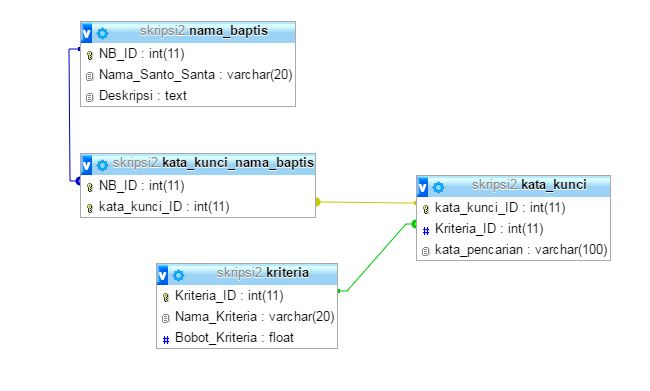
\includegraphics[scale=0.8]{Gambar/desainerdatabase.JPG}
			%\caption{Desain Database}
	%	\label{fig:db4}
	%\end{figure}
	

%\subsection{Bagian Tabel nama\_baptis}
%\label{sec:bagiantabelnb}

%Tabel ini digunakan untuk melihat nama baptis, beserta penjelasan detail dari nama baptis tersebut. %makna atau arti, tanggal pesta, nama lain, dan juga lambang dari nama baptis tersebut . 
	%Pada tabel nama\_baptis terdapat 3 kolom, yaitu:
	
	%\begin{itemize}
		%\item NB\_ID % (Gambar \ref{fig:db1})		
		
	%	\begin{itemize}
	%		\item Digunakan untuk memudahkan pengindeksan.
	%		\item Menggunakan jenis variabel int dengan panjang atau nilai 11.
	%		\item Menggunakan primary key (PK)\\
	%		NB\_ID menggunakan PK, karena PK merupakan kunci utama pada tabel database yang berfungsi sebagai kunci pengurutan data. Pada tabel hanya diperbolehkan memiliki satu PK.
		%	\item Menggunakan \textit{auto increment}\\
		%	NB\_ID menggunakan \textit{auto increment}, karena \textit{auto increment} merupakan tipe \textit{field} integer yang secara otomatis akan bertambah nilainya jika terjadi penambahan \textit{row} pada tabel di mana \textit{field} tersebut berada. Otomatis di sini artinya adalah pada saat memasukkan data baik melalui \textit{statement} INSERT maupun melalui mekanisme data akses lainnya, \textit{field} tersebut tidak perlu dimasukkan nilainya atau cukup diberi nilai NULL, maka MySQL akan menentukan sendiri nilai yang akan diberikan sebagai penambahan baris data tersebut. 
		%\end{itemize}
		
		%\item Nama\_Santo\_Santa %(Gambar \ref{fig:db3})
			
		%\begin{itemize}
		%	\item Digunakan untuk melihat nama santo-santa atau orang-orang kudus.
			%\item Menggunakan jenis variabel varchar dengan panjang atau nilai 20.
		%\end{itemize}
		
		%\item Deskripsi %(Gambar \ref{fig:db2})

%		\begin{itemize}
%			\item Digunakan untuk melihat penjelasan dari masing-masing santo-santa. Penjelasannya terdiri dari makna atau arti, nama lain santo-santa, lambang, dan tanggal pesta. 
	%		\item Menggunakan jenis variabel text.
		%\end{itemize}
%	\end{itemize}


%\subsection{Bagian Tabel kriteria}
%\label{sec:bagiantabelkriteria}

	%Tabel ini digunakan untuk melihat berbagai macam kriteria yang dipilih dan bobot kriteria. Pada tabel kriteria terdapat 3 kolom, yaitu:
	
%\begin{itemize}
%	\item Kriteria\_ID %(Gambar \ref{fig:db7})

	
%	\begin{itemize}
%		\item Digunakan untuk memudahkan pengindeksan.
%		\item Menggunakan jenis variabel int dengan panjang atau nilai 11.
%		\item Menggunakan primary key (PK)
		
	%		Kriteria\_ID menggunakan PK, karena PK merupakan kunci utama pada tabel database yang berfungsi sebagai kunci pengurutan data. Pada tabel hanya diperbolehkan memiliki satu PK.
		%\item Menggunakan \textit{auto increment}
		
		%Kriteria\_ID menggunakan \textit{auto increment}, karena \textit{auto increment} merupakan tipe \textit{field} integer yang secara otomatis akan bertambah nilainya jika terjadi penambahan \textit{row} pada tabel di mana \textit{field} tersebut berada. Otomatis di sini artinya adalah pada saat memasukkan data baik melalui \textit{statement} INSERT maupun melalui mekanisme data akses lainnya, \textit{field} tersebut tidak perlu dimasukkan nilainya atau cukup diberi nilai NULL, maka MySQL akan menentukan sendiri nilai yang akan diberikan sebagai penambahan baris data tersebut.
	%\end{itemize}
	
	%\item Nama\_Kriteria %(Gambar \ref{fig:db8})
	
	%\begin{itemize}
		%\item Digunakan untuk melihat kriteria, seperti arti Santo-Santa, deskripsi, tanggal lahir calon baptis, tanggal pembaptisan, profesi, lambang, serta pesta santo-santa.
		%\item Menggunakan jenis variabel varchar dengan panjang atau nilai 20.

%	\end{itemize}
%	\item Bobot\_Kriteria %(Gambar \ref{fig:db9})
	
	%\begin{itemize}
		%\item Digunakan untuk melihat bobot (W) yang sudah ditentukan untuk masing-masing kriteria.
		%\item Menggunakan jenis variabel float, karena mengandung pecahan.
	%	\end{itemize}
%\end{itemize}

%\subsection{Bagian Tabel Kata\_Kunci}
%\label{sec:bagiantabelkk}
%Tabel ini digunakan untuk melakukan pengelompokkan kata dan dapat yang dicari oleh \textit{user} . Pada tabel kata\_kunci terdapat 3 kolom, yaitu:

	
%	\begin{itemize}
	%	\item Kata\_kunci\_ID %(Gambar \ref{fig:db11})
		
		%	\begin{itemize}
		%\item Digunakan untuk memudahkan pengindeksan.
		%\item Menggunakan jenis variabel int dengan panjang atau nilai 11.
		%\item Menggunakan primary key (PK)
		
			%Kriteria\_ID menggunakan PK, karena PK merupakan kunci utama pada tabel database yang berfungsi sebagai kunci pengurutan data. Pada tabel hanya diperbolehkan memiliki satu PK.
		%\item Menggunakan \textit{auto increment}
		
		%Kriteria\_ID menggunakan \textit{auto increment}, karena \textit{auto increment} merupakan tipe \textit{field} integer yang secara otomatis akan bertambah nilainya jika terjadi penambahan \textit{row} pada tabel di mana \textit{field} tersebut berada. Otomatis di sini artinya adalah pada saat memasukkan data baik melalui \textit{statement} INSERT maupun melalui mekanisme data akses lainnya, \textit{field} tersebut tidak perlu dimasukkan nilainya atau cukup diberi nilai NULL, maka MySQL akan menentukan sendiri nilai yang akan diberikan sebagai penambahan baris data tersebut.
	%\end{itemize}
		
		%\item Kriteria\_ID %(Gambar \ref{fig:db12})
		
		%\begin{itemize}
		%	\item Digunakan untuk mengambil data dari tabel kriteria.
		%	\item Merupakan foreign key (fk) dari tabel kriteria.
		%	\item Menggunakan jenis variabel int dengan panjang atau nilai 11.
		%\end{itemize}
		
		%\item Kata\_pencarian %(Gambar \ref{fig:db13})
		
%		\begin{itemize}
%			\item Digunakan untuk mencari kata yang dimasukkan oleh \textit{user}.
%			\item Menggunakan jenis variabel varchar dengan panjang atau nilai 100.
%			\item Berisi kata yang sudah dikelompokkan agar memudahkan dalam pencarian. Sebagai contoh adalah kata agung dan besar, kata-kata tersebut sudah dijadikan satu kesatuan atau dikelompokkan, agar jika \textit{user} mencari kata ``besar'' yang tidak ada pada suatu deskripsi pada tabel nama\_baptis, akan tetap keluar sebagai hasil \textit{output}. Hasil \textit{output} yang akan keluar untuk kata ``besar'' adalah deskripsi yang mengandung kata ``agung'', karena kata ``besar'' sudah tersimpan dan sudah dikelompokkan dengan kata ``agung'' pada kata\_pencarian.
			
	%	\end{itemize}
	%\end{itemize}
	
	%\subsection{Bagian Tabel Kata\_Kunci\_Nama\_Baptis}
%\label{sec:bagiantabelkknb}
%Tabel ini digunakan untuk membuat tabel kata\_kunci dengan tabel nama\_baptis menjadi satu, sehingga sistem dapat mengetahui yang \textit{user} \textit{input} atau masukkan pada kata\_pencarian dan mencocokan kata yang dimasukkan \textit{user} tersebut dengan nama\_baptis yang ada pada tabel nama\_baptis. Dengan demikian, hasil alternatif akan keluar sesuai dengan yang diinginkan oleh \textit{user}. Pada tabel Kata\_Kunci\_Nama\_Baptis terdapat 2 kolom, yaitu:

%	\begin{itemize}
	%	\item NB\_ID %(Gambar \ref{fig:db16})
		
	
%		\begin{itemize}
%		\item Merupakan foreign key (fk) dari tabel nama\_baptis
%		\item Menggunakan jenis variabel int dengan panjang atau nilai 11.
%		\item Digunakan untuk mengambil data dari tabel nama\_baptis
%		\end{itemize}
		
	%	\item Kata\_Kunci\_ID %(Gambar \ref{fig:db17})
		
%		\begin{itemize}
%		\item Merupakan foreign key (fk) dari tabel kata\_kunci
%		\item Menggunakan jenis variabel int dengan panjang atau nilai 11.
%		\item Digunakan untuk mengambil data dari tabel kata\_kunci
%		\end{itemize}
%\end{itemize}

	%Dari hasil analisis database sebelumnya, dapat disimpulkan bahwa \textit{user} dapat memasukkan \textit{input} berupa kriteria, seperti tanggal lahir calon baptis, tanggal pembaptisan, arti, lambang, profesi dan sebagainya (\textit{input} dapat lebih dari 1). Setelah \textit{user} memasukkan \textit{input} tersebut, maka database akan mencari pada tabel kata\_kunci. Setelah kata yang dicari tersebut sudah ditemukan pada tabel kata\_kunci, kemudian tabel kata\_kunci di JOIN dengan tabel kata\_kunci\_nama\_baptis, untuk mendapatkan NB\_ID dan kriteria. NB\_ID didapatkan untuk mencocokkan kata yang dicari oleh \textit{user} dengan nama baptis yang ada pada database (tabel nama\_baptis), sedangkan kriteria didapatkan agar database dapat mengetahui \textit{user} memasukkan \textit{input} berdasarkan kriteria jenis apa. Setelah mendapatkan kriteria dan NB\_ID, kemudian kedua tabel yang sudah di JOIN harus di JOIN dengan tabel nama\_baptis, agar mendapatkan nama baptis dan deskripsi yang diinginkan oleh \textit{user}.
	
	%\textit{Syntax} JOIN dalam MySQL digunakan untuk menggabungkan beberapa tabel, untuk mendapatkan data \cite{sqljoin}. Menggunakan \textit{Syntax} JOIN karena beberapa tabel dapat digabungkan, sehingga dapat dihasilkan sekumpulan \textit{output} tunggal, dan JOIN menghubungkan record-record yang benar di setiap tabel.
	
	%Hasil pada database merupakan data mentah, dengan kata lain masih belum dapat dikatakan hasil akhir. Data mentah tersebut harus diolah kembali agar mendapatkan hasil yang benar-benar dicari oleh \textit{user}, yaitu dengan menggunakan perhitungan pada metode SAW, dimana membutuhkan bobot pada setiap kriterianya.
	
	
	%akan dilakukan pencarian dengan cara mencocokkan kata yang dicari oleh \textit{user}, yang sudah ada pada tabel kata\_kunci. Setelah menemukan kata yang dicari tersebut pada tabel kata\_kunci, maka tabel tersebut akan di JOIN dengan tabel kata\_kunci\_nama\_baptis. Tabel kata\_kunci\_nama\_baptis akan mencocokkan kata yang dicari oleh \textit{user} dengan tabel nama\_baptis, apakah  Selain menemukan kata yang dicari pada tabel kata\_kunci, sistem juga akan mendapatkan, berdasarkan kriteria apa, user mencari kata tersebut. Kemudian setelah kata yang dicari ditemukan, maka akan di JOIN lagi dengan tabel kriteria untuk mendapatkan bobotnya. Dengan demikian, akan dikeluarkan hasil berupa nama baptis yang sesuai dengan yang diinginkan atau yang dicari oleh \textit{user}.
	
%\subsection{Contoh Kasus SPK Pemilihan Nama Baptis (\textit{user} hanya memasukkan atau memilih 1 kriteria)}
%\label{sec:contohkasus}
	
	%Pada pemilihan nama baptis, \textit{user} akan memasukkan 1 kriteria. Salah satu contoh kriteria adalah arti nama santo-santa. Berikut adalah contoh kode untuk melakukan pencarian daftar nama baptis yang mengandung arti kata ``mulia''.
	
	
	%\begin{lstlisting}
		%select nama_baptis.Nama_Santo_Santa, nama_baptis.deskripsi FROM `nama_baptis` 
		%INNER JOIN kata_kunci_nama_baptis ON nama_baptis.NB_ID=kata_kunci_nama_baptis.NB_ID
		%INNER JOIN kata_kunci ON kata_kunci_nama_baptis.kata_kunci_ID=kata_kunci_ID 
		%INNER JOIN kriteria ON kata_kunci.kriteria_ID=kriteria.kriteria_ID
		%WHERE kata_kunci.kata_pencarian like ``\%mulia\%'' AND kriteria.kriteria_ID = 1
	%\end{lstlisting}
	
	%\begin{figure}[htbp]
	%	\centering
	%		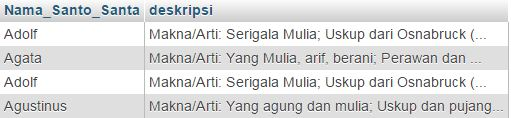
\includegraphics[scale=0.7]{Gambar/contohkasus2.JPG}
	%		\caption{\textit{Hasil Output}}
	%	\label{fig:contohkasus2}
	%\end{figure}
	
  %Hasil \textit{output} yang akan dikeluarkan adalah nama baptis dan deskripsi yang masih mentah (Gambar \ref{fig:contohkasus2}). Pada gambar tersebut, terdapat 4 hasil nama, yang di dalamnya mencakup kata ``mulia''. Keempat nama tersebut belum dapat dikatakan sebagai alternatif, karena pada metode SAW, perlu adanya pembobotan pada masing-masing kriteria, yang menjadikan nama tersebut dapat dikatakan sebagai alternatif. Berikut adalah contoh kode untuk melakukan pencarian daftar nama baptis yang mengandung arti kata ``mulia'' beserta bobotnya pada masing-masing kriteria.

%	, maka akan muncul seperti pada gambar \ref{fig:contohkasus4}, yang mana terdapat bobot pada masing-masing kata yang dicari oleh \textit{user}, berdasarkan kriteria 1, yaitu arti santo-santa, dengan bobot 0.4.
		
%	\begin{lstlisting}
%		select nama_baptis.Nama_Santo_Santa, nama_baptis.deskripsi kriteria.bobot_kriteria FROM `nama_baptis` 
%		INNER JOIN kata_kunci_nama_baptis ON nama_baptis.NB_ID=kata_kunci_nama_baptis.NB_ID
%		INNER JOIN kata_kunci ON kata_kunci_nama_baptis.kata_kunci_ID=kata_kunci_ID 
%		INNER JOIN kriteria ON kata_kunci.kriteria_ID=kriteria.kriteria_ID
%		WHERE kata_kunci.kata_pencarian like ``\%mulia\%'' AND kriteria.kriteria_ID = 1
%	\end{lstlisting}
	

%	\begin{figure}[htbp]
%		\centering
%			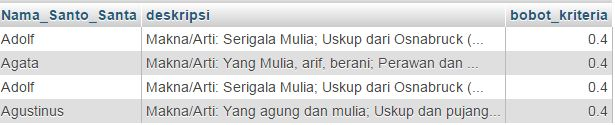
\includegraphics[scale=0.7]{Gambar/contohkasus4.JPG}
%			\caption{\textit{Hasil Output}}
%		\label{fig:contohkasus4}
%	\end{figure}
	
	% Hasil \textit{output} yang akan dikeluarkan adalah nama baptis, deskripsi yang masih mentah dan bobot dari masing-masing kriteria (Gambar\ref{fig:contohkasus4}). Pada gambar tersebut, terdapat 4 hasil nama, yang di dalamnya mencakup kata ``mulia''. Selain terdapat kata ``mulia'', juga terdapat bobot pada tabel tersebut. Keempat nama tersebut belum dapat dikatakan sebagai alternatif, karena pada metode SAW, perlu adanya pembobotan pada masing-masing kriteria, yang menjadikan nama tersebut dapat dikatakan sebagai alternatif.
	
	
	%\subsection{Contoh Kasus SPK Pemilihan Nama Baptis (\textit{user} memasukkan atau memilih lebih dari 1 kriteria)}
%\label{sec:contohkasus1}
	
	%Pada pemilihan nama baptis, \textit{user} akan memasukkan beberapa kriteria. Salah satu contoh kriteria adalah arti nama santo-santa, lambang dan tanggal lahir. Berikut adalah contoh kode untuk melakukan pencarian daftar nama baptis yang mengandung arti kata ``mulia'', lambang ``puteri'' dan tanggal lahir ``juni''.
	
	
	%\begin{lstlisting}
		%select nama_baptis.Nama_Santo_Santa, nama_baptis.deskripsi kriteria.bobot_kriteria FROM `nama_baptis` 
		%INNER JOIN kata_kunci_nama_baptis ON nama_baptis.NB_ID=kata_kunci_nama_baptis.NB_ID
		%INNER JOIN kata_kunci ON kata_kunci_nama_baptis.kata_kunci_ID=kata_kunci.kata_kunci_ID 
		%INNER JOIN kriteria ON kata_kunci.kriteria_ID=kriteria.kriteria_ID
		%WHERE (kata_kunci.kata_pencarian like ``\%mulia\%'' AND kriteria.kriteria_ID = 1) OR (kata_kunci.kata_pencarian like ``\%juni\%'' AND kriteria.kriteria_ID = 3) OR (kata_kunci.kata_pencarian like ``\%puteri\%'' AND kriteria.kriteria_ID = 6)
	%\end{lstlisting}
	
	
%\begin{figure}[htbp]
%		\centering
%			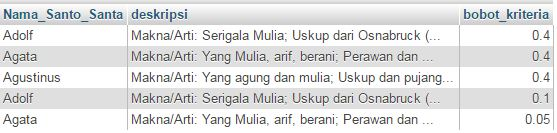
\includegraphics[scale=0.7]{Gambar/contohkasus7.JPG}
%			\caption{\textit{Hasil Output}}
%		\label{fig:contohkasus7}
%	\end{figure}
	
	
	%Hasil \textit{output} yang akan dikeluarkan adalah nama baptis, deskripsi dan bobot dari masing-masing kriteria yang masih mentah (Gambar \ref{fig:contohkasus7}). Yang dimaksud mentah di sini adalah belum dapat dikatakan sebagai alternatif. Pada gambar tersebut, terdapat 5 hasil nama, yang di dalamnya mencakup kata ``mulia''. Yang mencakup kata ``mulia'' terhitung 1 sampai 2 kali muncul. Selain terdapat kata ``mulia'', juga terdapat kata ``puteri'' dan ``juni''. Selain terdapat nama dan deskripsi, juga terdapat bobot pada tabel tersebut. Kelima nama tersebut belum dapat dikatakan sebagai alternatif, karena pada metode SAW, perlu adanya pembobotan pada masing-masing kriteria, yang menjadikan nama tersebut dapat dikatakan sebagai alternatif. Bobot pada masing-masing kriteria berbeda-beda. Bobot pada kriteria arti adalah 0.4, bobot pada kriteria lambang adalah 0.05, dan bobot pada kriteria tanggal lahir adalah 0.1.
	
	
  %Hasil \textit{output} yang akan dikeluarkan sebagai alternatif untuk \textit{user} dapat memilih nama baptis yang cocok adalah dapat dilihat pada gambar \ref{fig:contohkasus7}. Pada gambar tersebut, terdapat 5 hasil nama, yang terhitung terdapat 1 atau 2 kali muncul, yang di dalamnya mencakup kata ``mulia'', ``puteri'', dan ``juni''. Terdapat bobot yang berbeda pada masing-masing nama, yang mana mengacu pada bobot kriteria. Hasil dengan nama Adolf mempunyai 2 data, yang mana di dalamnya mencakup kata ``mulia'', dengan bobot 0.4, dan ``juni'', dengan bobot 0.1. Hasil dengan nama Agata mempunyai 2 data, yang mana di dalamnya mencakup kata ``mulia'', dengan bobot 0.4, dan ``puteri'', dengan bobot 0.05. Dan hasil dengan nama Agustinus hanya mempunyai 1 data, yang mana di dalamnya mencakup kata ``mulia'', dengan bobot 0.4.
	%Keempat nama tersebut belum dapat dikatakan sebagai alternatif, karena pada metode SAW, perlu adanya pembobotan pada masing-masing kriteria, yang menjadikan nama tersebut dapat dikatakan sebagai alternatif. Jika memasukkan \textit{statement} seperti pada gambar \ref{fig:contohkasus3}, maka akan muncul seperti pada gambar \ref{fig:contohkasus4}, yang mana terdapat bobot pada masing-masing kata yang dicari oleh \textit{user}, berdasarkan kriteria 1, yaitu arti santo-santa, dengan bobot 0.4.
	
\section{Analisis \textit{Perangkat Lunak}}
\label{sec:analisisusecase}
\subsection{Diagram \textit{Use Case}}
\label{sec:diagramusecase}
	Diagram \textit{use case} pada perangkat lunak yang akan dibangun hanya mengandung 2 aktor, yaitu calon baptis sebagai \textit{user} dan admin.  Diagram \textit{use case} dapat dilihat pada Gambar  \ref{fig:usecase}.

	\begin{figure}[htbp]
		\centering
			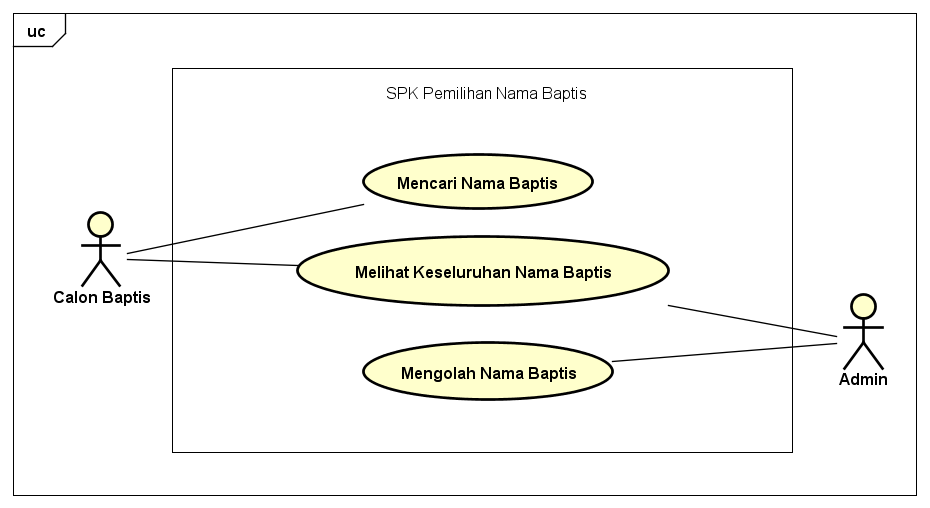
\includegraphics[scale=0.7]{Gambar/usecase.PNG}
			\caption{\textit{Diagram \textit{Use Case} SPK Pemilihan Nama Baptis}}
		\label{fig:usecase}
	\end{figure}

	Berdasarkan hasil analisis  pada subbab analisis kuesioner, dibentuk 3 \textit{use case} dengan 2 aktor, antara lain:
	\begin{itemize}
			\item \textbf{\textit{User}}
				\begin{itemize}
					\item \textbf{Mencari Nama Baptis}

					Calon baptis dapat melihat dan atau memilih kategori apa saja yang dapat digunakan sebagai patokan untuk memilih nama baptis yang cocok, memasukkan \textit{input} seperti kata kunci, dan melihat hasil \textit{output} berupa nama baptis dan deskripsinya. Kategori yang dapat dijadikan patokan atau acuan adalah tanggal lahir calon baptis, tanggal pesta santo-santa, lambang santo-santa, arti nama dari santo-santa, tanggal pembaptisan, deskripsi dari santo-santa, dan profesi dari santo-santa.
					%\item \textbf{Memasukkan \textit{Input}}

					%Calon baptis dapat memasukkan \textit{Input} seperti kata kunci untuk mencari nama baptis yang mereka inginkan.
					%\item \textbf{Melihat Hasil \textit{Output}}

					%Calon baptis dapat melihat hasil \textit{Output} yang dijadikan sebagai alternatif pemilihan nama baptis. Terlebih dahulu calon baptis memasukkan kata kunci dan juga kategori yang diinginkan untuk dijadikan pedoman, agar alternatif dapat dihasilkan dan calon baptis tersebut dapat memilih nama baptis yang diinginkan.
					\item \textbf{Melihat Keseluruhan Nama Baptis}

					Calon baptis atau pengguna umum dapat melihat keseluruhan nama baptis beserta deskripsi di dalamnya.
				\end{itemize}
			\item \textbf{Admin}
				\begin{itemize}
				\item \textbf{Melihat Keseluruhan Nama Baptis}

					Admin dapat melihat keseluruhan nama baptis beserta deskripsi di dalamnya.
					
					\item \textbf{Mengolah Nama Baptis}

					Admin dapat melakukan \textit{update} atau memperbaharui nama baptis, menambahkan nama baptis, dan menghapus nama baptis. Admin dapat memperbaharui nama baptis, serta informasi atau deskripsi yang ada di dalamnya, seperti arti, lambang, profesi dari santo-santa tersebut dan lain sebagainya. Selain dapat memperbaharui, admin juga dapat menambahkan dan menghapus nama baptis serta informasi yang ada di dalamnya.
					%\item \textbf{Menambahkan Nama Baptis}

					%Admin dapat menambahkan nama baptis, dan juga deskripsi atau informasi di dalamnya.
					%\item \textbf{Menghapus Nama Baptis}

					%Admin dapat menghapus nama baptis yang sekiranya tidak terlalu lengkap informasinya.
				\end{itemize}
	\end{itemize}
	
\textbf{Skenario \textit{Use Case}}
\label{sec:skenariousecase}
\begin{enumerate}
\item \textit{User}


                       \begin{enumerate}
                        \item Mencari Nama Baptis
                                \begin{itemize}
                                        \item Nama: Mencari Nama Baptis
                                        \item Aktor: Calon Baptis
                                        \item Deskripsi: Memilih kategori, memasukkan \textit{input}, dan dapat melihat hasil \textit{output} yang sesuai dengan yang dinginkan oleh calon baptis.
                                        \item Kondisi awal: Calon baptis telah membuka web pemilihan nama baptis dan telah memilih kategori, serta memasukkan \textit{input} berupa kata kunci. %msh bingung
                                        \item Kondisi akhir: Web akan menampilkan nama baptis yang dapat dipilih oleh calon baptis.%msh bingung
                                        \item Skenario utama:														
				
				
				\begin{table}[H]
	\centering
	\caption{Tabel Skenario Mencari Nama Baptis}
		\begin{tabular}{| c | p{6cm} |p{6cm} |} \hline
     No  & Aksi & Reaksi Sistem\\ \hline 
		1 & Calon baptis memilih kategori yang telah disediakan, 
		seperti tanggal lahir, profesi, arti dan lain sebagainya. %beserta
		%kata kunci agar memudahkan calon baptis memilih alternatif yang telah di keluarkan. 
		&  Sistem mendapatkan data dari calon baptis berupa kategori yang dipilih.\\ \hline 
		2 & Calon baptis memasukkan \textit{input} berupa kata kunci. & Sistem mendapatkan data dari calon baptis berupa kata kunci dan menampilkan hasil pencarian berdasarkan kata kunci. \\ \hline
		
		3 & Calon baptis melihat dan memilih hasil \textit{output} berupa alternatif nama baptis. & Tidak ada reaksi sistem.\\ \hline
				\end{tabular}
	\label{table:skenario1}
\end{table}
				
				
		                                \end{itemize}
																	 \item Melihat Keseluruhan Nama Baptis

                         \begin{itemize}
                                        \item Nama: Melihat Keseluruhan Nama Baptis
                                        \item Aktor: Calon Baptis atau pengguna umum
                                        \item Deskripsi: Melihat nama baptis dan informasinya
                                        \item Kondisi awal: calon baptis atau pengguna umum telah membuka web pemilihan nama baptis  %msh bingung
                                        \item Kondisi akhir: calon baptis atau pengguna umum dapat melihat nama baptis serta informasinya %msh bingung
                                        \item Skenario utama:														
				
				\begin{table}[H]
	\centering
	\caption{Tabel Skenario Melihat Keseluruhan Nama Baptis (calon baptis/pengguna umum)}
		\begin{tabular}{ | c | p{5cm} |p{5cm} |} \hline
     No  & Aksi & Reaksi Sistem\\ \hline 
				1 & Calon baptis atau pengguna umum memilih menu semua nama baptis.% agar memudahkan calon baptis memilih alternatif yang telah di keluarkan. 
				&  Sistem menampilkan seluruh nama baptis.\\ \hline
		
						\end{tabular}
	\label{table:skenario2}
\end{table}
				
				
				                       
                                \end{itemize}
																\end{enumerate}
																\item Admin
																\begin{enumerate}
																\item Melihat Keseluruhan Nama Baptis
									
                         \begin{itemize}
                                        \item Nama: Melihat keseluruhan nama baptis
                                        \item Aktor: Admin
                                        \item Deskripsi: Melihat nama baptis dan informasinya
                                        \item Kondisi awal: Admin telah membuka web pemilihan nama baptis  %msh bingung
                                        \item Kondisi akhir: Admin dapat melihat nama baptis serta informasinya %msh bingung
                                        \item Skenario utama:														
				
				\begin{table}[H]
	\centering
	\caption{Tabel Skenario Melihat Keseluruhan Nama Baptis (admin)}
		\begin{tabular}{ | c | p{5cm} |p{5cm} |} \hline
     No  & Aksi & Reaksi Sistem\\ \hline 
				1 & Admin memilih menu semua nama baptis.% agar memudahkan calon baptis memilih alternatif yang telah di keluarkan. 
				&  Sistem menampilkan seluruh nama baptis.\\ \hline
		
						\end{tabular}
	\label{table:skenario3}
\end{table}
				
				
																
																       \end{itemize}
																
                                \item Mengolah Nama Baptis
\begin{itemize}
\item Memperbaharui Nama Baptis
\begin{itemize}
                                        \item Nama: Memperbaharui Nama Baptis
                                        \item Aktor: Admin
                                        \item Deskripsi: Dapat memperbaharui data yang sudah ada sebelumnya, menambahkan data baru, dan menghapus data yang tidak terpakai.
                                        \item Kondisi awal: Data lama sudah terdapat pada sistem. %msh bingung
                                        \item Kondisi akhir: Data lama telah diperbaharui dengan data baru. %msh bingung
            
																				
																				\item Skenario utama:														
			\begin{table}[H]
	\centering
	\caption{Tabel Skenario Memperbaharui Nama Baptis}
		\begin{tabular}{ | c | p{5cm} |p{5cm} |} \hline
     No  & Aksi & Reaksi Sistem\\ \hline 
				1 & Admin mengubah nama baptis dan informasinya.% agar memudahkan calon baptis memilih alternatif yang telah di keluarkan. 
				&  Sistem akan mengubah nama baptis dan informasi lama menjadi sesuai dengan \textit{input} admin.\\ \hline
		
						\end{tabular}
	\label{table:skenario4}
\end{table}
			
			

                                \end{itemize}
		\item Menambahkan Nama Baptis

                                \begin{itemize}
                                        \item Nama: Menambahkan nama baptis
                                        \item Aktor: Admin
                                        \item Deskripsi: Dapat menambahkan data baru
                                        \item Kondisi awal: data belum ada pada sistem %msh bingung
                                        \item Kondisi akhir: data baru sudah ditambahkan dan akan ditampilkan%msh bingung
                                        \item Skenario utama:														
				
				
				\begin{table}[H]
	\centering
	\caption{Tabel Skenario Menambahkan Nama Baptis}
		\begin{tabular}{ | c | p{5cm} |p{5cm} |} \hline
     No  & Aksi & Reaksi Sistem\\ \hline 
				1 & Admin menambahkan nama baptis beserta informasinya.% agar memudahkan calon baptis memilih alternatif yang telah di keluarkan. 
				&  Sistem akan menambahkan nama baptis beserta informasinya.\\ \hline
		
						\end{tabular}
	\label{table:skenario5}
\end{table}
				
				

                                \end{itemize}
																\item Menghapus Nama Baptis

                                \begin{itemize}
                                        \item Nama: Menghapus nama baptis
                                        \item Aktor: Admin
                                        \item Deskripsi: Dapat menghapus data yang terlihat tidak begitu lengkap atau tidak begitu terpakai.
                                        \item Kondisi awal: sebelumnya terdapat data pada sistem %msh bingung
                                        \item Kondisi akhir: data telah dihapus dan tidak akan muncul di tampilan%msh bingung
                                        \item Skenario utama:														
				
				\begin{table}[H]
	\centering
	\caption{Tabel Skenario Menghapus Nama Baptis}
		\begin{tabular}{ | c | p{5cm} |p{5cm} |} \hline
     No  & Aksi & Reaksi Sistem\\ \hline 
				1 & Admin menghapus nama baptis dan informasinya.% agar memudahkan calon baptis memilih alternatif yang telah di keluarkan. 
				&  Sistem akan menghapus nama baptis dan informasinya yang telah dipilih oleh admin.\\ \hline
		
						\end{tabular}
	\label{table:skenario6}
\end{table}
				
		
\end{itemize}
\end{itemize}
 \end{enumerate}
 \end{enumerate}%Berdasarkan hasil analisis pada subbab \ref{sec:analisiskuesioner}, 
%\subsection{Bagian Menambahkan Rute}
%\label{sec:menambahkanrute}
%Bagian ini terletak di baris 97-117 dari ``handle.php'' (kode \ref{lst:handle.php}). Bagian ini akan dieksekusi jika terdapat parameter ``\texttt{mode=addtrack}'' pada permintaan POST. Bagian ini berfungsi untuk menambahkan sebuah rute jalan yang dapat ditempuh oleh kendaraan umum tertentu (contoh: angkot).

%Bagian ini diawali dengan memeriksa apakah pengguna memiliki hak akses untuk menambahkan rute atau tidak (baris 98). Lalu memeriksa apakah pengguna mengirimkan data \textit{trackid}, \textit{trackname}, \textit{tracktype}, \textit{penalty}, dan \textit{internalinfo} pada permintaan atau tidak (baris 99-103). Setelah itu, program akan mengecek apakah rute jalan yang ingin ditambahkan pengguna sudah ada atau belum di \textit{database} (106-114). Bila rute jalan belum ada, maka rute jalan akan ditambahkan ke dalam \textit{database} (baris 109) dan \textit{server} akan mengirimkan pesan dalam format JSON (baris 116) sebagai penanda bahwa pengguna berhasil menambahkan rute jalan.

%\subsection{Bagian Mengubah Rute}
%\label{sec:mengubahrute}
%Bagian ini terletak di baris 117-146 dari ``handle.php'' (kode \ref{lst:handle.php}). Bagian ini akan dieksekusi jika terdapat parameter ``\texttt{mode=updatetrack}'' pada permintaan POST. Bagian ini berfungsi untuk mengubah data sebuah rute jalan yang dapat ditempuh oleh kendaraan umum tertentu (contoh: angkot).

%Bagian ini diawali dengan memeriksa apakah pengguna memiliki hak akses untuk mengubah rute atau tidak (baris 118). Lalu memeriksa apakah pengguna mengirimkan data \textit{trackid}, \textit{newtrackid}, \textit{trackname}, \textit{tracktype}, \textit{penalty}, \textit{pathloop}, \textit{transfernodes}  dan \textit{internalinfo} pada permintaan atau tidak (baris 119-126). Setelah itu, \textit{server} akan mengecek apakah rute yang ingin diubah pengguna sudah memenuhi aturan (\textit{trackid} harus sama dengan \textit{newtrackid}) atau tidak (129-143). Bila rute yang ingin diubah maka \textit{server} akan mengirimkan pesan dalam format JSON sebagai penanda bahwa pengguna berhasil mengubah rute rute jalan.

%\subsection{Bagian Melihat Daftar Rute}
%\label{sec:melihatdaftarrute}
%Bagian ini terletak di baris 146-172 dari ``handle.php'' (kode \ref{lst:handle.php}). Bagian ini akan dieksekusi jika terdapat parameter ``\texttt{mode=listtracks}'' pada permintaan POST. Bagian ini berfungsi untuk memberikan daftar rute jalan yang terdapat dalam \textit{database} sistem KIRI.

%Bagian ini diawali dengan memeriksa apakah pengguna memiliki hak akses terhadap rute jalan atau tidak (baris 147). Setelah itu program akan mengambil data daftar rute jalan yang terdapat pada \textit{database} sistem KIRI (baris 149-154). Lalu program juga akan mengambil data daftar tipe rute jalan dari \textit{database} (baris 156-161). Data-data yang diperoleh program (rute jalan dan tipe rute jalan) akan diubah formatnya menjadi sebuah data JSON (baris 164-168). Terakhir, program akan mengirimkan data dalam format JSON tersebut ke pengguna (baris 171).

%\subsection{Bagian Melihat Informasi Rute secara Detail}
%\label{sec:melihatdaftarrutedetail}
%Bagian ini terletak di baris 172-200 dari ``handle.php'' (kode \ref{lst:handle.php}). Bagian ini akan dieksekusi jika terdapat parameter ``\texttt{mode=getdetailstrack}'' pada permintaan POST. Bagian ini berfungsi untuk memberikan informasi detail tentang suatu rute jalan.

%Bagian ini diawali dengan memeriksa apakah pengguna memiliki hak akses terhadap rute jalan atau tidak (baris 173). Lalu program akan memeriksa apakah pengguna memberikan \textit{trackid} pada permintaan atau tidak (baris 174). Selanjutnya program akan mengambil data dari \textit{database} sistem KIRI (baris 177-184). Data yang diperoleh dari \textit{database} tersebut akan diubah formatnya ke dalam format JSON (baris 186-196). Terakhir, program akan mengirimkan data dalam format JSON tersebut ke pengguna (baris 199).

%\subsection{Bagian Menghapus Data Geografis suatu Rute}
%\label{sec:hapusdatageografis}
%Bagian ini terletak di baris 200-209 dari ``handle.php'' (kode \ref{lst:handle.php}). Bagian ini akan dieksekusi jika terdapat parameter ``\texttt{mode=cleargeodata}'' pada permintaan POST. Bagian ini berfungsi untuk menghapus data geografis suatu rute jalan yang terdapat dalam \textit{database} sistem KIRI.

%Bagian ini diawali dengan memeriksa apakah pengguna memiliki hak akses terhadap rute jalan atau tidak (baris 201). Lalu program akan memeriksa apakah pengguna memberikan \textit{trackid} pada permintaan atau tidak (baris 202). Program akan langsung menghapus data geografis rute jalan sesuai dengan \textit{trackid} permintaan pengguna jika \textit{trackid} tersebut terdapat dalam \textit{database} sistem KIRI (baris 204-205). Terakhir, program akan mengirimkan pesan keberhasilan dalam format JSON kepada pengguna (baris 208).

%\subsection{Bagian Impor Data KML}
%\label{sec:imporkml}
%Bagian ini terletak di baris 209-246 dari ``handle.php'' (kode \ref{lst:handle.php}). Bagian ini akan dieksekusi jika terdapat parameter ``\texttt{mode=importkml}'' pada permintaan POST. Bagian ini berfungsi untuk menambahkan data geografis suatu rute dimana data yang ditambahkan berasal dari sebuah \textit{file} dengan format KML (\textit{Keyhole Markup Language}). KML adalah format \textit{file} yang digunakan untuk menampilkan data geografis dalam aplikasi pemetaan\cite{kml}. 

%Bagian ini diawali dengan memeriksa apakah pengguna memiliki hak akses terhadap rute jalan atau tidak (baris 210). Lalu program akan memeriksa apakah pengguna memberikan \textit{trackid} pada permintaan atau tidak (baris 211). Selanjutnya program akan memeriksa apakah \textit{file} pengguna memberikan \textit{file} dengan format sesuai atau tidak (baris 213-218). Pada baris 219-228 program akan mengambil data LineString yang terdapat pada \textit{file} dengan menggunakan teknik \textit{regular expression} (baris 224, referensi subbab \ref{sec:regex}). Baris 231-239 program akan membangun data LineString yang semula dalam format KML menjadi format WKT (subbab \ref{sec:wktformat}). Program akan menambahkan data LineString dalam WKT tersebut ke dalam \textit{database} sesuai dengan \textit{trackid} yang diberikan pengguna (baris 241-243). Terakhir, program akan mengirimkan pesan dalam format JSON sebagai penanda bahwa pengguna berhasil melakukan import data KML (baris 245).

%\subsection{Bagian Menghapus Rute}
%\label{sec:hapusrute}
%Bagian ini terletak di baris 246-261 dari ``handle.php'' (kode \ref{lst:handle.php}). Bagian ini akan dieksekusi jika terdapat parameter ``\texttt{mode=deletetrack}'' pada permintaan POST. Bagian ini berfungsi untuk menghapus suatu rute jalan yang terdapat dalam sistem KIRI.

%Bagian ini diawali dengan memeriksa apakah pengguna memiliki hak akses terhadap rute jalan atau tidak (baris 247). Lalu program akan memeriksa apakah pengguna memberikan \textit{trackid} pada permintaan atau tidak (baris 248). Program akan memeriksa apakah terdapat {trackid} yang sesuai dengan {trackid} yang ada pada \textit{database} KIRI (baris 250-259). Bila terdapat \textit{trackid} yang sesuai, maka program akan menghapus rute jalan tersebut. Terakhir, program akan mengirimkan pesan keberhasilan dalam format JSON kepada pengguna (baris 260).

%\subsection{Bagian Melihat Daftar API \textit{Keys}}
%\label{sec:lihatapikeys}
%Bagian ini terletak di baris 261-279 dari ``handle.php'' (kode \ref{lst:handle.php}). Bagian ini akan dieksekusi jika terdapat parameter ``\texttt{mode=listapikeys}'' pada permintaan POST. Bagian ini berfungsi untuk memberikan daftar API \textit{keys} yang terdapat dalam database sistem KIRI.

%Bagian ini diawali dengan memeriksa apakah pengguna memiliki hak akses terhadap penggunaan API atau tidak (baris 262). Setelah itu program akan mengambil data daftar API \textit{keys} yang terdapat pada \textit{database} sistem KIRI (baris 264-269). Data-data yang diperoleh program akan diubah formatnya menjadi sebuah data JSON (baris 272-275). Terakhir, program akan mengirimkan data dalam format JSON tersebut ke pengguna (baris 278).

%\subsection{Bagian Menambahkan API \textit{Key}}
%\label{sec:tambahapikey}
%Bagian ini terletak di baris 279-299 dari ``handle.php'' (kode \ref{lst:handle.php}). Bagian ini akan dieksekusi jika terdapat parameter ``\texttt{mode=addapikey}'' pada permintaan POST. Bagian ini berfungsi untuk menambahkan sebuah data API \textit{key} ke dalam sistem KIRI.

%Bagian ini diawali dengan memeriksa apakah pengguna memiliki hak akses terhadap API \textit{keys} atau tidak (baris 280). Lalu memeriksa apakah pengguna mengirimkan data \textit{domainfilter} dan \textit{description} pada permintaan atau tidak (baris 281-282). Setelah itu, program akan membangun sebuah API key secara acak (baris 283). Program akan menambahkan data API \textit{key} sesuai dengan data yang dikirimkan pengguna ke dalam \textit{database} KIRI (baris 286) dan mencatat proses penambahan tersebut ke dalam \textit{database} (baris 289). Terakhir, program akan membangun sebuah pesan keberhasilan dalam format JSON (baris 292-295) dan mengirimkan pesan tersebut kepada pengguna (baris 298).

%\subsection{Bagian Mengubah API \textit{Key}}
%\label{sec:ubahapikey}
%Bagian ini terletak di baris 299-317 dari ``handle.php'' (kode \ref{lst:handle.php}). Bagian ini akan dieksekusi jika terdapat parameter ``\texttt{mode=updateapikey}'' pada permintaan POST. Bagian ini berfungsi untuk mengubah data sebuah API \textit{key} pada \textit{database} sistem KIRI.

%Bagian ini diawali dengan memeriksa apakah pengguna memiliki hak akses terhadap API \textit{keys} atau tidak (baris 300). Lalu memeriksa apakah pengguna mengirimkan data \textit{apikey}, \textit{domainfilter}, dan \textit{description} pada permintaan atau tidak (baris 301-303). Setelah itu, program akan memeriksa apakah pengguna yang bersangkutan adalah pemilik API \textit{key} yang ingin diubah atau bukan (baris 305-311). Lalu program mengubah data API \textit{key} yang terdapat dalam database (baris 312) sesuai dengan permintaan pengguna. Terakhir, program akan mengirimkan pesan dalam format JSON sebagai penanda bahwa pengguna berhasil mengubah rute jalan.

%\subsection{Bagian \textit{Register}}
%\label{sec:bagianregister}
%Bagian ini terletak di baris 317-341 dari ``handle.php'' (kode \ref{lst:handle.php}). Bagian ini akan dieksekusi jika terdapat parameter ``\texttt{mode=register}'' pada permintaan POST. Bagian ini berfungsi untuk melakukan pendaftaran sebagai pengguna KIRI \textit{Dashboard}. Pendaftaran ini berguna agar pengguna bisa mendapatkan hak akses terhadap fitur-fitur yang terdapat dalam KIRI \textit{Dashboard}.

%Bagian ini diawali dengan memeriksa apakah pengguna memberikan \textit{email}, \textit{fullname}, dan \textit{company} pada permintaan atau tidak (baris 318-320). Setelah itu, program akan memeriksa \textit{database} apakah data pengguna yang ingin dibuat sudah ada atau belum (baris 323-327). Bila belum ada, maka program akan membangun sebuah sandi secara acak untuk pengguna (baris 330-332). Program akan menambahkan data pengguna beserta sandi yang telah dibangun ke dalam \textit{database} sistem KIRI (baris 333). Sandi yang telah dibangun program juga dikirimkan ke alamat \textit{email} pengguna (baris 335). Lalu program mencatat proses tersebut ke dalam statistik \textit{database} sistem KIRI. Terakhir, program akan mengirimkan pesan dalam format JSON sebagai penanda bahwa pengguna berhasil melakukan proses registrasi (baris 340).

%\subsection{Bagian Melihat Data Pribadi Pengguna}
%\label{sec:lihatdatadiri}
%Bagian ini terletak di baris 341-362 dari ``handle.php'' (kode \ref{lst:handle.php}). Bagian ini akan dieksekusi jika terdapat parameter ``\texttt{mode=getprofile}'' pada permintaan POST. Bagian ini berfungsi untuk memberikan informasi mengenai data pribadi pengguna.

%Bagian ini diawali dengan memeriksa apakah data pengguna dengan \textit{email} yang dimiliki pengguna pada saat sesi tersebut ada atau tidak (baris 344-345). Jika data pengguna ditemukan maka program akan mengambil dan membangun data pengguna (baris 346-351). Data pengguna yang dibangun tersebut kemudian diubah ke dalam format JSON (baris 355-359). Terakhir, program mengirimkan data dalam format JSON yang telah dibangun kepada pengguna (baris 361).

%\subsection{Bagian Mengubah Data Pribadi Pengguna}
%\label{sec:ubahdatadiri}
%Bagian ini terletak di baris 362-380 dari ``handle.php'' (kode \ref{lst:handle.php}). Bagian ini akan dieksekusi jika terdapat parameter ``\texttt{mode=updateprofile}'' pada permintaan POST. Bagian ini berfungsi untuk mengubah data pribadi pengguna yang sudah terdaftar dalam sistem KIRI.

%Bagian ini diawali dengan memeriksa apakah pengguna memberikan \textit{password}, \textit{fullname}, dan \textit{company} pada permintaan atau tidak (baris 364-366). Bila pengguna memberikan \textit{password} dengan nilai \texttt{NULL} maka program akan membangun \textit{password} secara acak dan menambahkan \textit{password} tersebut ke dalam \textit{database} sistem KIRI sesuai dengan \textit{email} pengguna pada saat sesi tersebut (kode 369-374). Lalu program akan mengubah semua data pribadi pengguna sesuai dengan data yang diberikan oleh pengguna (baris 375-376). Terakhir, program mengirimkan pesan keberhasilan dalam format JSON kepada pengguna (baris 379).

%\section{Analisis \textit{Database} Sistem Kini}
%\label{sec:analisisdatabasesistemkini}
%Sistem KIRI menggunakan perangkat lunak MySQL sebagai sarana penyimpanan untuk mengolah data. Seperti yang dijelaskan pada subbab sebelumnya (subbab \ref{sec:analisissistemkini}) terdapat sebuah \textit{folder} yang menyimpan \textit{file-file} untuk membangun \textit{database} sistem KIRI, yaitu: \textit{folder} ``sql'' (gambar \ref{fig:3_strukturkiri}). Berdasarkan hasil analisa dan wawancara dengan kontributor kode KIRI, berikut adalah penjelasan mengenai isi \textit{folder} ``sql'' (gambar \ref{fig:4_struktursql}):
%\begin{enumerate}
%	\item \textit{file} ``.gitignore'', merupakan \textit{file} yang menyimpan daftar \textit{file} yang tidak perlu dikirimkan ke tempat penyimpanan GitHub karena \textit{file-file} tersebut dibangkitkan oleh sistem.
%	\item \textit{file} ``tirtayasa\_structure.sql'', merupakan \textit{file} untuk membangun tabel-tabel serta kolom-kolom (pada setiap tabel) \textit{database} sistem KIRI.
%	\item \textit{file} ``tirtayasa.sql'', merupakan \textit{file} untuk membangun isi dari kolom-kolom setiap tabel, yaitu \textit{record-record} awal.
%\end{enumerate}


%\section{Analisis Sistem Usulan}
%\label{sec:analisissistemusulan}
%Berdasarkan hasil analisa dan wawancara dengan kontributor kode pada subbab sebelumnya (subbab \ref{sec:analisissistemkini} dan subbab \ref{sec:analisisdatabasesistemkini}) didapatkan poin-poin bahwa:
%\begin{enumerate}
	%\item KIRI \textit{Dashboard} terdiri dari dua bagian penting, yaitu bagian pertama adalah \textit{file} dan \textit{folder} yang bersifat statis, yaitu: ``index.html'', ``bukitjariangwt/'', dan ``images/'', serta bagian kedua adalah ``handle.php'' yang bertugas menangani permintaan-permintaan (dari ``index.html'') pada sisi \textit{server}.
	%\item KIRI \textit{Dashboard server side} (\textit{file} ``handle.php'') terbagi menjadi 16 bagian dalam menangani permintaan.
	%\item Perangkat lunak pengolahan data yang digunakan oleh sistem KIRI adalah MySQL.
%\end{enumerate}

%Dalam memodelkan KIRI \textit{Dashboard} dengan menggunakan Play Framework perlu memperhatikan beberapa hal, yaitu: MVC, \textit{routes}, dan \textit{database}.

%\subsection{Routes}
%\label{sec:routesusulan}
%Kebutuhan KIRI \textit{Dashboard} adalah pemetaan untuk ke 2 bagian, yaitu:
%\begin{enumerate}
%	\item Pemetaan URL untuk menangani tampilan (\textit{View}) KIRI \textit{Dashboard}. Hanya 1 pemetaan untuk tampilan (walau fitur KIRI \textit{Dashboard} banyak) yang dibutuhkan karena kode KIRI pada sistem kini telah menggunakan permodelan sistem yang menggunakan AJAX dalam mengatur proses permintaan datanya. Penggunaaan AJAX memungkinkan suatu aplikasi berbasis web tidak perlu melakukan permintaan berulang-ulang untuk tampilan yang umumnya sama (meningkatkan kecepatan saat \textit{browsing}).
%	\item Pemetaan URL untuk menangani permintaan dari tampilan, yaitu KIRI \textit{Dashboard server side} ((\textit{Controller})). Bagian pemetaan ini yang nantinya akan menangani 16 bagian permintaan yang dilakukan bagian tampilan KIRI \textit{Dashboard}.
%\end{enumerate}

%\subsection{\textit{Views}}
%\label{sec:viewusulan}
%Seperti yang telah dijelaskan pada subbab sebelumnya bahwa bagian tampilan KIRI \textit{Dashboard} dibuat dengan menggunakan perangkat GWT dimana kode yang dihasilkan sangat sulit untuk dipelajari. Walau sulit dipelajari, bagian tampilan KIRI \textit{Dashboard} memiliki keuntungan sendiri karena bersifat statis (dijelaskan oleh kontributor kode). Sifat statis ini memudahkan permodelan karena dengan begitu kode dapat disalin apa adanya ke sistem usulan. Pada Play Framework \textit{file-file} yang bersifat statis seperti ini dapat disimpan pada bagian \textit{folder} ``public/''. Akibat dari disimpanny \textit{file-file} tampilan ke \textit{folder} ``public/'' adalah bagian \textit{views} pada struktur Play Framework akan kosong. Kosongnya bagian \textit{views} menyebabkan seolah-olah Play Framework tidak menggunakan konsep MVC.

%\subsection{\textit{Controllers}}
%\label{sec:controllerusulan}
%Pada bagian ini akan dibuat sebuah metode yang akan menangani permintaan dari \textit{views} sistem usulan. Bagian ini berfungsi seperti ``handle.php'', yaitu menangani 16 jenis permintaan seperti yang telah dijelaskan pada subbab sebelumnya.

%\subsection{\textit{Models}}
%\label{sec:modelusulan}
%Tidak ada bagian yang perlu diubah menjadi \textit{models}, maka bagian ini tidak perlu ada pada sistem usulan.

%\subsection{\textit{Database}}
%\label{sec:databaseusulan}
%Sistem kini menggunakan MySQL sebagai perangkat pengolah datanya. Aplikasi yang dibuat dengan Play Framework memungkinkan untuk menggunakan MySQL sebagai perangkat pengolahan datanya. Untuk itu bagian \textit{database} sistem kini dapat disalin apa adanya. Perbedaan pada sistem usulan adalah pada penulisan kode dalam melakukan koneksi dan eksekusi suatu \textit{query} ke MySQL karena sebelumnya menggunakan bahasa PHP dan Play Framework menggunakan bahasa Java (JDBC).}{}
\ifdefstring{\vbabd}{1}{\include{Bab/bab4}}{}
\ifdefstring{\vbabe}{1}{\include{Bab/bab5}}{}
\ifdefstring{\vbabf}{1}{\include{Bab/bab6}}{}
\ifdefstring{\vbabg}{1}{\include{Bab/bab7}}{}
\ifdefstring{\vbabh}{1}{\include{Bab/bab8}}{}
\ifdefstring{\vbabi}{1}{\include{Bab/bab9}}{}

\bibliographystyle{ieeetr}
\bibliography{pustaka}

\appendix
\apptoc

\tampillmp{\vlmp}
\ifdefstring{\vlmpa}{1}{\chapter{The Program}
\label{app:A}

The interface of the program is shown in Figure~\ref{fig:appxa2}:

\begin{figure}[H]
\centering
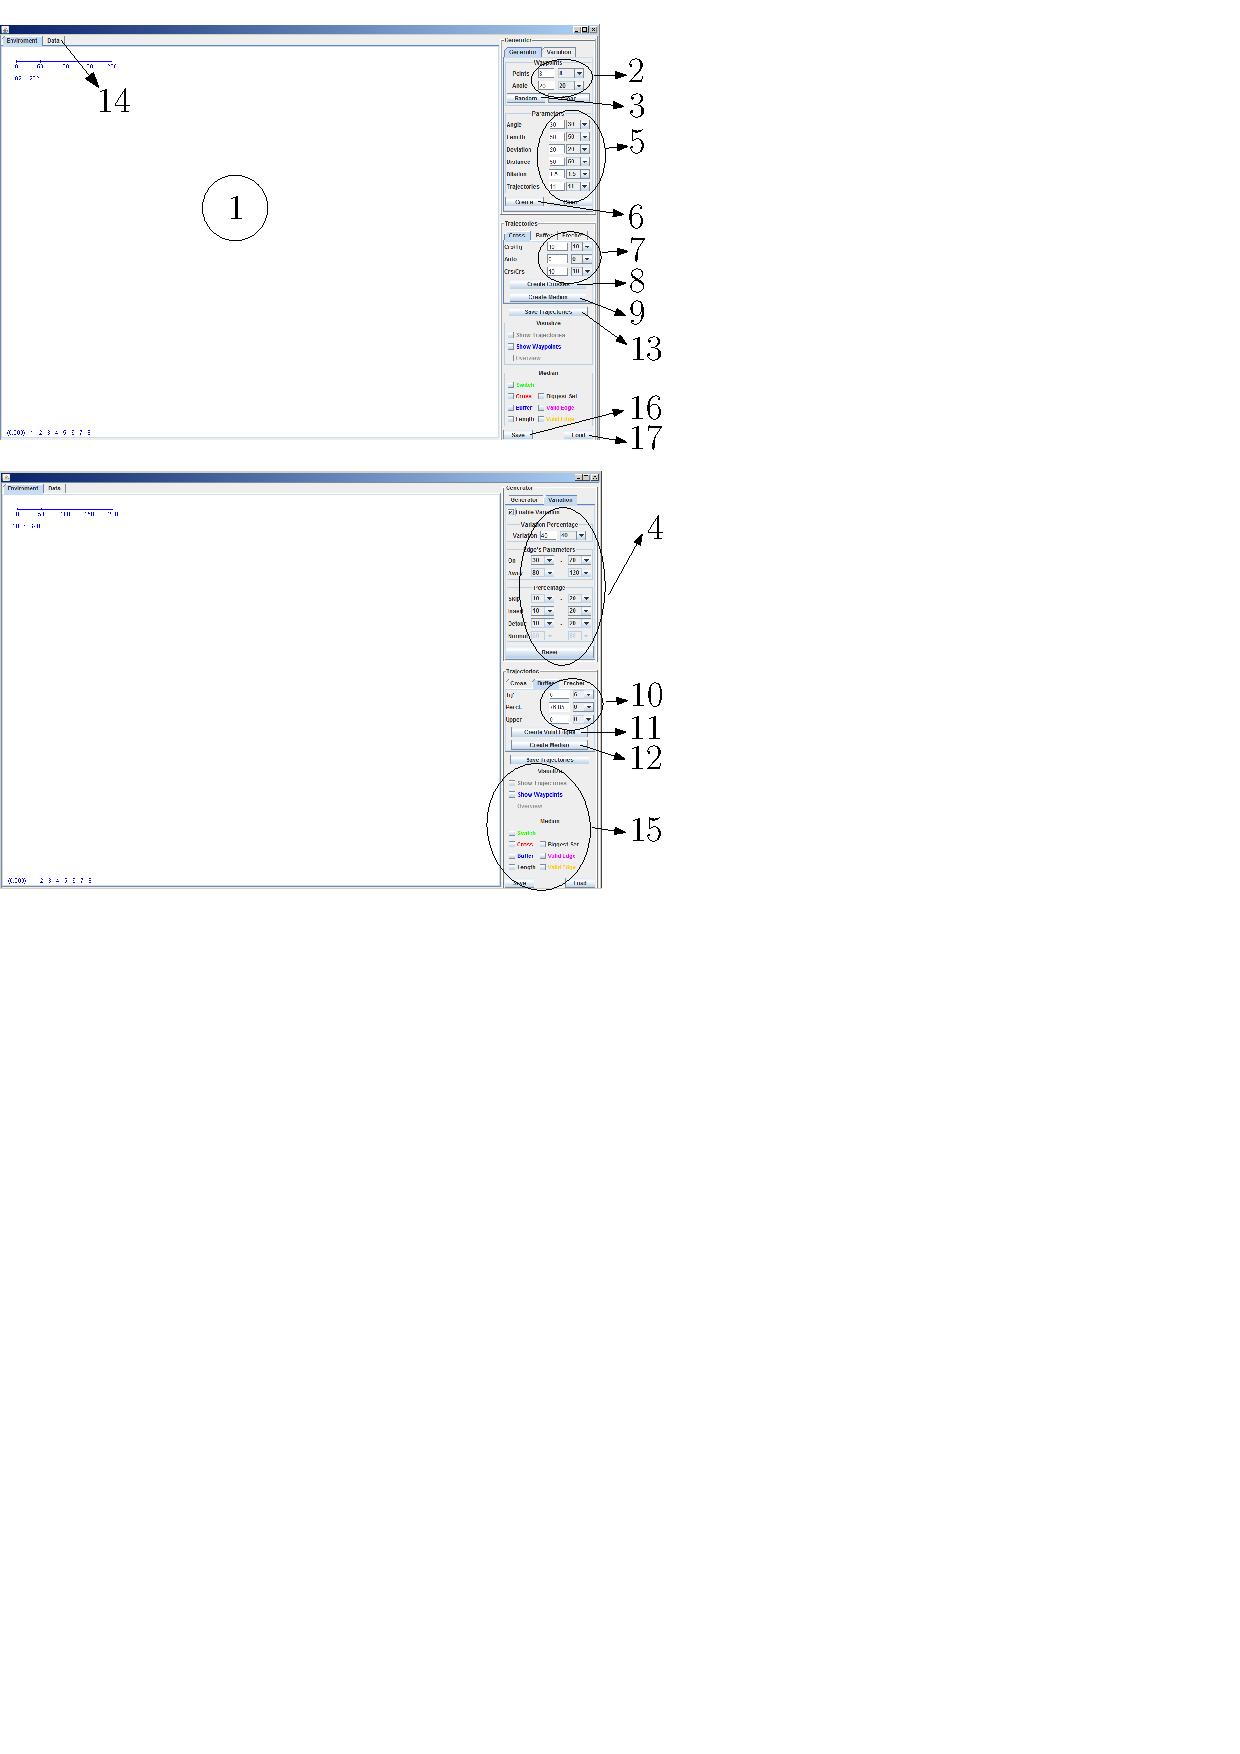
\includegraphics[scale=1]{Gambar/appxa2}
\caption[Interface of the program]{Interface of the program} 
\label{fig:appxa2}
\end{figure}

Step by step to compute the median trajectory using the program:
\begin{enumerate}
\item
Create several waypoints. 
Click anywhere in the ``Environment'' area(1) or create them automatically by setting the parameters for waypoint(2) or clicking the button ``Random''(3).
\item
The ``Variation'' tab could be used to create variations by providing values needed to make them(4).
\item
Create a set of trajectories by setting all parameters(5) and clicking the button ``Create''(6).
\item
Compute the median using the homotopic algorithm: 
\begin{itemize}
\item Define all parameters needed for the homotopic algorithm(7).
\item Create crosses by clicking the ``Create Crosses'' button(8).\item Compute the median by clicking the ``Compute Median'' button(9).
\end{itemize}
\item
Compute the median using the switching method and the buffer algorithm: 
\begin{itemize}
\item Define all parameters needed for the buffer algorithm(10).
\item Create valid edges by clicking the ``Create Valid Edges''button(11). 
\item Compute the median by clicking the ``Compute Median''button(12).
\end{itemize}
\item
Save the resulting median by clicking the ``Save Trajectories'' button(13).
The result is saved in the computer memory and can be seen in ``Data'' tab(14) 
\item 
The set of trajectories and its median trajectories will appear in the ``Environment'' area(1) and the user can change what to display by selecting various choices in ``Visualize'' and ``Median'' area(15).
\item
To save all data to the disk, click the ``Save''(16) button. A file dialog menu will appear.
\item
To load data from the disk, click the ``Load''(17) button.
\end{enumerate}}{}
\ifdefstring{\vlmpb}{1}{\chapter{The Source Code}
\label{app:B}

%selalu gunakan single spacing untuk source code !!!!!
\singlespacing 
% language: bahasa dari kode program
% terdapat beberapa pilihan : Java, C, C++, PHP, Matlab, R, dll
%
% basicstyle : ukuran font untuk kode program
% terdapat beberapa pilihan : tiny, scriptsize, footnotesize, dll
%
% caption : nama yang akan ditampilkan di dokumen akhir, lihat contoh
\begin{lstlisting}[language=Java,basicstyle=\tiny,caption=MyFurSet.java]

import java.util.ArrayList;
import java.util.Collections;
import java.util.HashSet;

/**
 *
 * @author Lionov
 */

//class for set of vertices close to furthest edge
public class MyFurSet {
    protected int id;                                  //id of the set
    protected MyEdge FurthestEdge;                     //the furthest edge
    protected HashSet<MyVertex> set;                   //set of vertices close to furthest edge
    protected ArrayList<ArrayList<Integer>> ordered;   //list of all vertices in the set for each trajectory
    protected ArrayList<Integer> closeID;              //store the ID of all vertices
    protected ArrayList<Double> closeDist;             //store the distance of all vertices
    protected int totaltrj;                            //total trajectories in the set

    /**
     * Constructor
     * @param id : id of the set
     * @param totaltrj : total number of trajectories in the set
     * @param FurthestEdge : the furthest edge
     */
    public MyFurSet(int id,int totaltrj,MyEdge FurthestEdge) {
        this.id = id;
        this.totaltrj = totaltrj;
        this.FurthestEdge = FurthestEdge;
        set = new HashSet<MyVertex>();
        ordered = new ArrayList<ArrayList<Integer>>();
        for (int i=0;i<totaltrj;i++) ordered.add(new ArrayList<Integer>());
        closeID = new ArrayList<Integer>(totaltrj);
        closeDist = new ArrayList<Double>(totaltrj);
        for (int i = 0;i <totaltrj;i++) {
            closeID.add(-1);
            closeDist.add(Double.MAX_VALUE);
        }
    }

    /**
     * set a vertex into the set
     * @param v : vertex to be added to the set
     */
    public void add(MyVertex v) {
        set.add(v);
    }

    /**
     * check whether vertex v is a member of the set
     * @param v : vertex to be checked
     * @return true if v is a member of the set, false otherwise
     */
    public boolean contains(MyVertex v) {
        return this.set.contains(v);
    }
}
\end{lstlisting}}{}
\ifdefstring{\vlmpc}{1}{\include{Lampiran/lampC}}{}
\ifdefstring{\vlmpd}{1}{\include{Lampiran/lampD}}{}
\ifdefstring{\vlmpe}{1}{\include{Lampiran/lampE}}{}
\ifdefstring{\vlmpf}{1}{\include{Lampiran/lampF}}{}
\ifdefstring{\vlmpg}{1}{\include{Lampiran/lampG}}{}
\ifdefstring{\vlmph}{1}{\include{Lampiran/lampH}}{}
\ifdefstring{\vlmpi}{1}{\include{Lampiran/lampI}}{}

\end{document}

%=============================================================================
% Perubahan pada versi 8 (31-05-2015): 
%	- penambahan default data untuk beberapa keterangan dan digunakan sebagai 
%	  template dengan tanda << & >> . Data yang diubah defaultnya adalah: nama skripsi
%	  nama prodi, beserta bahasa inggrisnya.
%   - Keywords dan kata kunci di abstrak ditambahkan noindent + perbaikan lainnya
%   - Perbaikan untuk halaman tidak kosong tanpa nomor halaman romawi
% Perubahan pada versi 7 (27-05-2014)
%	- penambahan perintah \raggedbottom untuk menghilangkan area kosong akibat 
%	  penempatan gambar yang tidak sempurna
% Perubahan pada versi 6 (10-11-2013)
%	- perbaikan pada abstract dengan paragraf lebih dari satu: perbaikan vertical spacing
%	- perbaikan pada tampilan bab dan lampiran: tidak perlu menuliskan apapun untuk 
%	  menampilkan semuanya (di data.tex) atau -1 jika tidak ada lampiran
%	- halaman bernomor genap untuk halaman romawi sudah dimunculkan
%	- Kurikulum 2013 : perubahan nama buku skripsi 
% Perubahan pada versi 5 (21-10-2012)
%	- halaman terakhir setiap bab tidak ada headernya jika kosong
% Perubahan pada versi 4 (06-08-2012)
% 	- penggabungan main.tex, depan.tex dan setup.tex menjadi main.tex
% 	- menambahkan keterangan di lampiran untuk kode program 
% 	- ukuran font dapat diubah langsung di tiap lampiran
% Perubahan pada versi 3 (09-07-2012): 
%	- Tidak ada perubahan di file ini
% Perubahan pada versi 2 (08-07-2012):
% 	- "Daftar Referensi" tidak perlu diubah secara manual (tidak perlu mengubah file bahasai.ldf)
% 	- Bahasa Indonesia dari abstract adalah abstrak (secara otomatis), bukan ringkasan
% 	- Spasi pada buku dokumen final adalah onehalfspacing
% Versi 1 (08-11-2011)
%=============================================================================
%=============================================================================
% depan.tex v2 (09-07-2012)
% Perubahan pada versi 2:
% - Menambahkan halaman depan dalam bahasa inggris
% Versi 1 (08-11-2011)
%=============================================================================
% setup.tex v2 (08-07-2012)
% Perubahan pada versi 2:
% - Menambahkan perintah untuk judulINA dan judulENG
% - Menghapus \usepackage{microtype}, yang pada beberapa kasus menjadi masalah
% Versi 1 (08-11-2011)
%=============================================================================